\chapter{Bundles}
\section{Vector bundles}
\subsection{Vector bundles}
Let $M$ be a topological space. A \textbf{real vector bundle of rank $\bm{k}$ over $\bm{M}$} is a topological space $E$ together with a surjective continuous map $\pi:E\to M$ satisfying the following conditions:
\begin{itemize}
\item For each $p\in M$, the fiber $E_p=\pi^{-1}(p)$ over $p$ is endowed with the structure of a $k$-dimensional real vector space.
\item For each $p\in M$, there exist a neighborhood $U$ of $p$ in $M$ and a homeomorphism $\varPhi:\pi^{-1}(U)\to U\times\R^k$ (called a \textbf{local trivialization} of $E$ over $U$), satisfying the following conditions:
\begin{itemize}
\item $\pi_U\circ\varPhi=\pi$, where $\pi_U:U\times\R^k\to U$ is the projection.
\item for each $q\in U$, the restriction of $\varPhi$ to $E_q$ is a vector space isomorphism from $E_q$ to $\{q\}\times\R^k\cong\R^k$.
\end{itemize}
\end{itemize}
\begin{figure}[htbp]
\centering
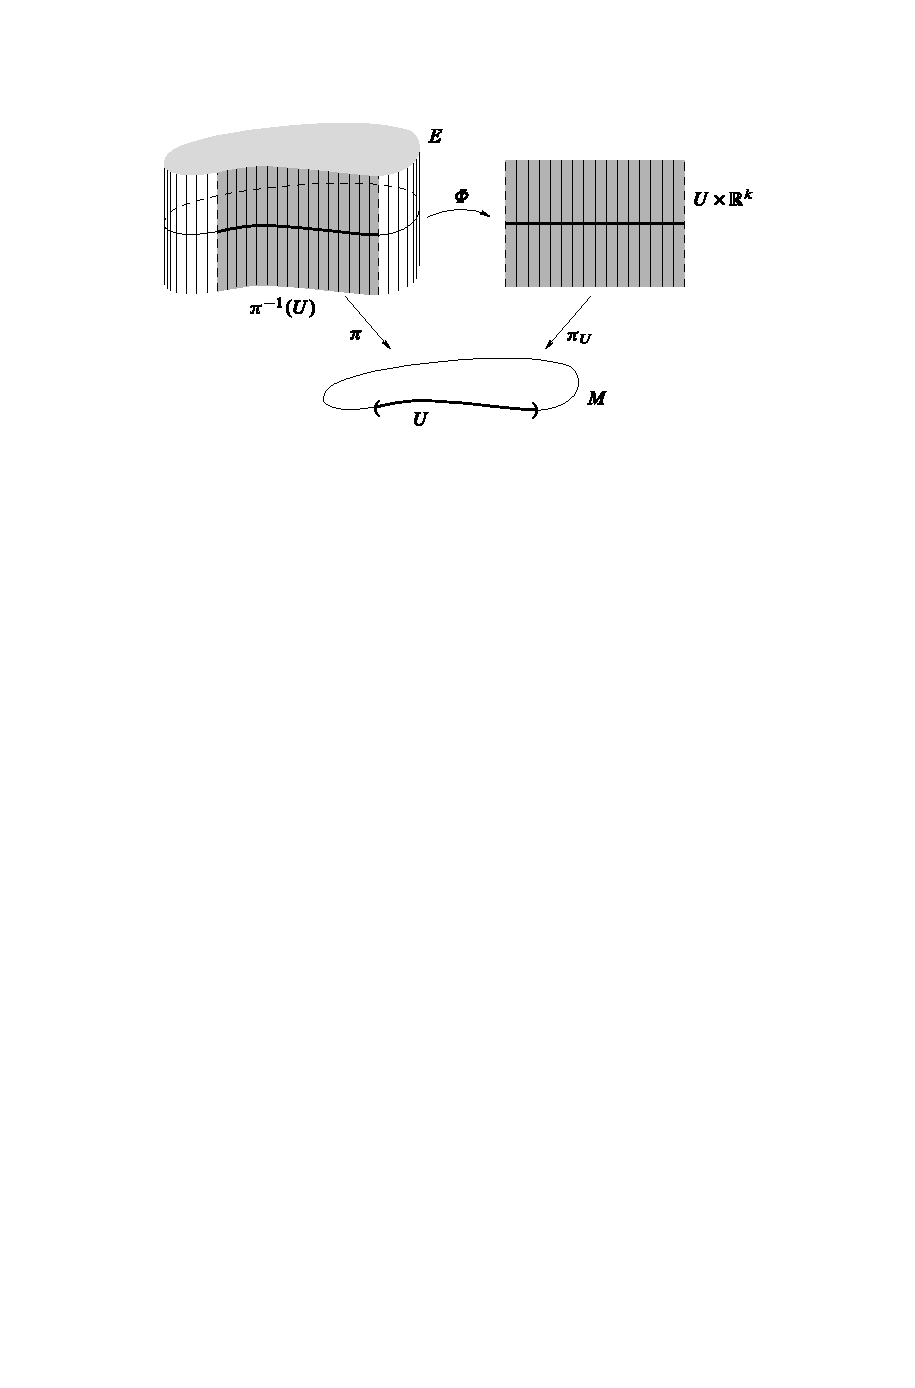
\includegraphics{local-trivialization}
\caption{A local trivialization of a vector bundle.}
\end{figure}\par
If $M$ and $E$ are smooth manifolds with or without boundary, $\pi$ is a smooth map, and the local trivializations can be chosen to be diffeomorphisms, then $E$ is called a \textbf{smooth vector bundle}. In this case, we call any local trivialization that is a diffeomorphism onto its image a \textbf{smooth local trivialization}.\par
A rank-$1$ vector bundle is often called a \textbf{real line bundle}. \textbf{Complex vector bundles} are defined similarly, with real vector space replaced by complex vector space and $\R^k$ replaced by $\C^k$ in the definition. The space $E$ is called the \textbf{total space} of the bundle, $M$ is called its \textbf{base}, and $\pi$ is its projection.
\begin{proposition}
Suppose $E$ is a smooth vector bundle over $M$. Then the projection map $\pi:E\to M$ is a surjective smooth submersion.
\end{proposition}
\begin{proof}
For each point of $E$, there is a local trivialization $\varPhi$ such that $\pi=\pi_U\circ\varPhi$. Since $\pi_U$ and $\varPhi$ are both submersion, it follows that $\pi$ is a submersion.
\end{proof}
If there exists a local trivialization of $E$ over all of $M$ (called a \textbf{global trivialization} of $E$), then $E$ is said to be a \textbf{trivial bundle}. In this case, $E$ itself is homeomorphic to the product space $M\times\R^k$. If $E\to M$ is a smooth bundle that admits a smooth global trivialization, then we say that $E$ is \textbf{smoothly trivial}. In this case $E$ is diffeomorphic to $M\times\R^k$, not just homeomorphic. For brevity, when we say that a smooth bundle is trivial, we always understand this to mean smoothly trivial, not just trivial in the topological sense.
\begin{example}[\textbf{Product Bundles}]
One particularly simple example of a rank $k$ vector bundle over any space $M$ is the product space $E=M\times\R^k$ with $\pi=\pi_1:M\times\R^k\to M$ as its projection. Any such bundle, called a product bundle, is trivial (with the identity map as a global trivialization). If $M$ is a smooth manifold with or without boundary, then $M\times\R^k$ is smoothly trivial.
\end{example}
Although there are many vector bundles that are not trivial, the only one that is easy to visualize is the following.
\begin{example}[\textbf{The Möbius Bundle}]\label{Mobius bundle}
Define an equivalence relation on $\R^2$ by declaring that $(x,y)\sim(x',y')$ if and only if $(x',y')=(x+n,(-1)^ny)$ for some $n\in\Z$. Let $E=\R^2/\sim$ denote the quotient space, and let $q:\R^2\to E$ be the quotient map. For any $r>0$, the image under the quotient map $q$ of the rectangle $[0,1]\times[-r,r]$ is a smooth compact manifold with boundary called a \textbf{M\"obius band}.
\begin{figure}[htbp]
\centering
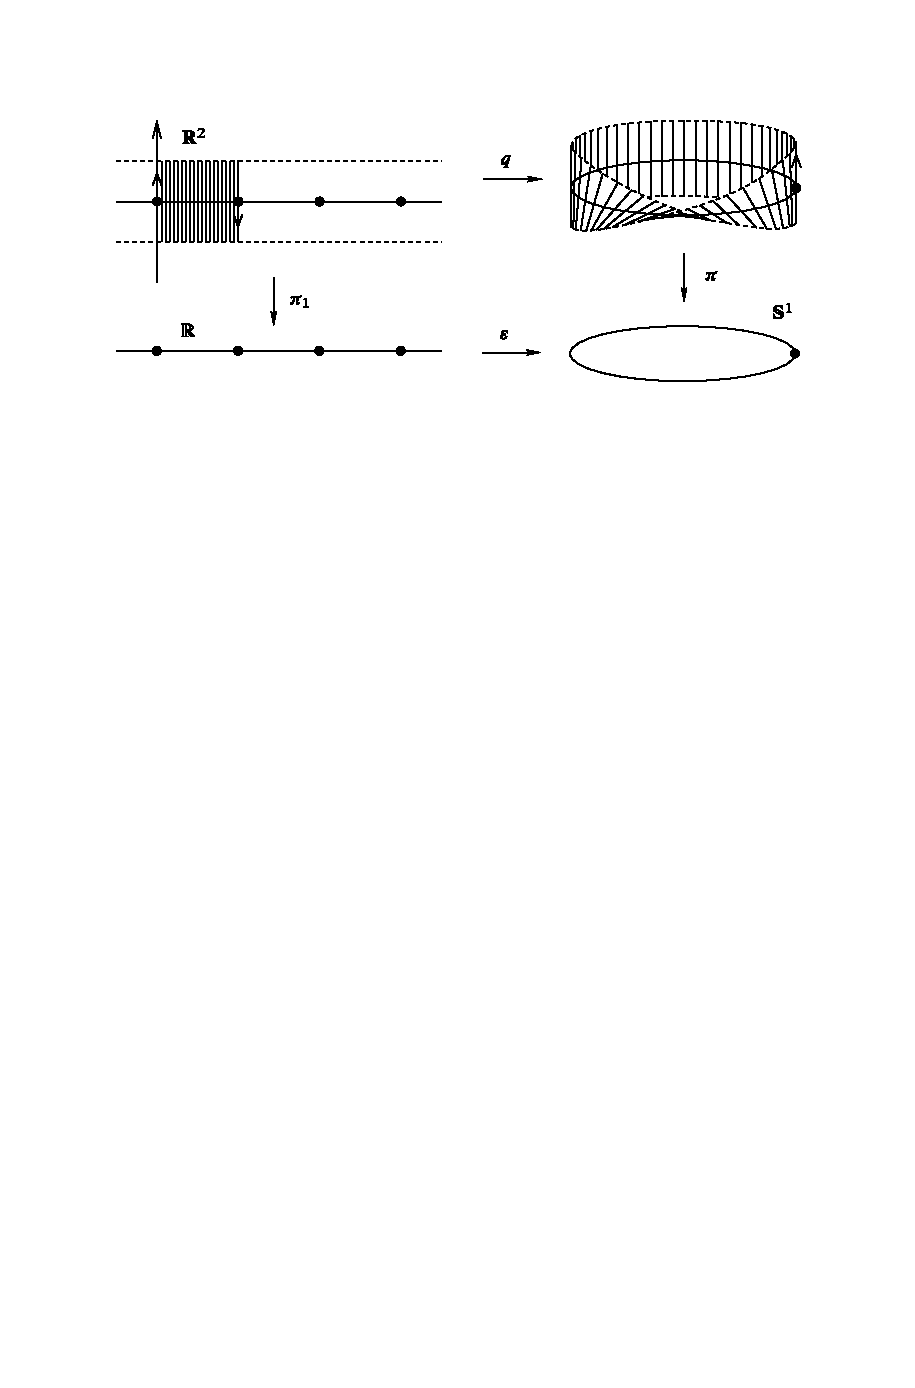
\includegraphics{Mobious-bundle}
\caption{Part of the Möbius bundle.}
\end{figure}\par
Consider the following commutative diagram:
\[\begin{tikzcd}
\R^2\ar[r,"q"]\ar[d,swap,"\pi_1"]&E\ar[d,dashed,"\pi"]\\
\R\ar[r,"\eps"]&S^1
\end{tikzcd}\]
where $\pi_1$ is the projection onto the first factor and $\eps:\R\to S^1$ is the smooth covering map $\eps(x)=e^{2\pi ix}$. Because $\eps\circ\pi_1$ is constant on each equivalence class, it descends to a continuous map $\pi:E\to S^1$. A straightforward verification shows that $E$ has a unique smooth manifold structure such that $q$ is a smooth covering map. and $\pi:E\to S^1$ is a smooth real line bundle over $S^1$, called the \textbf{M\"obius bundle}. $($If $U\sub S^1$ is an open subset that is evenly covered by $\eps$, and $\widetilde{U}\sub\R$ is a component of $\eps^{-1}(U)$, then $q$ restricts to a homeomorphism from $\widetilde{U}\times\R$ to $\pi^{-1}(U)$. Using this, one can construct a homeomorphism from $\pi^{-1}(U)$ to $U\times\R$, which serves as a local trivialization of $E$. These local trivializations can be interpreted as coordinate charts defining the smooth structure on $E$.$)$
\end{example}
The most important examples of vector bundles are tangent bundles.
\begin{proposition}[\textbf{The Tangent Bundle as a Vector Bundle}]\label{tangent bundle as vector bundle}
Let $M$ be a smooth $n$-manifold with or without boundary, and let $TM$ be its tangent bundle. With its standard projection map, its natural vector space structure on each fiber, and the topology and smooth structure constructed in Proposition~\ref{tangent bundle struct}, $TM$ is a smooth vector bundle of rank $n$ over $M$.
\end{proposition}
\begin{proof}
Given any smooth chart $(U,\varphi)$ for $M$ with coordinate functions $(x^i)$, define a map $\varPhi:\pi^{-1}(U)\to U\times\R^n$ by
\[\varPhi\Big(v^i\frac{\partial}{\partial x^i}\Big|_p\Big)=(p,(v^1,\dots,v^n))\]
This is linear on fibers and satisfies $\pi_U\circ\varPhi=\pi$. The composite map
\[\begin{tikzcd}
\pi^{-1}(U)\ar[r,"\varPhi"]&U\times\R^n\ar[r,"\varphi\times\mathrm{id}_{\R^n}"]&\varphi(U)\times\R^n
\end{tikzcd}\]
is equal to the coordinate map $\widetilde{\varphi}$ constructed in Proposition~\ref{tangent bundle struct}. Since both $\widetilde{\varphi}$ and $\varphi\times\mathrm{id}_{\R^n}$ are diffeomorphisms, so is $\varPhi$. Thus, $\varPhi$ satisfies all the conditions for a smooth local trivialization.
\end{proof}
Any bundle that is not trivial, of course, requires more than one local trivialization. The next lemma shows that the composition of two smooth local trivializations has a simple form where they overlap.
\begin{lemma}\label{vector bundle trivialization overlap}
Let $\pi:E\to M$ be a smooth vector bundle of rank $k$ over $M$. Suppose $\varPhi:\pi^{-1}(U)\to U\times\R^k$ and $\varPsi:\pi^{-1}(V)\to V\times\R^k$ are two smooth local trivializations of $E$ with $U\cap V=\emp$. There exists a smooth map $\tau:U\cap V\to\GL_k(\R)$ such that the composition $\varPhi\circ\varPsi^{-1}:(U\cap V)\times\R^k\to(U\cap V)\times\R^k$ has the form
\[\varPhi\circ\varPsi^{-1}(p,v)=(p,\tau(p)v)\]
where $\tau(p)v$ denotes the usual action of the $k\times k$ matrix $\tau(p)$ on the vector $v\in\R^k$.
\end{lemma}
\begin{proof}
The following diagram commutes:
\[\begin{tikzcd}
(U\cap V)\times\R^k\ar[rd,swap,"\pi_1"]&\pi^{-1}(U\cap V)\ar[l,swap,"\varPsi"]\ar[r,"\varPhi"]\ar[d,"\pi"]&(U\cap V)\times\R^k\ar[ld,"\pi_1"]\\
&U\cap V&
\end{tikzcd}\]
where the maps on top are to be interpreted as the restrictions of $\varPsi$ and $\varPhi$ to $\pi^{-1}(U\cap V)$. It follows that $\pi_1\circ(\varPhi\circ\varPsi^{-1})=\pi_1$, which means that
\[\varPhi\circ\varPsi^{-1}(p,v)=(p,\sigma(p,v))\]
for some smooth map $\sigma:(U\cap V)\times\R^k\to\R^k$. Moreover, for each fixed $p\in U\cap V$, the map $v\mapsto\sigma(p,v)$ from $\R^k$ to itself is an invertible linear map, so there is a nonsingular $k\times k$ matrix $\tau(p)$ such that $\sigma(p,v)=\tau(p)v$. If we choose a basis $(e_j)$ for $\R^k$ and let $\pi^i:\R^k\to\R$ be the projection on the $i$-th coordinate, then
\[\pi^i\circ\pi_2\circ\varPhi\circ\varPsi^{-1}(p,e_j)=\pi^i(\tau(p)e_j)=\pi^i(\tau^1_j(p)e_1+\cdots+\tau^k_j(p)e_k)=\tau^i_j(p)\]
so each function $\tau^i_j$ is a composition of smooth functions, hence is smooth. Because the matrix entries form global smooth coordinates for $\GL_k(\R)$, this implies that $\tau$ is smooth.
\end{proof}
The smooth map $\tau:U\cap V\to\GL_k(\R)$ described in this lemma is called the \textbf{transition function} between the local trivializations $\varPhi$ and $\varPsi$. For example, if $M$ is a smooth manifold and $\varPhi$ and $\varPsi$ are the local trivializations of $TM$ associated with two different smooth charts, then $(\ref{coordinate change-1})$ shows that the transition function between them is the Jacobian matrix of the coordinate transition map.\par
Like the tangent bundle, vector bundles are often most easily described by giving a collection of vector spaces, one for each point of the base manifold. In order to make such a set into a smooth vector bundle, we would first have to construct a manifold topology and a smooth structure on the disjoint union of all the vector spaces, 
and then construct the local trivializations and show that they have the requisite properties. The next lemma provides a shortcut, by showing that it is sufficient to construct the local trivializations, 
as long as they overlap with smooth transition functions.
\begin{lemma}[\textbf{Vector Bundle Chart Lemma}]\label{vector bundle chart lemma}
Let $M$ be a smooth manifold with or without boundary, and suppose that for each $p\in M$ we are given a real vector space $E_p$ of some fixed dimension $k$. Let $E=\coprod_{p\in M}E_p$ and let $\pi:E\to M$ be the map that takes each element of $E_p$ to the point $p$. Suppose furthermore that we are given the following data:
\begin{itemize}
\item[$(\rmnum{1})$] An open cover $\{U_\alpha\}_{\alpha\in A}$ of $M$.
\item[$(\rmnum{2})$] For each $\alpha\in A$, a bijective map $\varPhi_\alpha:\pi^{-1}(U_\alpha)\to U_\alpha\times\R^k$ whose restriction to each $E_p$ is a vector space isomorphism from $E_p$ to $\{p\}\times\R^k$.
\item[$(\rmnum{3})$] For each $\alpha,\beta\in A$ with $U_\alpha\cap U_\beta\neq\emp$, a smooth map $\tau_{\alpha\beta}:U_\alpha\cap U_\beta\to\GL_k(\R)$ such that the map $\varPhi_\alpha\circ\varPhi_\beta^{-1}$ from $(U_\alpha\cap U_\beta)\times\R^k$ to itself has the form
\begin{align}\label{vector bundle transition function-1}
\varPhi_\alpha\circ\varPhi_\beta^{-1}(p,v)=(p,\tau_{\alpha\beta}(p)v)
\end{align}
\end{itemize}
Then $E$ has a unique topology and smooth structure making it into a smooth manifold with or without boundary and a smooth rank-$k$ vector bundle over $M$, with $\pi$
as projection and $\{(U_\alpha,\varPhi_\alpha)\}$ as smooth local trivializations.
\end{lemma}
\begin{proof}
For each point $p\in M$, choose some $U_\alpha$ containing $p$, choose a smooth chart $(V_p,\varphi_p)$ for $M$ such that $p\in V_p\sub U_\alpha$ and let $\widehat{V}=\varphi_p(V_p)\sub\R^n$ or $\H^n$ (where $n$ is the dimension of $M$). Define a map $\widetilde{\varphi}_p:\pi^{-1}(V_p)\to\widehat{V}_p\times\R^k$ by $\widetilde{\varphi}_p=(\varphi_p\times\mathrm{id}_{\R^k})\circ\varPhi_\alpha$:
\[\begin{tikzcd}
\pi^{-1}(V_p)\ar[r,"\varPhi_\alpha"]&V_p\times\R^k\ar[rr,"\varphi_p\times\mathrm{id}_{\R^k}"]&&\widehat{V}_p\times\R^k
\end{tikzcd}\]
We will show that the collection of all such charts $\{(\pi^{-1}(V_p),\widetilde{\varphi}_p)\}$ satisfies the conditions of the smooth manifold chart lemma or its counterpart for manifolds with boundary, and therefore gives $E$ the structure of a smooth manifold with or without boundary.\par
As a composition of bijective maps, $\widetilde{\varphi}_p$ is bijective onto an open subset of either $\R^n\sub\R^k=\R^{n+k}$ or $\H^n\times\R^k=\H^{n+k}$. For any $p,q\in M$, it is easy to check that
\[\widetilde{\varphi}_p\big(\pi^{-1}(V_p)\cap\pi^{-1}(V_q)\big)=\varphi_p(V_p\cap V_q)\times\R^k\]
which is open because $\varphi_p$ is a homeomorphism onto an open subset of $\R^n$ or $\H^n$. Wherever two such charts overlap, we have
\[\widetilde{\varphi}_p\circ\widetilde{\varphi}_q^{-1}=(\varphi_p\times\mathrm{id}_{\R^k})\circ\varPhi_\alpha\circ\varPhi_\beta^{-1}\circ(\varphi_q\times\mathrm{id}_{\R^k})^{-1}\]
This composition is still a diffeomorphism, thus conditions $(\rmnum{1}),(\rmnum{2})$ and $(\rmnum{3})$ of Lemma~\ref{smooth mani chart lem} are satisfied. Because the open cover $\{V_p:p\in M\}$ has a countable subcover, $(\rmnum{4})$ is satisfied as well.\par
To check the Hausdorff condition $(\rmnum{5})$, just note that any two points in the same space $E_p$ lie in one of the charts we have constructed, while if $\xi\in E_p$ and $\eta\in E_q$ with $p\neq q$, we can choose $V_p$ and $V_q$ to be disjoint neighborhoods of $p$ and $q$, so that the sets $\pi^{-1}(V_p)$ and $\pi^{-1}(V_q)$ are disjoint coordinate neighborhoods containing $\xi$ and $\eta$, respectively. Thus we have given $E$ the structure of a smooth manifold with or without boundary.\par
With respect to this structure, each of the maps $\varPhi_\alpha$ is a diffeomorphism, because in terms of the coordinate charts $(\pi^{-1}(V_p),\widetilde{\varphi}_p)$ for $E$ and $(V_p\times\R^k,\varphi\times\mathrm{id}_{\R^k})$ for $V_p\times\R^k$, the coordinate representation of $\varPhi_\alpha$ is the identity map. The coordinate representation of $\pi$, with respect to the same chart for $E$ and the chart $(V_p,\varphi_p)$ for $M$, is $\pi(x,v)=x$, so $\pi$ is smooth as well. Because each $\varPhi_\alpha$ maps $E_p$ to $\{p\}\times\R^k$, it is immediate that $\pi_1\circ\varPhi_\alpha=\pi$ and $\varPhi_\alpha$ is linear on fibers by hypothesis. Thus, $\varPhi_\alpha$ satisfies all the conditions for a smooth local trivialization.\par
The fact that this is the unique such smooth structure follows easily from the requirement that the maps $\varPhi_\alpha$ be diffeomorphisms onto their images: any smooth structure satisfying the same conditions must include all of the charts we constructed, so it is equal to this one.
\end{proof}
Here are some examples showing how the chart lemma can be used to construct new vector bundles from old ones.
\begin{example}[\textbf{Whitney Sums}]
Given a smooth manifold $M$ and smooth vector bundles $E'\to M$ and $E''\to M$ of ranks $k_1$ and $k_2$, respectively, we will construct a new vector bundle over $M$ called the \textbf{Whitney sum} of $E'$ and $E''$, whose fiber at each $p\in M$ is the direct sum $E'_p\oplus E''_p$. The total space is defined as $E'\oplus E''=\coprod_{p\in M}(E'_p\oplus E''_p)$, with the obvious projection $\pi:E'\oplus E''\to M$. For each $p\in M$, choose a neighborhood $U$ of $p$ small enough that there exist local trivializations $(U,\varPhi_1)$ of $E'$ and $(U,\varPhi_2)$ of $E''$, and define $\varPhi:\pi^{-1}(U)\to U\times\R^{k_1+k_2}$ by 
\[\varPhi(v_1,v_2)=\big(\pi(v_1),(\pi_{\R^{k_1}}\circ\varPhi_1(v_1),\pi_{\R^{k_2}}\circ\varPhi_2(v_2))\big)\]
Suppose we are given another such pair of local trivializations $(\widetilde{U},\widetilde{\varPhi}_1)$ and $(\widetilde{U},\widetilde{\varPhi}_2)$. Let $\tau_1:(U\cap\widetilde{U})\to\GL_{k_1}(\R)$ and $\tau_2:(U\cap\widetilde{U})\to\GL_{k_2}(\R)$ be the corresponding transition functions. Then the transition function for $E'\oplus E''$ has the form
\[\widetilde{\varPhi}\circ\varPhi^{-1}(p,(v_1,v_2))=(p,\tau(p)(v_1,v_2))\]
where $\tau(p)=\tau_1(p)\oplus\tau_2(p)$ is the block diagonal matrix
\[\begin{pmatrix}
\tau_1(p)&0\\
0&\tau_2(p)
\end{pmatrix}\]
Because this depends smoothly on $p$, it follows from the chart lemma that $E'\oplus E''$ is a smooth vector bundle over $M$.
\end{example}
\begin{example}[\textbf{Restriction of a Vector Bundle}]
Suppose $\pi:E\to M$ is a rank-$k$ vector bundle and $S\sub M$ is any subset. We define the restriction of $E$ to $S$ to be the set $E|_S=\bigcup_{p\in S}E_p$, with the projection $E|_S\to S$ obtained by restricting $\pi$. If $\varPhi:\pi^{-1}(U)\to U\times\R^k$ is a local trivialization of $E$ over $U\sub M$, it restricts to a bijective map $\varPhi|_U:(\pi|_S)^{-1}(U\cap S)\to (U\cap S)\times\R^k$, and it is easy to check that these form local trivializations for a vector bundle structure on $E|_S$. If $E$ is a smooth vector bundle and $S\sub M$ is an embedded submanifold, it follows easily from the chart lemma that $E|_S$ is a smooth vector bundle.\par 
However, if $S$ is merely immersed, since the topology of $S$ is not the subspace topology, our argument above falis. Instead, we give $E|_S$ a topology and smooth structure making it into a smooth rank-$k$ vector bundle over $S$ as follows: For each $p\in S$, choose a neighborhood $U$ of $p$ in $M$ over which there is a local trivialization $\varPhi$ of $E$, and a neighborhood $V$ of $p$ in $S$ that is embedded in $M$ and contained in $U$. Then the restriction of $\varPhi$ to $\pi^{-1}(V)$ is a bijection from $\pi^{-1}(V)$ to $V\times\R^k$, and we can apply the chart lemma to these bijections to yield the desired structure.
\end{example}
Now we use the chart lemma to give another way to construct a vector bundle. First we need an observation.
\begin{lemma}\label{vector bundle cochain prop}
Let $\pi:E\to M$ be a smooth vector bundle of rank $k$ over a smooth manifold $M$ with or without boundary. Suppose that $\{U_\alpha\}_{\alpha\in A}$ is an open 
cover of $M$, and for each $\alpha\in A$ we are given a smooth local trivialization $\varPhi_\alpha:\pi^{-1}(U_\alpha)\to U_\alpha\times\R^k$ of $E$. For 
each $\alpha,\beta\in A$ such that $U_\alpha\cap U_\beta\neq\emp$, let $\tau_{\alpha\beta}:U_{\alpha}\cap U_{\beta}\to\GL_k(\R)$ be the transition function 
defined by $(\ref{vector bundle transition function-1})$. Then the following identity is satisfied for all $\alpha,\beta,\gamma\in A$:
\begin{align}\label{vector bundle transition function-2}
\tau_{\alpha\beta}(p)\tau_{\beta\gamma}(p)=\tau_{\alpha\gamma}(p),\quad p\in U_\alpha\cap U_\beta\cap U_\gamma,
\end{align}
where the juxtaposition on the left-hand side represents matrix multiplication and $\tau_{\alpha\alpha}=I_k$ for all $\alpha\in A$.
\end{lemma}
\begin{proof}
By definition we have
\begin{align*}
\varPhi_\alpha\circ\varPhi_{\beta}^{-1}(p,v)=(p,\tau_{\alpha\beta}(p)v).
\end{align*}
Thus fix a $p\in U_\alpha\cap U_\beta\cap U_\gamma$, we get
\[(\tau_{\alpha\beta}(p)\tau_{\beta\gamma}(p)v)=\varPhi_\alpha\circ\varPhi_{\beta}^{-1}\circ\varPhi_\beta\circ\varPhi_{\gamma}^{-1}(p,v)=\varPhi_{\alpha}\circ\varPhi_{\gamma}(p,v)=(p,\tau_{\alpha\gamma}v)\]
Since this holds for all $v\in E_p$, we conclude $\tau_{\alpha\beta}(p)\tau_{\beta\gamma}(p)=\tau_{\alpha\gamma}(p)$.
\end{proof}
\begin{theorem}[\textbf{Vector bundle construction theorem}]\label{vector bundle construct}
Let $M$ be a smooth manifold with or without boundary, and let $\{U_\alpha\}_{\alpha\in A}$ be an open cover of $M$. Suppose for each $\alpha,\beta\in A$ we are 
given a smooth map $\tau_{\alpha\beta}:U_{\alpha}\cap U_{\beta}\to\GL_k(\R)$ such that $(\ref{vector bundle transition function-2})$ is satisfied for all $\alpha,\beta,\gamma\in A$. 
Then there is a smooth rank-$k$ vector bundle $\pi:E\to M$ with smooth local trivializations $\varPhi_\alpha:\pi^{-1}(U_\alpha)\to U_\alpha\times\R^k$ whose transition functions are the given maps $\tau_{\alpha\beta}$.
\end{theorem}
\begin{proof}
Define an equivalence relation on $\coprod_{\alpha\in A}(U_\alpha\times\R^k)$: for $(p_1,v_1)\in U_\alpha\times\R^k$ and $(p_2,v_2)\in U_\beta\times\R^k$,
\[(p_1,v_1)\sim(p_2,v_2)\iff p_1=p_2\And v_1=\tau_{\alpha\beta}(p_2)v_2.\]
This is well defined in view of $(\ref{vector bundle transition function-2})$:
\begin{itemize}
\item Since $\tau_{\alpha\alpha}(p)=I_k$, we have $(p,v)\sim(p,v)$ for all $(p,v)$.
\item If $v_1=\tau_{\alpha\beta}(p)v_2$, then $v_2=\tau_{\beta\alpha}(p)v_1$, since $\tau_{\alpha\beta}\tau_{\beta\alpha}=\tau_{\alpha\alpha}=\mathrm{id}$.
\item If $v_1=\tau_{\alpha\beta}(p)v_2$ and $v_2=\tau_{\beta\gamma}(p)v_3$, then $v_1=\tau_{\alpha\beta}(p)\tau_{\beta\gamma}(p)v_2=\tau_{\alpha\gamma}(p)v_3$.
\end{itemize}
Thus we can form the quotient space $E:=\coprod_{\alpha\in A}(U_\alpha\times\R^k)/\sim$. We define a map $\pi:E\to M$ by
\[\pi(p,v)=p\]
so that $\pi^{-1}(U_\alpha)$ is the equivalent class of $U_\alpha\times\R^k$. Now define a local trivalization $\varPhi_\alpha:\pi^{-1}(U_\alpha)\to U_\alpha\times\R^k$ by $\varPhi_\alpha(p,v)=(p,v)$. We can check, by our equivalent relation: for $(p,v)\in U_\beta\times\R^k$,
\[\varPhi_\alpha\circ\varPhi_\beta^{-1}(p,v)=\{(p,v')\in U_\alpha\times\R^k:v'=\tau_{\alpha\beta}(p)v\}=(p,\tau_{\alpha\beta}(p)v)\]
Thus by the chart lemma, $\pi:E\to M$ is a vector bundle.
\end{proof}
\subsection{Sections of vector bundles}
Let $\pi:E\to M$ be a vector bundle. A \textbf{section} of $E$ (sometimes called a \textbf{cross section}) is a section of the map $\pi$, that is, a continuous map $\sigma:M\to E$ satisfying $\pi\circ\sigma=\mathrm{id}_M$. This means that $\sigma(p)$ is an element of the fiber $E_p$ for each $p\in M$.\par
More generally, a \textbf{local section} of $E$ is a continuous map $\sigma:U\to E$ defined on some open subset $U\sub M$ and satisfying $\pi\circ\sigma=\mathrm{id}_U$. To emphasize the distinction, a section defined on all of $M$ is sometimes called a \textbf{global section}. Note that a local section of $E$ over $U\sub M$ is the same as a global section of the restricted bundle $E|_U$. If $M$ is a smooth manifold with or without boundary and $E$ is a smooth vector bundle, a \textbf{smooth (local or global) section} of $E$ is one that is a smooth map from its domain to $E$.\par
Just as with vector fields, for some purposes it is useful also to consider maps that would be sections except that they might not be continuous. Thus, we define a \textbf{rough (local or global) section} of $E$ over a set $U\sub M$ to be a map $\sigma:U\to E$ (not necessarily continuous) such that $\pi\circ\sigma=\mathrm{id}_U$. A section without further qualification always means a continuous section.\par
The \textbf{zero section} of $E$ is the global section $\zeta:M\to E$ defined by
\[\zeta(p)=0\in E_p\quad\text{for each }p\in M.\]
As in the case of vector fields, the \textbf{support} of a section $\sigma$ is the closure of the set $\{p\in M:\sigma(p)\neq 0\}$.
\begin{example}[\textbf{Sections of Vector Bundles}]
Suppose $M$ is a smooth manifold with or without boundary.
\begin{itemize}
\item[(a)]Sections of $TM$ are vector fields on $M$.
\item[(b)]Given an immersed submanifold $S\sub M$ with or without boundary, a section of the ambient tangent bundle $TM|_S\to S$ is called a \textbf{vector field along $\bm{S}$}. It is a continuous map $X:S\to TM$ such that $X_p\in T_pM$ for each $p\in S$. This is different from a vector field on $S$, which satisfies $X_p\in T_pS$ at each point.
\item[(c)]If $E=M\times\R^k$ is a product bundle, there is a natural one-to-one correspondence between sections of $E$ and continuous functions from $M$ to $\R^k$: a continuous function $F:M\to\R^k$ determines a section $\widetilde{F}:M\to M\times\R^k$ by $\widetilde{F}(x)=(x,F(x))$, and vice versa. If $M$ is a smooth manifold with or without boundary, then the section $\widetilde{F}$ is smooth if and only if $F$ is.
\item[(d)]The correspondence in the preceding paragraph yields a natural identification between the space $C^\infty(M)$ and the space of smooth sections of the trivial line bundle $M\times\R\to M$.
\end{itemize}
\end{example}
If $E\to M$ is a smooth vector bundle, the set of all smooth global sections of $E$ is a vector space under pointwise addition and scalar multiplication:
\[(c_1\sigma_1+c_2\sigma_2)(p)=c_1\sigma_1(p)+c_2\sigma_2(p)\]
This vector space is usually denoted by $\Gamma(E)$. Just like smooth vector fields, smooth sections of a smooth bundle $E\to M$ can be multiplied by smooth real-valued functions: if $f\in C^\infty(M)$ and $\sigma\in\Gamma(E)$, we obtain a new section $f\sigma$ defined by
\[(f\sigma)(p)=f(p)\sigma(p)\]
\begin{lemma}[\textbf{Extension Lemma for Vector Bundles}]\label{ext lem vector bundle}
Let $\pi:E\to M$ be a smooth vector bundle over a smooth manifold $M$ with or without boundary.
\begin{itemize}
\item[(a)] Suppose $A$ is a closed subset of $M$ and $\sigma:A\to E$ is a section of $E|_A$ that is smooth in the sense that $\sigma$ extends to a smooth local section of $E$ in a neighborhood of each point. For each open subset $U\sub M$ containing $A$, there exists a global smooth section $\widetilde{\sigma}\in\Gamma(E)$ such that $\widetilde{\sigma}|_A=\sigma$ and $\supp(\widetilde{\sigma})\sub U$.
\item[(b)]Suppose $S\sub M$ is an embedded submanifold with or without boundary. For any smooth section $\sigma$ of the restricted bundle $E|_S\to S$, there exist a neighborhood $U$ of $S$ in $M$ and a smooth section $\widetilde{\sigma}$ of $E|_U$ such that $\widetilde{\sigma}|_S=\sigma$. If $E$ has positive rank, then every smooth section of $E|_S$ extends smoothly to all of $M$ if and only if $S$ is properly embedded.
\end{itemize}
\end{lemma}
\begin{proof}
See Lemma~\ref{ext lem smooth func}.
\end{proof}
\subsubsection{Local and global frames}
Let $E\to M$ be a vector bundle. If $U\sub M$ is an open subset, a $k$-tuple of local sections $(\sigma_1,\dots,\sigma_k)$ of $E$ over $U$ is said to be \textbf{linearly independent} if their values $(\sigma_1(p),\dots,\sigma_k(p))$ form a linearly independent $k$-tuple in $E_p$ for each $p\in U$. Similarly, they are said to \textbf{span $\bm{E}$} if their values span $E_p$ for each $p\in U$. A \textbf{local frame} for $E$ over $U$ is an ordered $k$-tuple $(\sigma_1,\dots,\sigma_k)$ of linearly independent local sections over $U$ that span $E$; thus $(\sigma_1(p),\dots,\sigma_k(p))$ is a basis for the fiber $E_p$ for each $p\in U$. It is called a \textbf{global frame} if $U=M$. If $E\to M$ is a smooth vector bundle, a local or global frame is a \textbf{smooth frame} if each $\sigma_i$ is a smooth section. We often denote a frame $(\sigma_1,\dots,\sigma_k)$ by $(\sigma_i)$.\par
The next proposition is an analogue for vector bundles of Proposition~\ref{local frame completion}.
\begin{proposition}[\textbf{Completion of Local Frames for Vector Bundles}]\label{vector bundle local frame completion}
Suppose $\pi:E\to M$ is a smooth vector bundle of rank $k$.
\begin{itemize}
\item[(a)] If $(\sigma_1,\dots,\sigma_m)$ is a linearly independent $m$-tuple of smooth local sections of $E$ over an open subset $U\sub M$, with $1\leq m<k$, then for each $p\in U$ there exist smooth sections $\sigma_{m+1},\dots,\sigma_k$ defined on some neighborhood $V$ of $p$ such that $(\sigma_1,\dots,\sigma_k)$ is a smooth local frame for $E$ over $U\cap V$.
\item[(b)] If $(v_1,\dots,v_m)$ is a linearly independent $m$-tuple of elements of $E_p$ for some $p\in M$, with $1\leq m\leq k$, then there exists a smooth local frame $(\sigma_i)$ for $E$ over some neighborhood of $p$ such that $\sigma_i(p)=v_i$ for $i=1,\dots,m$.
\item[(c)] If $A\sub M$ is a closed subset and $(\tau_1,\dots,\tau_k)$ is a linearly independent $k$-tuple of sections of $E|_A$ that are smooth in the sense described in Lemma~\ref{ext lem vector bundle}, then there exists a smooth local frame $(\sigma_1,\dots,\sigma_k)$ for $E$ over some neighborhood of $A$ such that $\sigma_i|_A=\tau_i$ for $i=1,\dots,k$.
\end{itemize}
\end{proposition}
Local frames for a vector bundle are intimately connected with local trivializations, as the next two examples show.
\begin{example}[\textbf{A Global Frame for a Product Bundle}]
If $E=M\times\R^k$ is a product bundle, the standard basis $(e_1,\dots,e_k)$ for $\R^k$ yields a global frame $(\widetilde{e}_i)$ for $E$, defined by $\widetilde{e}_i(p)=(p,e_i)$. If $M$ is a smooth manifold with or without
boundary, then this global frame is smooth.
\end{example}
\begin{example}[\textbf{Local Frames Associated with Local Trivializations}]\label{local frame trivialization}
Suppose $\pi:E\to M$ is a smooth vector bundle. If $\varPhi:\pi^{-1}(U)\to U\times\R^k$ is a smooth local trivialization of $E$, we can use the same idea as in the preceding example to construct a local frame for $E$ over $U$. Define maps $\sigma_1,\dots,\sigma_k:U\to E$ by $\sigma_i(p)=\varPhi^{-1}(p,e_i)=\varPhi^{-1}\circ\widetilde{e}_i(p)$:
\[\begin{tikzcd}
\pi^{-1}(U)\ar[rd,"\pi"]\ar[rr,"\varPhi"]&&U\times\R^k\ar[ld,swap,"\pi_1"]\\
&U\ar[lu,bend left=35,"\sigma_i"]\ar[ru,bend right=35,swap,"\widetilde{e}_i"]&
\end{tikzcd}\]
Then $\sigma_i$ is smooth because $\varPhi$ is a diffeomorphism, and the fact that $\pi_1\circ\varPhi=\pi$ implies that
\[\pi\circ\sigma_i(p)=\pi\circ\varPhi^{-1}(p,e_i)=\pi_1(p,e_i)=p,\]
so $\sigma_i$ is a section. To see that $(\sigma_i(p))$ forms a basis for $E_p$, just note that $\varPhi$ restricts to an isomorphism from $E_p$ to $\{p\}\times\R^k$, and $\varPhi(\sigma_i(p))=(p,e_i)$, so $\varPhi$ takes $(\sigma_i(p))$ to the standard basis for $\{p\}\times\R^k\cong\R^k$. We say that this local frame $(\sigma_i)$ is \textbf{associated with $\bm{\varPhi}$}.
\end{example}
\begin{proposition}\label{local frame iff trivialization}
Every smooth local frame for a smooth vector bundle is associated
with a smooth local trivialization as in Example~\ref{local frame trivialization}.
\end{proposition}
\begin{proof}
Suppose $E\to M$ is a smooth vector bundle and $(\sigma_i)$ is a smooth local frame for $E$ over an open subset $U\sub M$. We define a map $\varPsi:U\times\R^k\to\pi^{-1}(U)$ by
\[\varPsi(p,(v^1,\dots,v^k))=v^i\sigma_i(p).\]
The fact that $\sigma_i(p)$ forms a basis for $E_p$ at each $p\in U$ implies that $\varPsi$ is bijective, and an easy computation shows that $\sigma_i=\varPsi\circ\widetilde{e}_i$. Thus, if we can show that $\varPsi$ is
a diffeomorphism, then $\varPsi^{-1}$ will be a smooth local trivialization whose associated local frame is $(\sigma_i)$.\par
Since $\varPsi$ is bijective, to show that it is a diffeomorphism it suffices to show that it is a local diffeomorphism. Given $q\in U$, we can choose a neighborhood $V$ of $q$ in $M$ over which there exists a smooth local trivialization $\varPhi:\pi^{-1}(V)\to V\times\R^k$, and by shrinking $V$ if necessary we may assume that $V\sub U$. Since $\varPhi$ is a diffeomorphism, if we can show that $\varPhi\circ\varPsi|_{V\times\R^k}$ is a diffeomorphism from $V\times\R^k$ to itself, it follows that $\varPsi$ restricts to a diffeomorphism from $V\times\R^k$ to $V$:
\[\begin{tikzcd}
V\times\R^k\ar[rd,swap,"\pi_1"]\ar[r,"\varPsi|_{V\times\R^k}"]&\pi^{-1}(V)\ar[d,"\pi"]\ar[r,"\varPhi"]&V\times\R^k\ar[ld,"\pi_1"]\\
&V&
\end{tikzcd}\]
For each of our smooth sections $\sigma_i$, the composite map $\varPhi\circ\sigma_i|_V:V\to V\times\R^k$ is smooth, and thus there are smooth functions $\sigma_i^1,\dots,\sigma_i^k:V\to\R$
\[\varPhi\circ\sigma_i(p)=\big(p,(\sigma_i^1(p),\dots,\sigma_i^k(p))\big).\]
On $V\times\R^k$, therefore
\[\varPhi\circ\varPsi(p,(v^1,\dots,v^k))=\big(p,(v^i\sigma_i^1(p),\dots,v^i\sigma_i^k(p))\big),\]
which is clearly smooth.\par
To show that $(\varPhi\circ\varPsi)^{-1}$ is smooth, note that the matrix $(\sigma_i^j(p))$ is invertible for each $p$, because $(\sigma_i(p))$ is a basis for $E_p$. Let $(\tau_i^j(p))$ denote the inverse matrix. Because matrix inversion is a smooth map from $\GL_k(\R)$ to itself, the functions $\tau_i^j$ are smooth. It follows from the computations in the preceding paragraph that
\[(\varPhi\circ\varPsi)^{-1}(p,(w^1,\dots,w^k))=\big(p,(w^1\tau_i^1(p),\dots,w^k\tau_i^k(p))\big),\]
which is also smooth.
\end{proof}
\begin{corollary}
A smooth vector bundle is smoothly trivial if and only if it admits a smooth global frame.
\end{corollary}
\begin{proof}
Example~\ref{local frame trivialization} and Proposition~\ref{local frame iff trivialization} show that there is a smooth local trivialization over an open subset $U\sub M$ if and only if there is a smooth local frame over $U$. The corollary is just the special case of this statement when $U=M$.
\end{proof}
When applied to the tangent bundle of a smooth manifold $M$, this corollary says that $TM$ is trivial if and only if $M$ is parallelizable.
\begin{corollary}\label{vector bundle chart from frame}
Let $\pi:E\to M$ be a smooth vector bundle of rank $k$, let $(V,\varphi)$ be a smooth chart on $M$ with coordinate functions $(x^i)$, and suppose there exists a smooth local frame $(\sigma_i)$ for $E$ over $V$. Define $\widetilde{\varphi}:\pi^{-1}(V)\to\varphi(V)\times\R^k$ by
\[\widetilde{\varphi}(v^i\sigma_i(p))=(x^1(p),\dots,x^n(p),v^1,\dots,v^k).\]
Then $(\pi^{-1}(V),\widetilde{\varphi})$ is a smooth coordinate chart for $E$.
\end{corollary}
\begin{proof}
Just check that $\widetilde{\varphi}$ is equal to the composition $(\varphi\times\mathrm{id}_{\R^k})\circ\varPhi$, where $\varPhi$ is the local trivialization associated with $(\sigma_i)$. As a composition of diffeomorphisms, it is a diffeomorphism.
\end{proof}
Suppose $(\sigma_i)$ is a smooth local frame for $E$ over some open subset $U\sub M$. If $\tau:M\to E$ is a rough section, the value of $\tau$ at an arbitrary point $p\in U$ can be written $\tau(p)=\tau^i(p)\sigma_i(p)$ for some uniquely determined numbers $(\tau^1(p),\dots,\tau^n(p))$. This defines $k$ functions $\tau^i:U\to\R$, called the \textbf{component functions of $\bm{\tau}$} with respect to the given local frame.
\begin{proposition}[\textbf{Local Frame Criterion for Smoothness}]\label{local frame smooth crit}
Let $\pi:E\to M$ be a smooth vector bundle, and let $\tau:M\to E$ be a rough section. If $(\sigma_i)$ is a smooth local frame for $E$ over an open subset $U\sub M$, then $\tau$ is smooth on $U$ if and only if its component functions with respect to $(\sigma_i)$ are smooth.
\end{proposition}
\begin{proof}
Let $\varPhi:\pi^{-1}(U)\to U\times\R^k$ be the local trivialization associated with the local frame $\varPhi$. Because $\varPhi$ is a diffeomorphism, $\tau$ is smooth on $U$ if and only if the composite map $\varPhi\circ\tau$ is smooth on $U$. It is straightforward to check that $\varPhi\circ\tau(p)=\big(p,(\tau^1(p),\dots,\tau^k(p))\big)$ where $\tau^i$ are the component functions of $\tau$ with respect to $(\sigma_i)$, so $\varPhi\circ\tau$ is smooth if and only if the component functions $\tau^i$
are smooth.
\end{proof}
Proposition~\ref{local frame smooth crit} applies equally well to local sections, since a local section of $E$ over an open subset $V\sub M$ is a global section of the restricted bundle $E|_V$.\par
The correspondence between local frames and local trivializations leads to the
following uniqueness result characterizing the smooth structure on the tangent bundle of a smooth manifold.
\begin{proposition}[\textbf{Uniqueness of the Smooth Structure on $\bm{TM}$}]\label{tangent bundle struct unique}
Let $M$ be a smooth $n$-manifold with or without boundary. The topology and smooth structure on $TM$ constructed in Proposition~\ref{tangent bundle struct} are the 
unique ones with respect to which $\pi:TM\to M$ is a smooth vector bundle with the given vector space structure on the fibers, and such that all coordinate vector 
fields are smooth local sections.
\end{proposition}
\begin{proof}
Suppose $TM$ is endowed with some topology and smooth structure making it into a smooth vector bundle with the given properties. If $(U,\varphi)$ is any smooth chart for $M$, the corresponding coordinate frame $(\partial/\partial x^i)$ is a smooth local frame over $U$, so by Proposition~\ref{local frame iff trivialization} there is a smooth local trivialization $\varPhi:\pi^{-1}(U)\to U\times\R^k$ associated with this local frame, which, according to Example~\ref{local frame trivialization}, is defined by
\[\varPhi(v^i\frac{\partial}{\partial x^i}\Big|_p)=\big(p,(v^1,\dots,v^n)\big)\] But this is none other than the map we constructed in Proposition~\ref{tangent bundle as vector bundle}. It follows from Corollary~\ref{vector bundle chart from frame} that the natural coordinate chart $\widetilde{\varphi}=(\varphi\times\mathrm{id}_{\R^n})\circ\varPhi$ belongs to the given smooth structure. Thus, the given smooth structure is equal to the one constructed in Proposition~\ref{tangent bundle struct}.
\end{proof}
\subsection{Bundle homomorphisms}
If $\pi:E\to M$ and $\pi':E'\to M'$ are vector bundles, a continuous map $F:E\to E'$ is called a \textbf{bundle homomorphism} if there exists a map $f:M\to M'$ 
satisfying $\pi'\circ F=f\circ\pi$,
\[\begin{tikzcd}
E\ar[r,"F"]\ar[d,swap,"\pi"]&E'\ar[d,"\pi'"]\\
M\ar[r,"f"]&M'
\end{tikzcd}\]
with the property that for each $p\in M$, the restricted map $F|_{E_p}:E_p\to E'_{f(p)}$ is linear. The relationship between $F$ and $f$ is expressed by saying that 
$F$ covers $f$.
\begin{proposition}
Suppose $\pi:E\to M$ and $\pi':E'\to M'$ are vector bundles and $F:E\to E'$ is a bundle homomorphism covering $f:M\to M'$. Then $f$ is continuous and is uniquely determined by $F$. If the bundles and $F$ are all smooth, then $f$ is smooth as well.
\end{proposition}
\begin{proof}
All of the conclusions follow from the easily verified fact that $f=\pi'\circ F\circ\zeta$, where $\zeta:M\to E$ is the zero section.
\end{proof}
A bijective bundle homomorphism $F:E\to E'$ whose inverse is also a bundle homomorphism is called a \textbf{bundle isomorphism}; if $F$ is also a diffeomorphism, it is 
called a \textbf{smooth bundle isomorphism}. If there exists a (smooth) bundle isomorphism between $E$ and $E'$, the two bundles are said to be (smoothly) 
\textbf{isomorphic}. In the special case in which both $E$ and $E'$ are vector bundles over the same base space $M$, a slightly more restrictive notion of bundle 
homomorphism is usually more useful. A \textbf{bundle homomorphism over $\bm{M}$} is a bundle homomorphism covering the identity map of $M$, or in other words, 
a continuous map $F:E\to E'$ such that $\pi'\circ F=\pi$,
\[\begin{tikzcd}
E\ar[rr,"F"]\ar[rd,swap,"\pi"]&&E'\ar[ld,"\pi'"]\\
&M&
\end{tikzcd}\]
and whose restriction to each fiber is linear. If there exists a bundle homomorphism $F:E\to E'$ over $M$ that is also a (smooth) bundle isomorphism, then we say that $E$ and $E'$ are (smoothly) \textbf{isomorphic over $\bm{M}$}. The next proposition shows that it is not necessary to check smoothness of the inverse.
\begin{proposition}\label{vector bundle smooth iso iff bi}
Suppose $E$ and $E'$ are smooth vector bundles over a smooth manifold $M$ with or without boundary, and $F:E\to E'$ is a bijective smooth bundle homomorphism over $M$. Then $F$ is a smooth bundle isomorphism.
\end{proposition}
\begin{proof}
Since $\pi$ and $\pi'$ are both local diffeomorphisms, it follows that $F$ is also a local diffeomorphisms. Now a local diffeomorphisms is a diffeomorphisms if and only if it is bijective.
\end{proof}
\begin{corollary}
A smooth rank-$k$ vector bundle over $M$ is smoothly trivial if and only if it is smoothly isomorphic over $M$ to the product bundle $M\times\R^k$.
\end{corollary}
\begin{proof}
A smooth rank-$k$ vector bundle $\pi:E\to M$ is smoothly trivial if and only if it admits a global trivialization $\varPhi:E\to M\times\R^k$. Note that, by definition $\pi\circ\varPhi=\pi$, that is, it is a bundle homomorphism. Now the claim is obvious.
\end{proof}
\begin{example}[\textbf{Bundle Homomorphisms}]
\mbox{}
\begin{itemize}
\item[(a)]If $F:M\to N$ is a smooth map, the global differential $dF:TM\to TN$ is a smooth bundle homomorphism covering $F$.
\item[(b)]If $E\to M$ is a smooth vector bundle and $S\sub M$ is an immersed submanifold with or without boundary, then the inclusion map $E|_S\hookrightarrow E$ is a smooth bundle homomorphism covering the inclusion of $S$ into $M$.
\end{itemize}
\end{example}
Suppose $E\to M$ and $E'\to M$ are smooth vector bundles over a smooth manifold $M$ with or without boundary, and let $\Gamma(E)$, $\Gamma(E')$ denote their spaces of smooth global sections. If $F:E\to E'$ is a smooth bundle homomorphism over $M$, then composition with $F$ induces a map $\widetilde{F}:\Gamma(E)\to\Gamma(E')$ as follows:
\begin{align}\label{global section homomorphism-1}
\widetilde{F}(\sigma)(p)=(F\circ\sigma)(p)=F(\sigma(p))
\end{align}
It is easy to check that $\widetilde{F}$ is a section of $E'$, and it is smooth by composition.\par
Because a bundle homomorphism is linear on fibers, the resulting map $\widetilde{F}$ on sections is linear over $\R$. In fact, it satisfies a stronger linearity 
property. A map $\mathcal{F}:\Gamma(E)\to\Gamma(E')$ is said to be \textbf{linear over $\bm{C^\infty(M)}$} if for any smooth functions $u_1,u_2\in C^\infty(M)$ and 
smooth sections $\sigma_1,\sigma_2\in\Gamma(E)$,
\[\mathcal{F}(u_1\sigma_1+u_2\sigma_2)=u_1\mathcal{F}(\sigma_1)+u_2\mathcal{F}(\sigma_2)\]
That is, $\mathcal{F}$ is a $C^\infty(M)$-module homomorphism. It follows easily from the linearity of $F$ on each $E_p$ that the map on sections induced by a smooth 
bundle homomorphism is linear over $C^\infty(M)$. It turns out that the converse is true as well. To prove this, we first introduce some terminologies.
\begin{definition}
Let $E$ and $E'$ be vector bundles over a manifold $M$. An $\R$-linear map $\mathcal{F}:\Gamma(E)\to\Gamma(F)$ is a \textbf{local operator} if whenever a section 
$s\in\Gamma(E)$ vanishes on an open set $U$ in $M$, then $\mathcal{F}(s)\in\Gamma(F)$ also vanishes on $U$. It is a \textbf{point operator} if whenever a section 
$s\in\Gamma(E)$ vanishes at a point $p$ in $M$, then $\mathcal{F}(s)\in\Gamma(F)$ also vanishes at $p$.
\end{definition}
\begin{lemma}\label{vector bundle section map pointwise}
Let $E$ and $E'$ be smooth vector bundles over a manifold $M$. If a map $\mathcal{F}:\Gamma(E)\to\Gamma(E')$ is $C^{\infty}(M)$-linear, then it is a point operator.
\end{lemma}
\begin{proof}
First, we show that $\mathcal{F}$ acts locally: if $\sigma_1\equiv\sigma_2$ in some open subset $U\sub M$, then $\mathcal{F}(\sigma_1)\equiv\mathcal{F}(\sigma_2)$ in 
$U$. Write $\tau=\sigma_1-\sigma_2$, then by linearity of $\mathcal{F}$, it suffices to assume that $\tau$ vanishes in $U$ and show that $\mathcal{F}(\tau)$ does too. 
Given $p\in U$, let $\psi\in C^\infty(M)$ be a smooth bump function supported in $U$ and equal to $1$ at $p$. Because $\psi\tau$ is identically zero on $M$, the fact 
that $\mathcal{F}$ is linear over $C^\infty(M)$ implies
\[0=\mathcal{F}(\psi\tau)=\psi\mathcal{F}(\tau).\]
Evaluating at $p$ shows that $\mathcal{F}(\tau)(p)=\psi(p)\mathcal{F}(\tau)(p)=0$; since the same is true for every $p\in U$, the claim follows.\par
Next we show that $\mathcal{F}$ actually acts pointwise: if $\sigma_1(p)=\sigma_2(p)$, then $\mathcal{F}(\sigma_1)(p)=\mathcal{F}(\sigma_2)(p)$. Once again, it suffices 
to assume that $\tau(p)=0$ and show that $\mathcal{F}(\tau)(p)=0$. Let $(\sigma_1,\dots,\sigma_k)$ be a smooth local frame for $E$ in some neighborhood $U$ of $p$, and 
write $\tau$ in terms of this frame as $\tau=u^i\sigma_i$ for some smooth functions $u^i$ defined in $U$. The fact that $\tau(p)=0$ means that $u^1(p)=\cdots=u^k(p)=0$. 
By the extension lemmas for vector bundles and for functions, there exist smooth global sections $\widetilde{\sigma}_i\in\Gamma(E)$ that agree with $\sigma_i$ in a 
neighborhood of $p$, and smooth functions $\widetilde{u}^i$ that agree with $u^i$ in some neighborhood of $p$. Then since $\tau=\widetilde{u}^i\widetilde{\sigma}_i$ on 
a neighborhood of $p$, we have
\[\mathcal{F}(\tau)(p)=\mathcal{F}(\widetilde{u}^i\widetilde{\sigma}_i)(p)=\widetilde{u}^i(p)\mathcal{F}(\widetilde{\sigma}_i)(p)=0.\]
Therefore $\mathcal{F}$ is a point operator.
\end{proof}
\begin{lemma}[\textbf{Bundle Homomorphism Characterization Lemma}]\label{vector bundle homo char}
Let $\pi:E\to M$ and $\pi:E'\to M$ be smooth vector bundles over a smooth manifold $M$ with or without boundary, and let $\Gamma(E),\Gamma(E')$ denote their spaces of 
smooth sections. A map $\mathcal{F}:\Gamma(E)\to\Gamma(E')$ is linear over $C^\infty(M)$ if and only if there is a smooth bundle homomorphism $F:E\to E'$ over $M$ such 
that $\mathcal{F}(\sigma)=F\circ\sigma$ for all $\sigma\in\Gamma(E)$.
\end{lemma}
\begin{proof}
We noted above that the map on sections induced by a smooth bundle homomorphism
is linear over $C^\infty(M)$. Conversely, suppose $\mathcal{F}:\Gamma(E)\to\Gamma(E')$ is linear over $C^\infty(M)$. By Lemma~\ref{vector bundle section map pointwise} 
we know that $\mathcal{F}$ is a point operator, so we can define a bundle homomorphism $F:E\to E'$ as follows. For any $p\in M$ and $v\in E_p$, let 
$F(v)=\mathcal{F}(\widetilde{v})(p)\in E'_p$, where $\widetilde{v}$ is any global smooth section of $E$ such that $\widetilde{v}(p)=v$. Since $\mathcal{F}$ is a point 
operator, the resulting element of $E'_p$ is independent of the choice of section. This map $F$ clearly satisfies $\pi'\circ F=\pi$, and it is linear on each fiber 
because of the linearity of $\mathcal{F}$. It also satisfies $F\circ\sigma(p)=\mathcal{F}(\sigma)(p)$ for each $\sigma\in\Gamma(E)$ by definition. It remains only to 
show that $F$ is smooth. It suffices to show that it is smooth in a neighborhood of each point.\par
Given $p\in M$, let $(\sigma_i)$ be a smooth local frame for $E$ on some neighborhood of $p$. By the extension lemma, there are global sections $\widetilde{\sigma}_i$ 
that agree with $\sigma_i$ in a (smaller) neighborhood $U$ of $p$. Shrinking $U$ further if necessary, we may also assume that there exists a smooth local frame 
$(\sigma'_j)$ for $E'$ over $U$. Because $F$ maps smooth global sections of $E$ to smooth global sections of $E'$, there are smooth functions $A_i^j\in C^\infty(U)$ 
such that $\mathcal{F}(\widetilde{\sigma}_i)|_U=A_i^j\sigma'_j$.\par
For any $q\in U$ and $v\in E_q$, we can write $v=v^i\sigma_i(q)$ for some real numbers $(v^1,\dots,v^k)$, and then
\[F(v^i\sigma_i(q))=\mathcal{F}(v^i\widetilde{\sigma}_i)(q)=v^i\mathcal{F}(\widetilde{\sigma}_i)(q)=v^iA_i^j(q)\sigma'_j(q)\]
because $v^i\widetilde{\sigma}_i$ is a global smooth section of $E$ whose value at $q$ is $v$. If $\varPhi$ and $\varPhi'$ denote the local trivializations of $E$ and 
$E'$ associated with the frames $(\sigma_i)$ and $\sigma_j'$, respectively, it follows that the composite map 
$\varPhi'\circ F\circ\varPhi^{-1}:U\times\R^k\to U\times\R^m$ has the form
\[\varPhi'\circ F\circ\varPhi^{-1}\big(q,(v^1,\dots,v^k)\big)=\big(q,(A_i^1(q)v^i,\dots,A_i^m(q)v^i)\big)\]
which is smooth. Because $\varPhi$ and $\varPhi'$ are diffeomorphisms, this shows that $F$ is smooth on $\pi^{-1}(U)$.
\end{proof}
\begin{example}[\textbf{Bundle Homomorphisms Over Manifolds}]
Here are some elementary examples.
\begin{itemize}
\item[(a)]If $M$ is a smooth manifold and $f\in C^\infty(M)$, the map from $\X(M)$ to itself defined by $X\mapsto fX$ is linear over $f\in C^\infty(M)$ because $\X(M)$ is a $C^\infty(M)$-module, and thus defines a smooth bundle homomorphism over $M$ from $TM$ to itself.
\item[(b)]If $Z$ is a smooth vector field on $\R^3$, the cross product with $Z$ defines a map from $X\in\R^3$ to itself: $X\mapsto X\times Z$. Since it is linear over $C^\infty(\R^3)$ in $X$, it determines a smooth bundle homomorphism over $\R^3$ from $T\R^3$ to $T\R^3$.
\item[(c)]Given $Z\in\X(\R^n)$, the Euclidean dot product defines a map $X\mapsto X\cdot Z$ from $\X(\R^n)$ to $C^\infty(\R^n)$, which is linear over $C^\infty(M)$ and thus determines a smooth bundle homomorphism over $\R^n$ from $T\R^n$ to the trivial line bundle $\R^n\times\R$.
\end{itemize}
\end{example}
Because of Lemma~\ref{vector bundle homo char}, we usually dispense with the notation $\widetilde{F}$ and use the same symbol for both a bundle homomorphism $F:E\to E'$ over $M$ and the linear map $F:E\to E'$ that it induces on sections, and we refer to a map of either of these types as a bundle homomorphism. Because the action on sections is obtained simply by applying the bundle homomorphism pointwise, this should cause no confusion. In fact, we have been doing the same thing all along in certain circumstances. For example, if $a\in\R$, we use the same notation $X\mapsto aX$ to denote both the operation of multiplying vectors in each tangent space $T_pM$ by $a$, and the operation of multiplying vector fields by $a$. Because multiplying by $a$ is a bundle homomorphism from $TM$ to itself, there is no ambiguity about what is meant.
\subsection{Subbundles}
\begin{figure}[htbp]
\centering
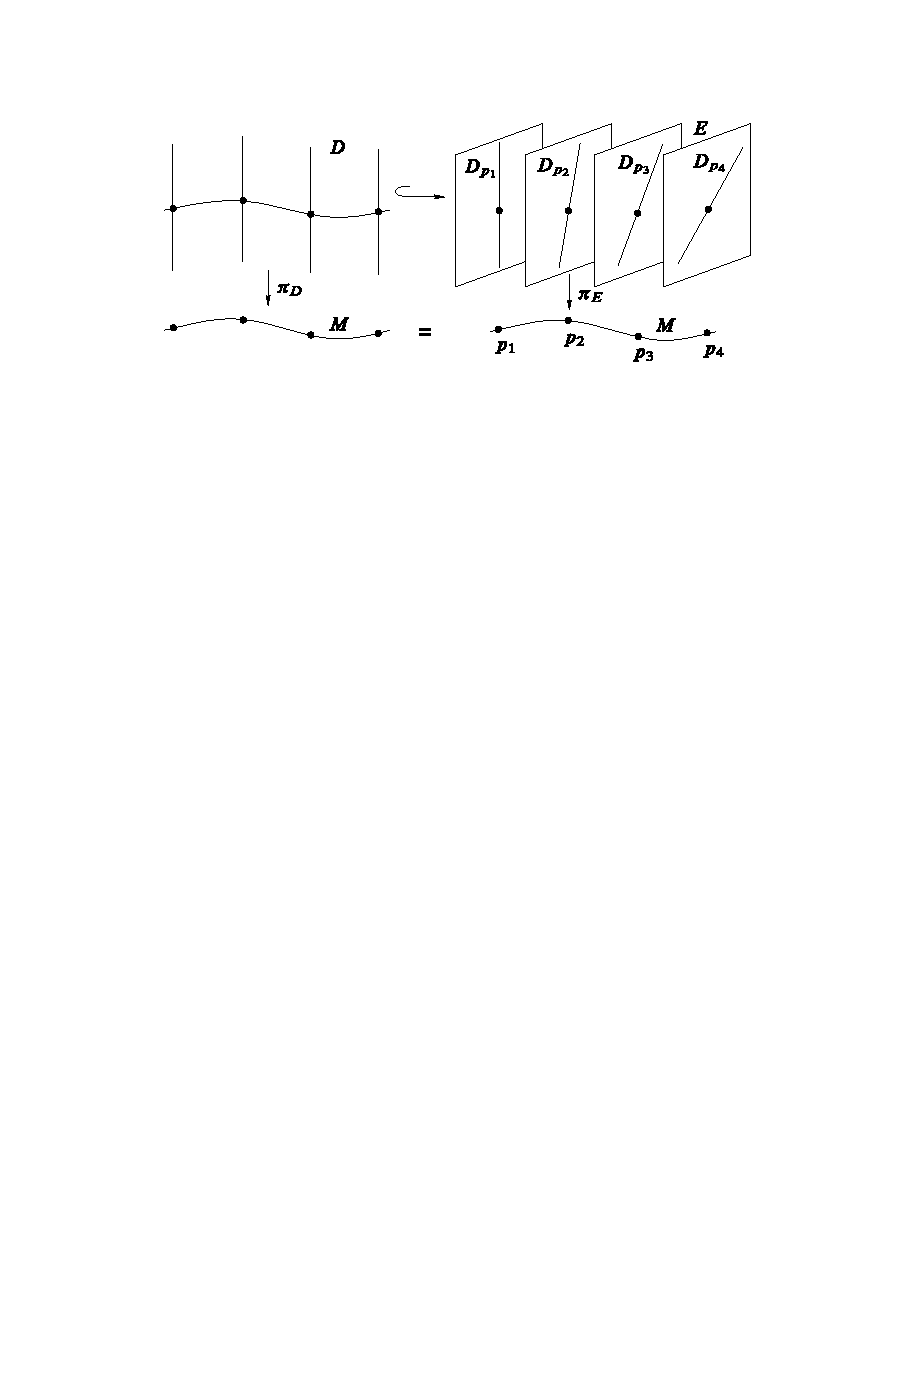
\includegraphics{subbundle}
\caption{A subbundle of a vector bundle.}
\end{figure}
Given a vector bundle $\pi_E:E\to M$, a \textbf{subbundle of $\bm{E}$} is a vector bundle $\pi_D:D\to M$ in which $D$ is a topological subspace of $E$ and $\pi_D$ is the restriction of $\pi_E$ to $D$, such that for each $p\in M$, the subset $D_p=D\cap E_p$ is a linear subspace of $E_p$, and the vector space structure on $D_p$ is the one inherited from $E_p$. Note that the condition that $D$ be a vector bundle over $M$ implies that all of the fibers $D_p$ must be nonempty and have the same dimension. If $E\to M$ is a smooth bundle, then a subbundle of $E$ is called a \textbf{smooth subbundle} if it is a smooth vector bundle and an embedded submanifold with or without boundary in $E$.\par
The following lemma gives a convenient condition for checking that a union of
subspaces $\{D_p\sub E_p:p\in M\}$ is a smooth subbundle.
\begin{lemma}[\textbf{Local Frame Criterion for Subbundles}]\label{vector subbundle crit}
Let $\pi:E\to M$ be a smooth vector bundle, and suppose that for each $p\in M$ we are given an $m$-dimensional linear subspace $D_p\sub E_p$. Then $D=\bigcup_{p\in M}\sub E$ is a smooth subbundle of $E$ if and only if the following condition is satisfied: 
\begin{equation}\label{vector subbundle-1}
\parbox{\dimexpr\linewidth-6em}
{\strut
Each point of $M$ has a neighborhood $U$ on which there exist smooth local sections $\sigma_1,\dots,\sigma_m:U\to E$ with the property that $\sigma_1(q),\dots,\sigma_m(q)$ form a basis for $D_q$ at each $q\in U$.
\strut}
\end{equation}
\end{lemma}
\begin{proof}
If $D$ is a smooth subbundle, then by definition each $p\in M$ has a neighborhood $U$ over which there exists a smooth local trivialization of $D$, and Example~\ref{local frame trivialization} shows that there exists a smooth local frame for $D$ over each such set $U$. Such a local frame is by definition a collection of smooth sections $\tau_1,\dots,\tau_m$ whose images form a basis for $D_p$ at each point $p\in U$. The smooth sections of $E$ that we seek are obtained by composing with the inclusion map $\iota:D\hookrightarrow E$: $\sigma_j=\iota\circ\tau_j$.\par
Conversely, suppose $E\to M$ is a smooth bundle of rank $k$, and $D\sub E$ satisfies $(\ref{vector subbundle-1})$. Each set $D\cap E_p$ is a linear subspace of $E_p$ by hypothesis, so we need to show that $D$ is an embedded submanifold with or without boundary in $E$ and that the restriction of $\pi$ makes it into a smooth vector bundle over $M$. To prove that $D$ is an embedded submanifold with or without boundary, it suffices to show that each $p\in M$ has a neighborhood $U$ such that $D\cap\pi^{-1}(U)$ is an embedded submanifold (possibly with boundary) in $\pi^{-1}(U)\sub E$. Given $p\in M$, let $\sigma_1,\dots,\sigma_m$ be smooth local sections of $E$ satisfying $(\ref{vector subbundle-1})$ on a neighborhood of $p$. By Proposition~\ref{local frame completion}, we can complete these to a smooth local frame $\sigma_1,\dots,\sigma_k$ for $E$ over some neighborhood $U$ of $p$. By Proposition~\ref{local frame iff trivialization}, this local frame is associated with a smooth local trivialization $\varPhi:\pi^{-1}(U)\to U\times\R^k$, defined by
\[\varPhi(s^1\sigma_1(q)+\cdots+s^k\sigma_k(q))=\big(q,(s^1,\dots,s^k)\big).\]
This map $\varPhi$ takes $D\cap\pi^{-1}(U)$ to the subset $\{(q,s)\in U\times\R^k:s^{m+1}=\cdots=s^k=0\}$, which is an embedded submanifold (with boundary if $U$ has a boundary). Moreover, the map $\varPsi:D\cap\pi^{-1}(U)\to U\times\R^m$ defined by
\[\varPsi(s^1\sigma_1(q)+\cdots+s^m\sigma_m(q))=\big(q,(s^1,\dots,s^m)\big),\]
is a smooth local trivialization of $D$, so $D$ is itself a smooth vector bundle.
\end{proof}
\begin{example}[\textbf{Subbundles}]
\mbox{}
\begin{itemize}
\item[(a)] If $M$ is a smooth manifold and $V$ is a nowhere-vanishing smooth vector field on $M$, then the set $D\sub TM$ whose fiber at each $p\in M$ is the linear span of $V_p$ is a smooth $1$-dimensional subbundle of $TM$.
\item[(b)] Suppose $E\sub M$ is any trivial bundle, and let $(E_1,\dots,E_k)$ be a smooth global frame for $E$. If $0\leq m\leq k$, the subset $D\sub E$ defined by $D_p=\mathrm{span}(E_1|_p,\dots,E_m|_p)$ for each $p\in M$ is a smooth subbundle of $E$.
\item[(c)] Suppose $M$ is a smooth manifold with or without boundary and $S\sub M$ is an immersed $k$-submanifold with or without boundary. Then $TS$ is a smooth rank-$k$ subbundle of the ambient tangent bundle $TM|_S$.
\end{itemize}
\end{example}
The next theorem shows how to obtain many more subbundles. Suppose $E\to M$ and $E'\to M$ are vector bundles and $F:E\to E'$ is a bundle homomorphism over $M$. For each $p\in M$, the rank of the linear map $F|_{E_p}$ is called the \textbf{rank of $\bm{F}$ at $\bm{p}$}. We say that $F$ has constant rank if its rank is the same for all $p\in M$.
\begin{theorem}
Let $E$ and $E'$ be smooth vector bundles over a smooth manifold $M$ and let $F:E\to E'$ be a smooth bundle homomorphism over $M$. Define subsets $\ker F\sub E$ and $\im F\sub E'$ by
\[\ker F=\bigcup_{p\in M}\ker(F|_{E_p}),\quad\im F=\bigcup_{p\in M}\im(F|_{E_p}).\]
Then $\ker F$ and $\im F$ are smooth subbundles of $E$ and $E'$, respectively, if and only if $F$ has constant rank.
\end{theorem}
\begin{proof}
One direction is obvious: since the fibers of a bundle have the same dimension everywhere, the constant-rank condition is certainly necessary for $\ker F$ and $\im F$ to be subbundles. To prove sufficiency, suppose $F$ has constant rank $r$, and let $k$ and $k'$ be the ranks of the bundles $E$ and $E'$, respectively. Let $p\in M$ be arbitrary, and choose a smooth local frame $(\sigma_1,\dots,\sigma_k)$ for $E$ over a neighborhood $U$ of $p$. For each $i$, the map $F\circ\sigma_i:U\to E'$ is a smooth local section of $E'$, and these sections span $\im F$. After rearranging the indices if necessary, we can assume that the elements $\{F\circ\sigma_1(p),\dots,F\circ\sigma_r(p)\}$ form a basis for $\im(F|_{E_p})$, and by continuity they remain linearly independent in some neighborhood $U_0$ of $p$. Since $F$ has constant rank, this means that $(F\circ\sigma_1,\dots,F\circ\sigma_r)$ forms a smooth local frame for $\im F$ over $U_0$. Since we can do the same in a neighborhood of each point, the local frame criterion shows that $\im F$ is a smooth subbundle of $E'$.\par
To prove that $\ker F$ is also a smooth subbundle, let $U_0$ and $(\sigma_i)$ be as above, and let $V\sub E|_{U_0}$ be the smooth subbundle spanned by $\sigma_1,\dots,\sigma_r$. The smooth bundle homomorphism $F|_V:V\to(\im F)|_{U_0}$ is bijective, and is thus a smooth bundle isomorphism by Proposition~\ref{vector bundle smooth iso iff bi}. Define a smooth bundle homomorphism $\varPsi:E|_{U_0}\to E_{U_0}$ by
\[\varPsi(v)=v-(F|_V)^{-1}\circ F(v).\]
If $v\in V$, then $F(v)=F|_V(v)$, so $F\circ\varPsi(v)=F(v)-F(v)=0$. On the other hand, if $v\in\ker F$, then $\varPsi(v)=v$ so again $F(\varPsi(v))=F(v)=0$. Since $V$ and $\ker(F)|_{U_0}$ together span $E|_{U_0}$, it follows that $\varPsi$ takes its values in $(\ker F)|_{U_0}$ and since it restricts to the identity on $(\ker F)|_{U_0}$, its image is exactly $(\ker F)|_{U_0}$. Thus $\varPsi$ has constant rank, and by the argument in the preceding paragraph, $(\ker F)|_{U_0}=\im\varPsi$ is a smooth subbundle of $E|_{U_0}$. Since we can do the same thing in a neighborhood of each point, $\ker F$ is a smooth subbundle of $E$.
\end{proof}
The next proposition illustrates another method for constructing interesting subbundles of the tangent bundle over submanifolds of $\R^n$.
\begin{lemma}[\textbf{Orthogonal Complement Bundles}]\label{orthogonal complement bundles}
Let $M$ be an immersed submanifold with or without boundary in $\R^n$, and $D$ be a smooth rank-$k$ subbundle of $T\R^n|_M$. For each $p\in M$, let $D^\bot_p$ denote the orthogonal complement of $D_p$ in $T_p\R^n$ with respect to the Euclidean dot product, and let $D^\bot\sub T\R^n|_M$ be the subset
\[D^\bot=\{(p,v)\in T\R^n:p\in M,v\in D^\bot_p\}\]
Then $D^\bot$ is a smooth rank-$(n-k)$ subbundle of $T\R^n|_M$. For each $p\in M$, there is a smooth orthonormal frame for $D^\bot$ on a neighborhood of $p$.
\end{lemma}
\begin{proof}
Let $p\in M$ be arbitrary, and let $(X_1,\dots,X_k)$ be a smooth local frame for $D$ over some neighborhood $V$ of $p$ in $M$. Because immersed submanifolds are locally 
embedded, by shrinking $V$ if necessary, we may assume that it is a single slice in some coordinate ball or half-ball $U\sub\R^n$. Since $V$ is closed in $U$, 
Proposition~\ref{local frame completion} shows that we can complete $(X_1,\dots,X_k)$ to a smooth local frame $(\widetilde{X}_1,\dots,\widetilde{X}_n)$ for $T\R^n$ 
over $U$, and then Lemma~\ref{Gram-Schmidt frame} yields a smooth orthonormal frame $(E_j)$ over $U$ such that 
\[\mathrm{span}(E_1|_p,\dots,E_k|_p)=\mathrm{span}(X_1|_p,\dots,X_k|_p)=D\]
for each $p\in U$. It follows that $(E_{k+1},\dots,E_n)$ restricts to a smooth orthonormal frame for $D^\bot$ over $V$. Thus $D^\bot$ satisfies the local frame 
criterion, and is therefore a smooth subbundle of $T\R^n|_M$.
\end{proof}
\begin{corollary}[\textbf{The Normal Bundle to a Submanifold of $\R^n$}]
If $M\sub\R^n$ is an immersed $m$-dimensional submanifold with or without boundary, its normal bundle $NM$ is a smooth rank-$(n-m)$ subbundle of $T\R^n|_M$. For each $p\in M$, there exists a smooth orthonormal frame for $NM$ on a neighborhood of $p$.
\end{corollary}
\begin{proof}
Apply Lemma~\ref{orthogonal complement bundles} to the smooth subbundle $TM\sub T\R^n|_M$.
\end{proof}
\subsection{Reduction of structure groups}
Let $E\to M$ be a smooth vector bundle with a trivialization $\{(U_\alpha,\varPhi_{\alpha})\}$. Then by Lemma~\ref{vector bundle cochain prop} the transition functions 
$\{\tau_{\alpha\beta}\}$ satisfy the cocycle condition
\[\tau_{\alpha\beta}\circ\tau_{\beta\gamma}=\tau_{\alpha\gamma}.\]
The cocycle $\{\tau_{\alpha\beta}\}$ clearly depends on the choice of the trivialization $\{\varPhi_\alpha\}$, but we have the following result.
\begin{lemma}\label{vector bundle equivalent transition lem}
Let $\pi:E\to M$ be a smooth vector bundle of rank $k$. If the cocycle $\{\tau'_{\alpha\beta}\}$ comes from another trivialization ${(U_{\alpha},\varPhi'_{\alpha})}$, then there 
exist maps $\sigma_{\alpha}:U_{\alpha}\to \GL_k(\R)$ such that
\[\tau'_{\alpha\beta}(p)=\sigma_\alpha(p)\tau_{\alpha\beta}(p)\sigma_\beta^{-1}(p),\quad p\in U_\alpha\cap U_\beta\]
Two cocycles related in this way are said to be \textbf{equivalent}.
\end{lemma}
\begin{proof}
The two trivializations differ by a nonsingular transformation of $\R^k$ at each point, so there is a map $\sigma_\alpha:U_\alpha\to\GL_k(\R)$ such that
\[\varPhi'_\alpha\circ\varPhi_\alpha^{-1}(p,v)=(p,\sigma_\alpha(p)v)\]
Then
\begin{align*}
\varPhi'_{\alpha}\circ(\varPhi'_{\beta})^{-1}(p,v)&=(\varPhi'_{\alpha}\circ\varPhi_\alpha^{-1})\circ(\varPhi_\alpha\circ\varPhi_\beta^{-1})\circ(\varPhi_{\beta}\circ(\varPhi'_{\beta})^{-1})(p,v)=(p,\sigma_\alpha(p)\tau_{\alpha\beta}(p)\sigma_\beta^{-1}(p)v).
\end{align*}
Therfore we get the desired equality.
\end{proof}
Given a cocycle $\{\tau_{\alpha\beta}\}$ with values in $\GL_k(\R)$ we can construct a vector bundle $E$ having $\{\tau_{\alpha\beta}\}$ as its cocycle as in 
Theorem~\ref{vector bundle construct}. It turns out that the equivalence class of cocycles determines the vector bundle, as the next proposition shows.
\begin{proposition}
Let $\pi:E\to M$ and $\pi':E'\to M$ be two smooth rank-$k$ vector bundles over
a smooth manifold $M$ with or without boundary. Suppose $\{U_\alpha\}_{\alpha\in A}$ is an open cover of $M$ such that both $E$ and $E'$ admit smooth local 
trivializations over each $U_\alpha$. Let $\{\tau_{\alpha\beta}\}$ and $\{\tau'_{\alpha\beta}\}$ denote the transition functions determined by the given local 
trivializations of $E$ and $E'$, respectively. Then $E$ and $E'$ are smoothly isomorphic over $M$ if and only if for each $\alpha\in A$ there exists a smooth map 
$\sigma_\alpha:U_\alpha\to\GL_k(\R)$ such that
\[\tau'_{\alpha\beta}(p)=\sigma_\alpha(p)\tau_{\alpha\beta}(p)\sigma_\beta^{-1}(p),\quad p\in U_\alpha\cap U_\beta.\]
\end{proposition}
\begin{proof}
Assume the given condition for $\{\sigma_\alpha\}$, then the following diagram commutes,
\[\begin{tikzcd}
U_\beta\times\R^k\ar[r,"\sigma_\beta"]\ar[d,swap,"\tau_{\alpha\beta}"]&U_\beta\times\R^k\ar[d,"\tau'_{\alpha\beta}"]\\
U_\alpha\times\R^k\ar[r,"\sigma_\alpha"]&U_\alpha\times\R^k
\end{tikzcd}\]
Thus we can define a map $F:E\to E'$ as following: For $p\in U_\alpha$, let \[\varPhi_\alpha:\pi^{-1}(U_\alpha)\to U\times\R^k\And\varPhi':\pi^{-1}(U_\alpha)\to\R^k\] 
be the local trivializations, respectively. If $(p,v)\in U_\alpha\times\R^k$, we define
\[F(p,v):=(p,\sigma_\alpha(p)v)\]
By our commutative diagram, this definition is in fact coordinate free, thus gives a bundle homomorphism. Since $\sigma_\alpha(p)$ is invertible, $F$ is infact an isomorphism.\par
Conversely, if we are given a bundle homomorphism $F:E\to E'$. Since the restriction of $F$ on each fiber $E_p$ is linear, we can define $\sigma_\alpha$ by
\[\varPhi'_\alpha\circ F\circ\varPhi_\alpha^{-1}(p,v)=(p,\sigma_\alpha(p)v)\]
such that the diagram
\[\begin{tikzcd}
\pi^{-1}(U_\alpha)\ar[d,swap,"\varPhi_\alpha"]\ar[r,"F"]&\pi'^{-1}(U_\alpha)\ar[d,"\varPhi'_\alpha"]\\
U_\alpha\times\R^k\ar[r,dashed,"\sigma_\alpha"]&U_\alpha\times\R^k
\end{tikzcd}\]
commutes. Since $F$ is an isomorphism, each $\sigma_\alpha(p)$ is invertible. Moreover, as for the transition functions, we have the commutative diagram
\[\begin{tikzcd}
U_\beta\times\R^k\ar[r,dashed,"\sigma_\beta"]\ar[dd,bend right=65,swap,"\tau_{\alpha\beta}"]&U_\beta\times\R^k\ar[dd,bend left=65,"\tau'_{\alpha\beta}"]\\
\pi^{-1}(U_\alpha\cap U_\beta)\ar[d,swap,"\varPhi_\alpha"]\ar[u,"\varPhi_\beta"]\ar[r,"F"]&\pi'^{-1}(U_\alpha\cap U_\beta)\ar[d,"\varPhi'_\alpha"]\ar[u,swap,"\varPhi'_\beta"]\\
U_\alpha\times\R^k\ar[r,dashed,"\sigma_\alpha"]&U_\alpha\times\R^k
\end{tikzcd}\]
from which the desired equality can be easily derived:
\[\sigma_\alpha(p)\tau_{\alpha\beta}(p)=\tau'_{\alpha\beta}(p)\sigma_\beta(p)\quad\text{for all }p\in U_\alpha\cap U_\beta.\]
\end{proof}
Given a vector bundle with cocycle $\{\tau_{\alpha\beta}\}$, if it is possible to find an equivalent cocycle with values in a subgroup $H$ of $\GL_k(\R)$, we say that 
the structure group of $E$ may be \textbf{reduced to $\bm{H}$}. A vector bundle is \textbf{orientable} if its structure group may be reduced to $\GL_k^+(\R)$, the 
linear transformations of $\R^k$ with positive determinant. A trivialization $\{(U_\alpha,\varPhi_\alpha)\}_{\alpha\in A}$ on $E$ is said to be \textbf{oriented} if for 
every $\alpha,\beta\in A$, the transition function $\tau_{\alpha\beta}$ has positive determinant. Two oriented trivializations $\{(U_\alpha,\varPhi_\alpha)\}$ 
and $\{(V_\beta,\varPsi_\beta)\}$ are \textbf{equivalent} if for every $p$ in $U_{\alpha}\cap V_{\beta}$, $\varPhi_{\alpha}\circ(\varPsi_\beta)^{-1}$ has positive 
determinant. It is easily checked that this is an equivalence relation and that on a connected manifold $M$ it partitions all the oriented trivializations of the vector 
bundle $E$ into two equivalence classes. Either equivalence class is called an \textbf{orientation on the vector bundle $\bm{E}$}.
\begin{example}[\textbf{The tangent bundle}]
Consider the tangent bundle $TM$ of a smooth manifold $M$. Then the transition functions of $TM$ are the Jacobians of the transition functions of $M$. Therefore $M$ is 
orientable as a manifold if and only if its tangent bundle is orientable as a bundle. (However, the total space of the tangent bundle is always orientable as a manifold, 
see Exercise~\ref{orentaton TM and T^*M}.)
\end{example}
We now show that the structure group of every real vector bundle $E$ may be reduced to the orthogonal group. First, we can endow $E$ with a Riemannian structure-a 
smoothly varying positive definite symmetric bilinear form on each fiber-as follows. Let $\{U_\alpha\}$ be an open cover of $M$ which trivializes $E$. On each $U_\alpha$, 
choose a frame for $E|_{U_\alpha}$ and declare it to be orthonormal. This defines a Riemannian structure on $E|_{U_\alpha}$. Let $g_{\alpha}$ denote this inner product 
on $E|_{U_\alpha}$. Now use a partition of unity $\{\rho_\alpha\}$ to splice them together, i.e., form
\[g=\sum_\alpha\rho_\alpha g_\alpha.\]
This will be an inner product over all of $M$.\par
As trivializations of $E$, we take only those maps $\varPhi_\alpha$ that send orthonormal frames of $E$ (relative to the global metric) to orthonormal frames of $\R^k$-such 
maps exist by the Gram-Schmidt process. Then the transition functions $\tau_{\alpha\beta}$ will preserve orthonormal frames and hence take values in the orthogonal 
group $\O(k)$. If the determinant of $\tau_{\alpha\beta}$ is positive, $\tau_{\alpha\beta}$ will actually be in the special orthogonal group $\SO(k)$. Thus
\begin{proposition}
The structure group of a real vector bundle of rank $k$ can always be reduced to $\O(k)$; it can be reduced to $\SO(k)$ if and only if the vector bundle is orientable.
\end{proposition}
\subsection{Operations on vector bundles}
\subsubsection{Quotient bundle}
Suppose $D$ is a smooth subbundle of a smooth vector bundle $\pi:E\to M$. At each point $p$ in $M$, the fiber $D_p$ is a vector subspace of $E_p$ and so the quotient 
space $Q_p:=E_p/D_p$ is defined. Let
\[Q=\coprod_{p\in M}Q_p=\coprod_{p\in M}(E_p/D_p),\]
and give $Q$ the quotient topology as a quotient space of $E$. Let $\rho:E\to Q$ be the quotient map. The projection $\pi:E\to M$ then induces a map $\pi_Q:Q\to M$ as 
in the commutative diagram
\[\begin{tikzcd}
D\ar[r,hook]&E\ar[d,swap,"\pi"]\ar[r]&Q\ar[ld,"\pi_Q"]\\
&M&
\end{tikzcd}\]
Since $F$ is locally trivial, every point $p$ in $M$ has a coordinate neighborhood over which one can find a smooth frame $(\sigma_1,\dots,\sigma_k)$ for $D$. By 
Lemma~\ref{vector bundle local frame completion}, $(\sigma_1,\dots,\sigma_k)$ can be extended to a smooth frame $(\sigma_1,\dots,\sigma_k,\sigma_{k+1},\dots,\sigma_r)$ 
for $E$ over a possibly smaller neighborhood $W$ of $p$. A point $v$ of $E|_W$ is uniquely a linear combination $v=v^i\sigma_i$ where $v^i$ are smooth. Let 
$\widebar{\sigma}_{k+1},\dots,\widebar{\sigma}_r:W\to Q$ be the sections $\sigma_{k+1},\dots,\sigma_r$ followed by the projection $E\to Q$. Then 
$(\widebar{\sigma}_{k+1},\dots,\widebar{\sigma}_r)$ is a continuous frame for $Q$ over $W$, and by Proposition~\ref{local frame iff trivialization} we get a homeomorphism
\[\varPsi_W(q,(\widebar{v}^1,\dots,\widebar{v}^{r-k}))=\widebar{v}^i\widebar{\sigma}_i(q).\]
Moreover, it is clear that the collection $\{\varPsi_W\}$ satisfies the conditions of Lemma~\ref{vector bundle chart lemma}. Therefore one can give $Q$ a manifold 
structure as well as a smooth vector bundle structure over $M$. With this vector bundle structure, $\pi_Q:Q\to M$ is called the 
\textbf{quotient bundle of $\bm{E}$ by $\bm{D}$}.
\subsubsection{Other operations on vector bundles}
Let $\mathcal{V}$ be the category whose objects are finite-dimensional real vector spaces and whose morphisms are isomorphisms of vector spaces. In this category, if 
two vector spaces have different dimensions, then the set of morphisms between them is the empty set. Denote by $\mathcal{V}\times\mathcal{V}$ the category whose 
objects are pairs of finite-dimensional vector spaces and whose morphisms are pairs of isomorphisms of vector spaces.\par
If $V$ and $V'$ are finite-dimensional vector spaces of the same dimension $n$, let $Iso(V,V')$ be the set of all isomorphisms from $V$ to $V'$. With respect to fixed 
bases for $V$ and $V'$, elements of $\Iso(V,V')$ are represented by nonsingular $n\times n$ matrices. Hence, $\Iso(V,V')$ is bijective with $\GL_n(\R)$, and therefore 
has the structure of a manifold. A functor $\mathscr{D}:\mathcal{V}\to\mathcal{V}$ is said to be \textbf{smooth} if for all finite-dimensional vector spaces $V$ and $V'$ the map
\[\mathscr{D}:\Iso(V,V')\to\Iso(\mathscr{D}(V),\mathscr{D}(V')),\quad f\mapsto\mathscr{D}(f)\]
is smooth.\par
Similarly, a functor $\mathscr{T}:\mathcal{V}\times\mathcal{V}\to\mathcal{V}$ is said to be smooth if for all finite-dimensional vector spaces
$V$, $V'$, $W$, $W'$ with $\dim V=\dim V'$ and $\dim W=\dim W'$, the map
\[\mathscr{T}:\Iso(V,V')\times\Iso(W,W')\to\Iso(\mathscr{T}(V,W),\Iso(V',W')),\quad (f,g)\mapsto\mathscr{T}(f,g)\]
is smooth.
\begin{example}
Let $\mathscr{T}(V,W)=V\oplus W$. This is a smooth functor because if $f:V\to V'$ and $g:W\to W'$ are isomorphisms represented by matrices $M_f$ and $M_g$ relative to 
some bases, then $f\oplus g:V\oplus W\to V'\oplus W'$ is represented by the matrix
\[\begin{pmatrix}
M_f&0\\
0&M_g
\end{pmatrix}\]
relative to the same bases.
\end{example}
\begin{example}
Similarly, the functor $\mathscr{T}(V,W)=V\otimes W$ is also a smooth functor since if $f:V\to V'$ and $g:W\to W'$ are isomorphisms represented by matrices $M_f$ and $M_g$ 
relative to some bases, then $f\otimes g:V\otimes W\to V'\otimes W'$ is represented by the matrix $M_f\otimes M_g$.
\end{example}
Now we have the following general result for a smooth functor $\mathscr{T}:\mathcal{V}\times\mathcal{V}\to\mathcal{V}$.
\begin{proposition}
If $\mathscr{T}:\mathcal{V}\to\mathcal{V}$ is a smooth covariant functor, then for any smooth vector bundles $E$ over a manifold $M$, there is a smooth 
vector bundle $\mathscr{T}(E)$ over $M$ whose fiber at $p\in M$ is $\mathscr{T}(E_p)$.\par
Similarly, if $\mathscr{T}:\mathcal{V}\times\mathcal{V}\to\mathcal{V}$ is a smooth covariant functor, then for any two smooth vector bundles $E$ and $E'$ over a 
manifold $M$, there is a smooth vector bundle $\mathscr{T}(E,F)$ over $M$ whose fiber at $p\in M$ is $\mathscr{T}(E_p,E'_p)$.
\end{proposition}
\begin{proof}
We only prove the second claim, since the first can be proved in the same manner.\par
Let $\{U_\alpha\}_{\alpha\in A}$ and $\{V_\beta\}_{\beta\in B}$ be trivializing open covers for $E$ and $E'$, respectively, then $\{U_\alpha\cap V_\beta\}_{\alpha\in A,\beta\in B}$ 
is an open cover of $M$ that simultaneously trivializes both $E$ and $E'$. Therefore for each $p\in U_\alpha\cap V_{\beta}$ we have isomorphisms
\[\varPsi_{\alpha,p}:E_p\to\{p\}\times\R^k,\quad \varPhi_{\beta,p}:E'_p\to\{p\}\times\R^{k'}\]
and therefore an isomorphism
\[\mathscr{T}(\varPsi_{\alpha,p},\varPhi_{\beta,p}):\mathscr{T}(E_p,E'_p)\to\{p\}\times\mathscr{T}(\R^{k},\R^{k'}).\]
We then get a bijection
\[\mathscr{T}(\varPsi_\alpha,\varPhi_\beta):\coprod_{p\in U_{\alpha}\cap V_{\beta}}\mathscr{T}(E_p,E'_p)\to (U_\alpha\cap U_{\beta})\times\mathscr{T}(\R^{k},\R^{k'}).\]
Moreover, if $(\alpha,\beta),(\alpha',\beta')\in A\times B$, then on the overlap $(U_\alpha\cap V_\beta)\cap(U_{\alpha'}\cap V_{\beta'})$ the map $\mathscr{T}(\varPsi_\alpha,\varPhi_\beta)\circ\mathscr{T}(\varPsi_\alpha,\varPhi_\beta)^{-1}$ 
has the form
\[(p,v)\mapsto(p,\tau_{(\alpha,\beta),(\alpha',\beta')}(p)v)\]
where $\tau_{(\alpha,\beta),(\alpha',\beta')}:(U_\alpha\cap V_\beta)\cap(U_{\alpha'}\cap V_{\beta'})\to\GL(\mathscr{T}(\R^k,\R^{k'}))$ is given by
\[\tau_{(\alpha,\beta),(\alpha',\beta')}(p)=\mathscr{T}(\tau_{\alpha,\alpha'}(p),\tau_{\beta,\beta'}(p)).\]
Therefore we see the conditions in Lemma~\ref{vector bundle chart lemma} is satisfied, so there is a smooth vector bundle $\mathscr{T}(E,F)$ over $M$ whose fiber at 
$p\in M$ is $\mathscr{T}(E_p,E'_p)$. 
\end{proof}
If a functor is contravariant, it must be turned into a covariant functor first to apply this construction. For example, consider the dual functor applied to a vector 
bundle $E\to M$. Because of its contravariance, it associates to a trivialization
\[\varPsi_p:E_p\to\{p\}\times\R^k\]
the map
\[\varPsi^*_p:\{p\}\times(\R^k)^*\to E_p^*.\]
We need to take the inverse of $\varPsi_p^*$ to get a trivialization that goes in the right direction,
\[(\varPsi^*_p)^{-1}:E_p^*\to\{p\}\times(\R^k)^*.\]
To construct the dual bundle, the functor $\mathscr{T}:V\to V$ associates to every finite-dimensional vector space $V$ its dual space $V^*$, and to every isomorphism 
$f:V\to W$ the isomorphism $(f^*)^{-1}:V^*\to W^*$.\par
In the category $\mathcal{V}$ the morphisms are all isomorphisms precisely so that one can reverse the direction of a map and make a contravariant functor covariant. 
In this way, starting from smooth vector bundles $E$ and $E'$ over $M$, one can construct smooth vector bundles $E\oplus E'$, $E\otimes E'$, $\bigwedge^kE$, $E^*$, and 
$\Hom(E,E')=E^*\otimes E'$ over $M$.
\subsubsection{The pullback bundle}
If $\pi:E\to M$ is a smooth vector bundle over a manifold $M$ and $f:N\to M$ is a smooth map, then there is a smooth vector bundle $f^*E$ over $N$, called the \textbf{pullback 
of $\bm{E}$ by $\bm{f}$}, with the property that every bundle map covering $F$ factors through the pullback bundle $f^*E$.\par
The total space of the pullback bundle of $E$ by $F$ is defined to be the set
\[f^*E=\{(q,e)\in N\times E:f(q)=\pi(e)\}.\]
endowed with the subspace topology. The projections to the two factors fit into a commutative diagram
\[\begin{tikzcd}
f^*\ar[r]\ar[d]&E\ar[d,"\pi"]&\\
N\ar[r,"f"]&M
\end{tikzcd}\]
We will show that $\eta:f^*E\to N$ is a vector bundle. First, we show that the pullback of a product bundle is a product bundle.
\begin{proposition}\label{vector bundle pullback}
If $f:N\to M$ is a smooth map of manifolds and $\pi:E=M\times V\to M$ is a product bundle, then the projection $f^*E\to N$ is isomorphic to the product bundle 
$N\times V\to N$.
\end{proposition}
\begin{proof}
As a set,
\[f^*E=\{(q,(p,v))\in N\times(M\times V):f(q)=\pi(p,v)=p\}=\{(q,(f(q),v))\in N\times(M\times V)\}.\]
Therefore the map
\[T:f^*E\to N\times V,\quad (q,(f(q),v))\mapsto(q,v)\]
with inverse $(q,v)\mapsto(q,(f(q),v))$ is a fiber-preserving homeomorphism. It gives $f^*E\to N$ the structure of a smooth vector bundle over $N$.
\end{proof}
\begin{corollary}
Let $\pi:E\to M$ be a smooth vector bundle with fiber $V$ and $f:N\to M$ a smooth map. The projection $f^*E\to N$ can be given the structure of a smooth vector bundle 
with fiber $V$.
\end{corollary}
\begin{proof}
Since $E$ is locally a product $U\times V\to U$, by Proposition~\ref{vector bundle pullback}, the pullback $f^*E$ is locally the product $f^{-1}(U)\times V\to f^{-1}(U)$.
\end{proof}
Now we determine the transition functions of the pullback bundle $f^*E$ from that of $E$. First we need a lemma.
\begin{lemma}
Suppose $\pi:E\to M$ is a smooth vector bundle with fiber $V$ and $f:N\to M$ is a smooth map. Let $U$ be an open subset of $M$. Then
\[(f^*E)|_{f^{-1}(U)}=f^*(E|_U).\]
\end{lemma}
\begin{proof}
By definition we have
\begin{align*}
(f^*E)|_{f^{-1}(U)}&=\{(q,e)\in N\times E:q\in f^{-1}(U),f(q)=\pi(e)\}\\
&=\{(q,e)\in f^{-1}(U)\times E:f(q)=\pi(e)\}=f^*(E|_U).
\end{align*}
Therefore the claim follows.
\end{proof}
\begin{proposition}
Suppose $\pi:E\to M$ is a smooth vector bundle with fiber $V$ and trivializing open cover $\{U_\alpha\}$ and $f:N\to M$ is a smooth map. If 
$\rho_{\alpha\beta}:U_\alpha\cap U_\beta\to\GL(V)$ is the transition function for $E$ over $U_\alpha\cap U_\beta$, then $f^*\rho_{\alpha\beta}$ is the transition 
function for $f^*E$ over $F^{-1}(U_\alpha\cap U_\beta)$.
\end{proposition}
\begin{proof}
Suppose $\varPsi_\alpha:U_\alpha\times\R^k\to\pi^{-1}(U_\alpha)$ is the trivialization for $E$ over $U_\alpha$, then the trivalization of $F^{-1}(U)$ is 
given by
\[\widetilde{\varPsi}_\alpha:f^{-1}(U)\times V\to f^*(E|_{f^{-1}(U_\alpha)}),\quad (q,v)\mapsto(q,\varPsi_\alpha(f(q),v)).\]
Therefore the transition function $\widetilde{\varPsi}_\alpha\circ\widetilde{\varPsi}_\beta^{-1}$ is given by
\[\widetilde{\varPsi}_\alpha\circ\widetilde{\varPsi}_\beta^{-1}(q,v)=(q,\rho_{\alpha\beta}(f(q))v).\]
This gives the claim.
\end{proof}
Finnaly, we can now prove the desired pullback property of the pullback bundle.
\begin{theorem}\label{vector bundle pullback universal prop}
Suppose $\pi':E'\to N$ and $\pi:E\to M$ are vector bundles and $F:E'\to E$ is a bundle map that covers $f:N\to M$, i.e., the diagram
\begin{equation}\label{vector bundle pullback universal-1}
\begin{tikzcd}
E'\ar[r,"F"]\ar[d,swap,"\pi'"]&E\ar[d,"\pi"]\\
N\ar[r,"f"]&M
\end{tikzcd}
\end{equation}
Then there is a unique bundle map 
$\widetilde{F}:E'\to f^*E$ over $N$ that makes the following diagram commute:
\begin{equation}\label{vector bundle pullback universal-2}
\begin{tikzcd}
E'\ar[rrd,bend left=20pt,"F"]\ar[rdd,bend right=20pt,swap,"\pi'"]\ar[rd,dashed,"\widetilde{F}"]&&\\
&f^*E\ar[d]\ar[r]&E\ar[d,"\pi"]\\
&N\ar[r,"f"]&M
\end{tikzcd}
\end{equation}
\end{theorem}
\begin{proof}
The commutativity of the diagram $(\ref{vector bundle pullback universal-1})$ forces $\widetilde{F}(e')=(\pi'(e'),F(e'))$, so the map $\widetilde{F}$ as defined above 
indeed exists and is unique. It is $\R$-linear on each fiber because $F$ is. It is smooth because $\pi'$ and $F$ are assumed to be smooth.
\end{proof}
\begin{example}[\textbf{The differential of a map}]
If $f:N\to M$ is a smooth map of manifolds, its differentials $df_p:T_pN\to T_{F(p)}M$ at all points $p\in N$ piece together to give a bundle map $df:TN\to TM$ of 
tangent bundles. By Theorem~\ref{vector bundle pullback universal prop}, the bundle map $df$ induces a unique bundle map $\widetilde{df}:TN\to f^*TM$ over $N$ that 
makes the diagram
\[\begin{tikzcd}
TN\ar[rrd,bend left=20pt,"df"]\ar[rdd,bend right=20pt,swap,"\pi'"]\ar[rd,dashed,"\widetilde{df}"]&&\\
&f^*TM\ar[d]\ar[r]&TM\ar[d,"\pi"]\\
&N\ar[r,"f"]&M
\end{tikzcd}\]
commutative. The map $\widetilde{df}$ is given by
\[X_p\in T_pN\mapsto(p,df_p(X_p))\]
Conversely, $df$ can be obtained from $\widetilde{df}\circ\pi_{TM}$. In this way the bundle map $df$ over two base manifolds is converted to a bundle map $\widetilde{df}$ 
over the single manifold $N$.
\end{example}
\begin{example}[\textbf{Vector fields along a curve}]
If $\gamma:I\to M$ is a smooth map from an open interval $I\sub\R$ into a manifold $M$, then the pullback $\gamma^*TM$ of the tangent bundle $TM$ is a vector bundle 
over $I$. A section of the pullback bundle $\gamma^*TM$ assigns to each $t\in I$ an element of the fiber $(\gamma^*TM)_t\cong T_{\gamma(t)}M$, i.e., a tangent vector 
to $M$ at $\gamma(t)$. In other words, a section of $\gamma^*TM$ is precisely a vector field along the curve $\gamma(t)$ in $M$. Therefore a vector field along a curve 
$\gamma$ in $M$ is smooth if and only if the corresponding section of $\gamma^*TM$ is smooth.
\end{example}
Let $\mathsf{Vect}_k(M)$ be the isomorphism classes of rank $k$ real vector bundles over $M$. It is a pointed set with base point the isomorphism class of the trivial 
bundle over M. If $f:M\to N$ is a map between two manifolds, let $\mathsf{Vect}_k(f)=f^*$ be the pullback map on bundles. In this way, for each integer $k$, $\mathsf{Vect}_k$ 
becomes a contravariant functor from the category of manifolds and smooth maps to the category of pointed sets and base point preserving maps.\par
As an application of the constructions above, we prove an important fact about the pullback bundle.
\begin{proposition}[\textbf{Homotopy Property of Vector Bundles}]
Assume $N$ to be a compact manifold. If $f_0$ and $f_1$ are homotopic maps from $N$ to a manifold $X$ and $E$ is a vector bundle on $M$, then $f_0^*E$ is isomorphic to 
$f_1^*E$, i.e., homotopic maps induce isomorphic bundles.
\end{proposition}
\begin{proof}
Let $f:N\times I\to M$ be a homotopy between $f_0$ and $f_1$ and let $\pi:N\times I\to N$ be the projection. Suppose for some $t_0$ in $I$, $f_{t_0}^*E$ is isomorphic
to some vector bundle $F$ on $N$. We will show that for all $t$ near $t_0$, $f_{t}^*E\cong F$. By the compactness and connectedness of the unit interval $I$ it will 
then follow that $f_t^*E\cong F$ for all $t$ in $I$.\par
Over $N\times I$ there are two pullback bundles, $f^*E$ and $\pi^*F$. Since $f_{t_0}^*E\cong F$, the bundle $\Iso(f^*E,\pi^*F)$ has a section over $N\times\{t_0\}$, 
which a priori is also a section of $\Hom(f^*E,\pi^*F)$. Since $N$ is compact, $N\times\{t_0\}$ may be covered with a finite number of trivializing open sets for 
$\Hom(f^*E,\pi^*F)$. As the fibers of $\Hom(f^*E,\pi^*F)$ are Euclidean spaces, the section over $N\times\{t_0\}$ may be extended to a section of $\Hom(f^*E,\pi^*F)$ 
over the union of these open sets. Now any linear map near an isomorphism remains an isomorphism, thus we can extend the given section of $\Iso(f^*E,\pi^*F)$ to a 
strip containing $N\times\{t_0\}$ (by the tube lemma). This proves that $f_t^*E\cong F$ for $t$ near $t_0$. We now cover $N\times I$ with a finite number of such 
strips. Hence $f_0^*E\cong f_1^*E$.
\end{proof}
But the same argument can be refined to give the theorem for $N$ a paracompact space. Since every manifold is paracompact, this result actually holds for all manifolds, 
compact or not.
\begin{corollary}
A vector bundle over a contractible manifold is trivial.
\end{corollary}
\begin{proof}
Let $E$ be a vector bundle over $M$ and let $f:M\to\{\ast\}$ be an homotopy equivalence between $M$ and $\{\ast\}$. Then we can see that $f^*$ is an isomorphism on 
vector bundles. Since every vector bundle on $\{\ast\}$ is trivial, so is that on $M$.
\end{proof}
So for a contractible manifold $M$, $\mathsf{Vect}_k(M)$ is a single point.
\subsection{Fiber bundles}
Let $M$ and $F$ be topological spaces. A \textbf{fiber bundle over $M$ with model fiber $\bm{F}$} is a topological space $E$ together with a surjective continuous map $\pi:E\to M$ with the property that for each $x\in M$, there exist a neighborhood $U$ of $x$ in $M$ and a homeomorphism $\varPhi:\pi^{-1}(U)\to U\times F$, called a \textbf{local trivialization of $\bm{E}$ over $\bm{U}$}, such that the following diagram commutes:
\[\begin{tikzcd}
\pi^{-1}(U)\ar[rr,"\varPhi"]\ar[rd,swap,"\pi"]&&U\times F\ar[ld,"\pi_U"]\\
&U&
\end{tikzcd}\]
The space $E$ is called the \textbf{total space of the bundle}, $M$ is its \textbf{base}, and $\pi$ is its \textbf{projection}. If $E,M$ and $F$ are 
smooth manifolds with or without boundary, $\pi$ is a smooth map, and the local trivializations can be chosen to be diffeomorphisms, then it is called 
a \textbf{smooth fiber bundle}. If $\pi:E\to M$ be a smooth fiber bundle with fiber $F$ over $M$, a \textbf{bundle chart} is a pair $(U,\varPhi)$ where 
$U$ is open in $M$ and $\varPhi:\pi^{-1}(U)\to U\times F$ is a smooth local trivialization. A \textbf{bundle atlas} on $E$ is a collection of bundle 
charts whose domains cover $M$.\par
A \textbf{trivial fiber bundle} is one that admits a local trivialization over the entire base space (a \textbf{global trivialization}). It is said to be \textbf{smoothly trivial} if it is a smooth bundle and the global trivialization is a diffeomorphism.
\begin{example}[\textbf{Fiber Bundles}]\label{fiber bundle eg}
\mbox{}
\begin{itemize}
\item[(a)]Every product space $M\times F$ is a fiber bundle with projection $\pi_1:M\times F\to M$ called a \textbf{product fiber bundle}. It has a global trivialization given by the identity map $M\times F\to M\times F$, so every product bundle is trivial.
\item[(b)]Every rank-$k$ vector bundle is a fiber bundle with model fiber $\R^k$.
\item[(c)]If $E\to S^1$ is the M\"obius bundle, then the image of $\R\times[-1,1]$ under the quotient map $q:\R^2\to E$ is a fiber bundle over $S^1$ with model fiber $[-1,1]$. It is not a trivial bundle.
\item[(d)]Every covering map $\pi:E\to M$ is a fiber bundle whose model fiber is discrete. To construct local trivializations, let $S$ be a discrete space 
with the same cardinality as the fibers of $\pi$. For each evenly covered open subset $U\sub M$, define a map $\varPhi:\pi^{-1}(U)\to U\times S$ by choosing 
a bijection between the set of components of $\pi^{-1}$ and $S$, and letting $\varPhi(x)=(\pi(x),c(x))$, where $c(x)$ is the element of $S$ corresponding to 
the component containing $x$.
\end{itemize}
\end{example}
\begin{proposition}
Let $\pi:E\to M$ be a smooth fiber bundle with fiber $F$ over $M$. Then $\pi$ is a submersion. Furthermore, for each $p\in M$ the 
fiber $E_p$ is a properly embedded submanifold diffeomorphic to $F$.
\end{proposition}
\begin{proof}
Let $\varPhi:\pi^{-1}(U)\to U\times F$ be a smooth local trivialization over an open set $U$ in $M$. Then $\pi|_{\pi^{-1}(U)}=\pi_U\circ\varPhi$. Since $\pi_U$ and $\varPhi$ are both submersions, it follows 
that $\pi|_{\pi^{-1}(U)}$ is also a submersion. Since $U$ is arbitrary, we see $\pi$ is a submersion. Then by Corollary~\ref{subm level set}, each fiber of it is naturally a properly embedded submanifold of $E$. For each $p\in U$, $\varPhi$ maps $E_p$ diffeomorphically onto the embedded submanifold $\{p\}\times F$ of $U\times F$, and $\pi_F$ is a diffeomorphism from this onto $F$.
\end{proof}
Due to this proposition, the bundle $E$ over $M$ with fiber $F$ is occasionally denoted, by abuse of notation, by the symbol $F\to E\stackrel{\pi}{\to}M$.
\begin{lemma}\label{fiber bundle trivialization overlap}
Let $\pi:E\to M$ be a smooth fiber bundle with fiber $F$ over $M$. Suppose $\varPhi:\pi^{-1}(U)\to U\times F$ and $\varPsi:\pi^{-1}(V)\to V\times F$ are two smooth 
local trivializations of $E$ with $U\cap V=\emp$. There exists a smooth map $\tau:U\cap V\to\Diff(F)$ such that the composition $\varPhi\circ\varPsi^{-1}:(U\cap V)\times\R^k\to(U\cap V)\times F$ has the 
form
\[\varPhi\circ\varPsi^{-1}(p,v)=(p,\tau(p)(v)).\]
The map $\tau:U\cap V\to\Diff(F)$ is called the \textbf{transition function} between $\varPhi$ and $\varPsi$.
\end{lemma}
In the smooth case, the group $\Diff(F)$ is to large to deal with, and it is often convenient to require the transition functions to take values in a Lie group $G$. More precisely, we make the following definition.
\begin{definition}
A Lie group $G$ is said to be a \textbf{Lie transformation group} on a manifold $F$ if there is given a smooth left action of $G$ on $F$. Let $G$ be a Lie group acting 
on $F$ on the left. Bundle charts $(U,\varPhi)$ and $(V,\varPsi)$ in $M$ will be said to be \textbf{$\bm{G}$-compatible} if $U\cap V=\emp$, or if $U\cap V\neq\emp$ 
and there exists a smooth map $\tau:U\cap V\to G$ such that 
\[\varPhi\circ\varPsi^{-1}(p,v)=(p,\tau_p\cdot v)\]
for all $(p,v)\in(U\cap V)\times F$. That is, the traisition function is given by an element of $G$.
\end{definition}
\begin{definition}
Let $G$ be a Lie group. A smooth fiber bundle $F\to E\stackrel{\pi}{\to}M$ is called a \textbf{smooth bundle with structure group $\bm{G}$} if $G$ is a Lie transformation group on $F$, and there is given 
a bundle atlas $\mathcal{A}$ on $E$ such that any two bundle charts in $\mathcal{A}$ are $G$-compatible. A smooth fiber bundle chart is \textbf{admissible} as a bundle chart on the bundle $E$ with structure group $G$ if it is $G$-compatible with every element of the given $G$-bundle atlas.
\end{definition}
Therefore, vector bundles can be viewed as $\GL_k(\R)$-bundles with fiber $\R^k$. The following lemma can be viewed as a generalization of Lemma~\ref{vector bundle chart lemma}.
\begin{lemma}[\textbf{Fiber Bundle Chart Lemma}]\label{fiber bundle chart lemma}
Let $M$ and $F$ be a smooth manifolds with or without boundary, and suppose that for each $p\in M$ we are given a manifold $E_p$ diffeomorphic to $F$. Let $E=\coprod_{p\in M}E_p$ and let 
$\pi:E\to M$ be the map that takes each element of $E_p$ to the point $p$. Suppose furthermore that we are given the following 
data:
\begin{itemize}
\item[$(\rmnum{1})$] An open cover $\{U_\alpha\}_{\alpha\in A}$ of $M$.
\item[$(\rmnum{2})$] For each $\alpha\in A$, a bijective map $\varPhi_\alpha:\pi^{-1}(U_\alpha)\to U_\alpha\times F$ whose restriction to each $E_p$ is a diffeomorphism from $E_p$ to $\{p\}\times F$.
\item[$(\rmnum{3})$] For each $\alpha,\beta\in A$ with $U_\alpha\cap U_\beta\neq\emp$, a smooth map $\tau_{\alpha\beta}:U_\alpha\cap U_\beta\to G$ such that the map $\varPhi_\alpha\circ\varPhi_\beta^{-1}$ from $(U_\alpha\cap U_\beta)\times F$ to itself has the form
\begin{align}\label{fiber bundle transition function-1}
\varPhi_\alpha\circ\varPhi_\beta^{-1}(p,v)=(p,\tau_{\alpha\beta}(p)\cdot(v))
\end{align}
where $G$ is a Lie group acting on $F$.
\end{itemize}
Then $E$ has a unique topology and smooth structure making it into a smooth manifold with or without boundary and a smooth fiber bundle over $M$ with fiber $F$ and structure group $G$, with $\pi$
as projection and $\{(U_\alpha,\varPhi_\alpha)\}$ as smooth local trivializations.
\end{lemma}
\begin{theorem}[\textbf{Fiber bundle construction theorem}]\label{fiber bundle construct Lie group}
Let $M$ and $F$ be smooth manifolds with or without boundary, and let $\{U_\alpha\}_{\alpha\in A}$ be an open cover of $M$. Suppose that there is a Lie group $G$ acting on $F$ and for each $\alpha,\beta\in A$ we are 
given a smooth map $\tau_{\alpha\beta}:U_{\alpha}\cap U_{\beta}\to G$ such that $(\ref{fiber bundle transition function-1})$ is satisfied for all $\alpha,\beta,\gamma\in A$. Then 
there is a smooth fiber bundle $\pi:E\to M$ with fiber $F$, sturcture group $G$ and smooth local trivializations $\varPhi_\alpha:\pi^{-1}(U_\alpha)\to U_\alpha\times F$ 
whose transition functions are the given maps $\tau_{\alpha\beta}$.
\end{theorem}
\begin{example}[\textbf{The universal Une bundle over a projective space}]
Let $n>0$, consider the real projective space $\RP^n$. Let $\pi:\R^{n+1}\setminus\{0\}\to\RP^n$ be the projection map. 
For each $i=0,\dots,n$, let $\widetilde{U}_i\sub\R^{n+1}\setminus\{0\}$ be the set where $x_i\neq 0$, and let 
$U_i=\pi(\widetilde{U}_i)\sub\RP^n$. Since $\widetilde{U}_i$ is a saturated open subset, $U_i$ is open and $\pi|_{\widetilde{U}_i}$ is a 
quotient map. Define a map $\varphi$ by
\[\varphi_i[x^0,\dots,x^{n}]=\Big(\frac{x^0}{x^i},\dots,\frac{x^{i-1}}{x^i},\frac{x^{i+1}}{x^i},\dots,\frac{x^{n}}{x^i}\Big)\]
Now we make $\R^{n+1}\setminus\{0\}$ into the total space of a fiber bundle over $\RP^n$ with standard fiber $\R\setminus\{0\}$. 
Define $\varPhi_1:\pi^{-1}(U_i)\to U_i\times(\R\setminus\{0\})$ by 
\[\varPhi_i(x^0,\dots,x^n)=([x^0,\dots,x^n],x^i).\]
The maps $(U_i,\varPhi_i)$ will be bundle charts once it is checked that they generate a smooth structure on $\R^{n+1}\setminus\{0\}$.\par
Let $i\neq j$, for all $(p,v)\in\pi^{-1}(U_i\cap U_j)\times(\R\setminus\{0\})$, we have 
\[\varPhi_i\circ\varPhi_j^{-1}([x^0,\dots,x^n],v)=\varPhi_i(\frac{v}{x^j}\cdot(x^0,\dots,x^n))=([x^0,\dots,x^n],\frac{x^i}{x^j}\cdot v).\]
Thus the maps $\varPhi_i$ determine a smooth fiber bundle $\R^{n+1}\setminus\{0\}\to\RP^n$ with fiber $\R\setminus\{0\}$ and sturcture group $\GL_1(\R)$ by Lemma~\ref{fiber bundle chart lemma}.\par
The bundle $\R^{n+1}\setminus\{0\}$ over $\RP^n$ is canonically a subbundle of a
bundle $E\to\RP^n$ with fiber $\R$. For each $p\in\RP^n$, define $E_p=\pi^{-1}(p)\cup\{(p,0)\}$. All that has really been added to $\pi^{-1}(p)$ 
the point $0$ in $\R$; calling the new point $(p,0)$ instead of just $0$ is a technical 
device to guarantee that distinct fibers in the new bundle have distinct zero points. Set $E$ equal to the union over all $p\in\RP^n$ of $E_p$, and extend the maps by $\pi(p,0)=p$ 
and $\varPhi_i(p,0)=(p,0)\in U_i\times\R$. Then by Lemma~\ref{fiber bundle chart lemma} again, $E\to\RP^n$ is a smooth fiber bundle with fiber $\R$.\par
The constructions above can also be done on $\CP^n$. The fiber bundle $\R\to\R^{n+1}\stackrel{\pi}{\to}\RP^n$ ($\C\to\C^{n+1}\stackrel{\pi}{\to}\CP^n$) is called the \textbf{universal line bundle} over $\RP^n$ 
($\CP^n$).
\end{example}
\begin{example}[\textbf{Milnor's exotic spheres}]
Let $N$ be the north pole $(0,\dots,0,1)$ in $S^n\sub\R^{n+1}$ and $S$ the south pole $(0,\dots,0,-1)$. Set $U:=S^n-\{N\}$ and $V:=S^n-\{S\}$. The stereographic 
projection of $S^n$ onto the equatorial plane from $N$ is the map
\[\varphi:U\to\R^n,\quad (x^1,\dots,x^{n+1})\mapsto\frac{(x^1,\dots,x^n)}{1-x^{n+1}}.\]
The stereographic projection of $S^n$ from $S$ is the map
\[\psi:V\to\R^n,\quad (x^1,\dots,x^{n+1})\mapsto\frac{(x^1,\dots,x^n)}{1+x^{n+1}}.\]
For each $u\in U\cap V$, $\psi(u)=\varphi(u)/|\varphi(u)|^2$, $\varphi(u)=\psi(u)/|\psi(u)|^2$. The maps $\sigma$ and $\widetilde{\sigma}$ are charts on $S^n$ which generate the smooth structure.\par
The result is that $S^n$ can be constructed as the disjoint union of two copies of $\R^n$ modulo the identification of each nonzero vector $u$ in the first copy with 
the vector $u/|u|^2$ in the second copy; symbolically, $S^n=(\R^n\amalg\R^n)/\sim$ where $u\sim u/|u|^2$, $u\neq 0$.\par
Let $a$ be an odd integer; set $b:=(1+a)/2$ and $c:=(1-a)/2$. Define
\[E_a:=[(\R^4\times S^3)\amalg(\R^4\times S^3)]/\sim\]
where if $(u,v)$ belongs to the first copy of $\R^4\times S^3$ and $u\neq 0$, then
\[(u,v)\sim\Big(\frac{u}{|u|^2},\frac{u^bvu^c}{|u|}\Big)\]
The symbol $u^bvu^c$ indicates quaternionic multiplication in $\R^4\cong\H$.\par
Define $\pi:E_a\to S^4$ such that $\pi[u,v]=\varphi^{-1}(u)$ for $(u,v)$ in the first copy of $\R^4\times S^3$, and $\pi[u,v]:=\psi^{-1}(u)$ for $(u,v)$ in 
the second copy of $\R^4\times S^3$. The map $\pi$ is well-defined since by the properties of stereographic projection we have
\[\varphi(u)=\frac{\psi(u)}{|\psi(u)|^2}\Rightarrow\varphi\circ\psi^{-1}(u)=\frac{u}{|u|^2}\Rightarrow\psi^{-1}(u)=\varphi^{-1}(\frac{u}{|u|^2}).\]

To define bundle charts on $E_a$, set $\varPhi[u,v]:=v\in S^3$ for $(u,v)$ in the first copy of $\R^4\times S^3$, and $\varPsi[u,v]:=v$ for $(u,v)$ in the second
copy for $\R^3\times S^3$. It follows that for given $(u,v)\in(\R^4\setminus\{0\})\times S^3$ we have $\varPhi\circ\varPsi^{-1}(u,v)\cong(u,v)$. This implies that $\varPhi$ and 
$\varPsi$ are smooth compatible, and therefore define a smooth structure on $E_a$. Simultaneously they determine a fiber bundle structure on $E_a$ over $S^4$.
\end{example}
\subsection{Exercise}
\begin{exercise}
Let $\mathsf{Vec_f}$ be the category whose objects are finite-dimensional real vector spaces and whose morphisms are linear isomorphisms. If $\mathscr{F}$ is a covariant functor from $\mathsf{Vec_f}$ to itself, for each finite-dimensional vector space $V$ we get a map $\mathscr{F}:\GL(V)\to\GL(V)$ sending each isomorphism $A:V\to V$ to the induced isomorphism $\mathscr{F}(A):\mathscr{F}(V)\to\mathscr{F}(V)$. We say $\mathscr{F}$ is a \textbf{smooth functor} if this map is smooth for every $V$. Given a smooth vector bundle $E\to M$ and a smooth functor $\mathscr{F}:\mathsf{Vec_f}\to\mathsf{Vec_f}$, show that there is a smooth vector bundle $\mathscr{F}(E)\to M$ whose fiber at each point $p\in M$ is $\mathscr{F}(E_p)$.
\end{exercise}
\begin{exercise}
Suppose $M$ is a compact smooth manifold and $E\to M$ is a smooth vector bundle of rank $k$. Use transversality to prove that $E$ admits a smooth section $\sigma$ with the following property: if $k>\dim M$, then $\sigma$ is nowhere vanishing; while if $k\leq\dim M$, then the set of points where $\sigma$ vanishes is a smooth compact codimension-$k$ submanifold of $M$. Use this to show that $M$ admits a smooth vector field with only finitely many singular points.
\end{exercise}
\begin{exercise}
Let $U=S^1-\{1\}$ and $V=S^1-\{-1\}$, and define $\tau:U\cap V\to\GL_1(\R)$ by
\[\tau(z)=\begin{cases}
(1),&\mathrm{Im}z>0\\
(-1),&\mathrm{Im}z<0
\end{cases}\]
By the result of Theorem~\ref{vector bundle construct}, there is a smooth real line bundle $F\to S^1$ that is trivial over $U$ and $V$, and has $\tau$ as transition function. Show that $F$ is smoothly isomorphic over $S^1$ to the M\"obius bundle.
\end{exercise}
\begin{proof}
We first define the local trivializations for the M\"obius bundle. Let $p$ be the quotient map $q:\R^2\to E$. We define $\varPhi_1$ and $\varPhi_2$ to be projection, but with different domains:
\[\varPhi_1:\big[(n,n+1)\times\R\big]\to S^1,\quad \varPhi_2:\big[(n+\frac{1}{2},n+\frac{3}{2})\times\R\big]\to S^1\]
Then $\varPhi_1$ is a local trivialization for $U$, and $\varPhi_2$ is that for $V$. And, by our definition in Example~\ref{Mobius bundle}, the transition function for $\varPhi_1$ and $\varPhi_2$ is 
\[\tau_{12}(z)=\begin{cases}
(-1)&\im z>0\\
(1)&\im z<0
\end{cases}\]
\end{proof}
\begin{exercise}
Let $V$ be a finite-dimensional real vector space, and let $\Gr_k(V)$ be the Grassmannian of $k$-dimensional subspaces of $V$. Let $T$ be the subset of $\Gr_k(V)\times V$ defined by
\[T=\{(S,v)\in\Gr_k(V)\times V:v\in S\}\]
Show that $T$ is a smooth rank-$k$ subbundle of the product bundle $\Gr_k(V)\times V\to\Gr_k(V)$, and is thus a smooth rank-$k$ vector bundle over $\Gr_k(V)$. $T$ is called the tautological vector bundle over $\Gr_k(V)$, because the fiber over each point $S\in\Gr_k(V)$ is $S$ itself.
\end{exercise}
\begin{proof}
For each chart $(U,\varphi)$ in $\Gr_k(V)$, the set $\pi^{-1}(U)$ is the subspaces 
\[\{v\in V:[v]\in U\}\]
Then we can define a map
\[\varPhi:\pi^{-1}(U)\to U\times V,\quad \varPhi(v)=([v],v)\]
\end{proof}
\section{The Cotangent bundle}\label{cotangent bundle section}
\subsection{Covectors}
Let $V$ be a finite-dimensional vector space. (As usual, all of our vector spaces are assumed to be real.) We define a \textbf{covector} on $V$ to be a real-valued linear functional on $V$, that is, a linear map $\omega:V\to\R$. The space of all covectors on $V$ is itself a real vector space under the obvious operations of pointwise addition and scalar multiplication. It is denoted by $V^*$ and called the dual space of $V$. The next proposition expresses the most important fact about $V^*$ in the finite-dimensional case.
\begin{proposition}\label{dual basis}
Let $V$ be a finite-dimensional vector space. Given any basis $(E_1,\dots,E_n)$ for $V$, let $\eps^1,\dots,\eps^n$ be the covectors defined by
\[\eps^i(E_j)=\delta^i_j\]
where $\delta^i_j$ is the Kronecker delta. Then $\eps^1,\dots,\eps^n$ is a basis for $V^*$, called the \textbf{dual basis} to $(E_j)$. Therefore, $\dim V^*=\dim V$.
\end{proposition}
For example, we can apply this to the standard basis $(e_1,\dots,e_n)$ for $\R^n$. The dual basis is denoted by $e^1,\dots,e^n$ (note the upper indices), and is called the standard dual basis. These basis covectors are the linear functionals on $\R^n$ given by
\[e^i(v)=e^i(v^1,\dots,v^n)=e^i.\]
In other words, ei is the linear functional that picks out the $i$-th component of a vector. In matrix notation, a linear map from $\R^n$ to $\R$ is represented by a $1\times n$ matrix, called a row matrix. The basis covectors can therefore also be thought of as the linear functionals represented by the row matrices
\[e^1=(1,\dots,0),\quad e^2=(0,1,\dots,0),\quad e^n=(0,\dots,1).\]
In general, if $(E_j)$ is a basis for $V$ and $(\eps^i)$ is its dual basis, then for any vector $v=v^jE_j\in V$, we have
\[\eps^i(v)=v^j\eps^i(E_j)=v^j\delta^i_j=v^i\]
Thus, just as in the case of $\R^n$, the $i$-th basis covector $\eps^i$ picks out the $i$-th component of a vector with respect to the basis $(E_j)$. More generally, Proposition~\ref{dual basis} shows that we can express an arbitrary covector $\omega\in V^*$ in terms of the dual basis as
\[\omega=\omega_i\eps^i,\]
where the components are determined by $\omega=\omega_i(E_i)$. The action of $\omega$ on a vector $v=v^jE_j$ is
\[\omega(v)=\omega_iv^i.\]
Suppose $V$ and $W$ are vector spaces and $A:V\to W$ is a linear map. We define a linear map $A^*:W^*\to V^*$, called the \textbf{dual map} or \textbf{transpose} of $A$, by
\[(A^*\omega)(v)=\omega(Av)\for \omega\in W^*,v\in V.\]
\begin{proposition}\label{dual map prop}
The dual map satisfies the following properties:
\begin{itemize}
\item[(a)] $(A\circ B)^*=B^*\circ A^*$.
\item[(b)] $(\mathrm{id})^*$ is the identity map of $V^*$.
\item[(c)] If the linear map $R$ is given by the matrix $R=(R_i^j)$, then $R^*$ is given by the matrix $R^T$.
\end{itemize}
\end{proposition}
\begin{proof}
Let $A:V\to W$ and $B:W\to U$ be linear maps, then
\[\big((A\circ B)^*\omega\big)(v)=\omega(A\circ Bv)=(A^*\omega)(Bv)=\big(B^*(A^*\omega)\big)(v)=\big(B^*\circ A^*(\omega)\big)(v).\]
For the statement, let $R:V\to W$ be a linear map. Let $(A_i)$ be a basis of $V$ and $(B_j)$ be a basis of $W$, with the dual bases being $(\alpha^i)$ and $(\beta^j)$ respectively. If the matrix of $R$ under these bases is $(R_i^j)$, then
\[(R^*\beta^j)_i=(R^*\beta^j)(A_i)=\beta^j(RA_i)=\beta^j(R_i^kB_k)=R_i^j.\]
It follows that
\[A^*\beta^j=R_i^j\alpha^i.\]
Thus the matrix of $A^*$ is given by $A^T$.
\end{proof}
\begin{corollary}
The assignment that sends a vector space to its dual space and a linear map to its dual map is a contravariant functor from the category of real vector spaces to itself.
\end{corollary}
\begin{corollary}
Let $(\alpha_i)$ and $(\beta_j)$ be two bases for a finite-dimensional vector space $V$, with the dual bases being $(\alpha^i)$ and $(\beta^j)$. If the transition matrix from $(\alpha_i)$ to $(\beta_j)$ is given by $X$, then the transition matrix from $(\alpha^i)$ to $(\beta^j)$ is given by $(X^T)^{-1}$.
\end{corollary}
\begin{proof}
In view of Proposition~\ref{dual map prop}, we have the following commutative diagram:
\[\begin{tikzcd}
(\alpha_i)\ar[r,"X"]\ar[d,swap,"\cong"]&(\beta_i)\ar[d,"\cong"]\\
(\alpha^i)&(\beta^j)\ar[l,swap,"X^*"]
\end{tikzcd}\]
Since the matrix of $X^*$ is given by $X^T$, our claim follows immediately.
\end{proof}
\begin{corollary}
Suppose $M$ is a smooth manifold and $E\to M$ is a smooth vector bundle over $M$. Define the dual bundle to $E$ to be the bundle $E^*\to M$ whose total space is the disjoint union $E^*=\coprod_{p\in M}E_p^*$, where $E_p^*$ is the dual space to $E_p$. With the obvious projection, $E^*\to M$ is a smooth vector bundle, whose transition functions are given by $\tau^*(p)=(\tau^T(p))^{-1}$ for any transition function $\tau:U\to\GL_k(\R)$ of $E$.
\end{corollary}
Apart from the fact that the dimension of $V^*$ is the same as that of $V$, the second most important fact about dual spaces is the following characterization of the second dual space $V^{**}:=(V^*)^*$. For each vector space $V$ there is a natural, basis-independent map $\xi:V\to V^{**}$ defined as follows. For each vector $v\in V$, define a linear functional $\xi(v):V^*\to\R$ by
\[\xi(v)(\omega)=\omega(v)\]
\begin{proposition}\label{finite vector double dual}
For any finite-dimensional vector space $V$, the map $\xi:V\to V^{**}$ is an isomorphism.
\end{proposition}
\begin{proof}
Because $\dim V=\dim V^{**}$, it suffices to verify that $\xi$ is injective. Suppose $v\in V$ is not zero. Extend $v$ to a basis $(E_1=v,\dots,E_n)$ for $V$, and let $(\eps^1,\dots,\eps^n)$ denote the dual basis for $V^*$. Then $\xi(v)\neq 0$ because
\[\xi(v)(\eps^1)=\eps^1(v)=1\]
\end{proof}
The preceding proposition shows that when $V$ is finite-dimensional, we can unambiguously
identify $V^{**}$ with $V$ itself, because the map $\xi$ is canonically defined, without reference to any basis. It is important to observe that although $V^*$ is also isomorphic to $V$, there is no canonical isomorphism $V=V^*$.\par
Because of Proposition~\ref{finite vector double dual}, the real number $\omega(v)$ obtained by applying a covector $\omega$ to a vector $v$ is sometimes denoted by either of the more symmetric-looking notations $\langle\omega,v\rangle$ and $\langle v,\omega\rangle$ both expressions can be thought of either as the action of the covector $\omega\in V^*$ on the vector $v\in V$, or as the action of the linear functional $v\in V^{**}$ on the element $\omega\in V$. There should be no cause for confusion with the use of the same angle bracket notation for inner products: whenever one of the arguments is a vector and the other a covector, the notation $\langle\omega,v\rangle$ is always to be interpreted as the natural pairing between vectors and covectors, not as an inner product. We typically omit any mention of the map $\xi$, and think of $v\in V$ either as a vector or as a linear functional on $V^*$, depending on the context.\par
There is also a symmetry between bases and dual bases for a finite-dimensional vector space $V$: any basis for $V$ determines a dual basis for $V^*$, and conversely, any basis for $V^*$ determines a dual basis for $V^{**}=V$. If $(\eps^i)$ is the basis for $V^*$ dual
to a basis $(E_j)$ for $V$, then $(E_j)$ is the basis dual to $(\eps^i)$, because both statements are equivalent to the relation $\langle\eps^i,E_j\rangle=\delta^i_j$.
\subsubsection{Tangent covectors on manifolds}
Now let $M$ be a smooth manifold with or without boundary. For each $p\in M$, we define the cotangent space at $p$, denoted by $T^*_pM$ to be the dual space to $T_pM$:
\[T^*_pM=(T_pM)^*\]
Elements of $T^*_pM$ are called tangent covectors at $p$, or just covectors at $p$.\par
Given smooth local coordinates $(x^i)$ on an open subset $U\sub M$, for each $p\in U$ the coordinate basis $\partial/\partial x^i|_p$ gives rise to a dual basis for $T^*_pM$, which we denote by $(dx^i|_p)$. (This notation will be explained in a short while) Any covector $\omega\in T^*_pM$ can thus be written uniquely as $\omega=\omega_idx^i|_p$, where
\[\omega_i=\omega\Big(\frac{\partial}{\partial x^i}\Big|_p\Big).\]
Suppose now that $(\widetilde{x}^j)$ is another set of smooth coordinates whose domain contains $p$, and let $(d\widetilde{x}^j|_p)$ denote the basis for $T^*_pM$ dual to $\partial/\partial\widetilde{x}^j|_p$. We can compute the components of the same covector $\omega$ with respect to the new coordinate system as follows. First recall that the coordinate vector fields transform as follows:
\begin{align}\label{covector-1}
\frac{\partial}{\partial x^i}\Big|_p=\frac{\partial\widetilde{x}^j}{\partial x^i}(p)\frac{\partial}{\partial\widetilde{x}^j}\Big|_p.
\end{align}
Writing $\omega$ in both systems as $\omega=\omega^idx^i|_p=\widetilde{\omega}_jd\widetilde{x}^j|_p$,
we can use $(\ref{covector-1})$ to compute the components $\omega_i$ in terms of $\widetilde{\omega}_j$:
\begin{align}\label{covector-2}
\omega_i=\omega\Big(\frac{\partial}{\partial x^i}\Big|_p\Big)=\omega\Big(\frac{\partial\widetilde{x}^j}{\partial x^i}(p)\frac{\partial}{\partial\widetilde{x}^j}\Big|_p\Big)=\frac{\partial\widetilde{x}^j}{\partial x^i}(p)\widetilde{\omega}_j.
\end{align}
From this we also derive the transform rule:
\[d\widetilde{x}^j|_p=\frac{\partial\widetilde{x}^j}{\partial x^i}(p)dx^i|_p\]
\subsubsection{Covector fields}
For any smooth manifold $M$ with or without boundary, the disjoint union
\[T^*M=\coprod_{p\in M}T^*_pM\]
is called the cotangent bundle of $M$. It has a natural projection map $\pi:T^*M\to M$ sending $\omega\in T^*_pM$ to $p\in M$. As above, given any smooth local coordinates $(x^i)$ on an open subset $U\sub M$, for each $p\in U$ we denote the basis for $T^*_pM$ dual to $(\partial/\partial x^i|_p)$ by $(dx^i|_p)$. This defines $n$ maps $dx^1,\dots,dx^n:U\to T^*M$ called \textbf{coordinate covector fields}.
\begin{proposition}[\textbf{The Cotangent Bundle as a Vector Bundle}]
Let $M$ be a smooth $n$-manifold with or without boundary. With its standard projection map and the natural vector space structure on each fiber, the cotangent bundle $T^*M$ has a unique topology and smooth structure making it into a smooth rank-$n$ vector bundle over $M$ for which all coordinate covector fields are smooth local sections.
\end{proposition}
\begin{proof}
The proof is just like that of Theorem~\ref{tangent bundle as vector bundle}. Given a smooth chart $(U,\varphi)$ on $M$ with coordinate functions $(x^i)$, define $\varPhi:\pi^{-1}(U)\to U\times\R^n$ by
\[\varPhi(\xi_idx^i|_p)=(p,(\xi_1,\dots,\xi_n))\]
where $dx^i$ is the $i$-th coordinate covector field associated with $(x^i)$. Suppose $(\widetilde{U},\widetilde{\varphi})$ is another smooth chart with coordinate functions $(\widetilde{x}^j)$, and let $\widetilde{\varPhi}:\pi^{-1}(\widetilde{U})\to\widetilde{U}\times\R^n$ be defined analogously. On $\pi^{-1}(U\cap V)$, it follows from $(\ref{covector-2})$ that
\[\varPhi\circ\widetilde{\varPhi}^{-1}\big(p,(\widetilde{\xi}_1,\dots,\widetilde{\xi}_n)\big)=\big(p,(\frac{\partial\widetilde{x}^j}{\partial x^1}(p)\widetilde{\xi}_j,\dots,\frac{\partial\widetilde{x}^j}{\partial x^n}(p)\widetilde{\xi}_j)\big)\]
The $\GL_n(\R)$-valued function $(\partial\widetilde{x}^j/\partial x^i)$ is smooth, so it follows from the vector bundle chart lemma that $T^*M$ has a smooth structure making it into a smooth vector bundle for which the maps $\varPhi$ are smooth local trivializations. Uniqueness follows as in the proof of Proposition~\ref{tangent bundle struct unique}.
\end{proof}
As in the case of the tangent bundle, smooth local coordinates for $M$ yield smooth local coordinates for its cotangent bundle. If $(x^i)$ are smooth coordinates
on an open subset $U\sub M$, Corollary~\ref{vector bundle chart from frame} shows that the map from $\pi^{-1}(U)$ to $\R^{2n}$ given by
\[\xi_idx^i\mapsto(x^1(p),\dots,x^n(p),\xi_1,\dots,\xi_n)\]
is a smooth coordinate chart for $T^*M$. We call $(x^i,\xi_i)$ the \textbf{natural coordinates} for $T^*M$ associated with $(x^i)$. A (local or global) section of $T^*M$ is called a \textbf{covector field} or a \textbf{(differential) $\bm{1}$-form}. \textit{Like sections of other bundles, covector fields without further qualification are assumed to be merely continuous; when we make different assumptions, we use the terms \textbf{rough covector field} and \textbf{smooth covector field} with the obvious meanings.} As we did with vector fields, we write the value of a covector field $\omega$ at a point $p\in M$ as $\omega|_p$ instead of $\omega(p)$, to avoid conflict with the notation for the action of a covector on a vector. If $\omega$ itself has subscripts or superscripts, we usually use the notation $\omega|_p$ instead.\par 
In any smooth local coordinates on an open subset $U\sub M$, a (rough) covector field $\omega$ can be written in terms of the coordinate covector fields $\omega=\omega_idx^i$ for $n$ functions $\omega_i:U\to\R$, called the \textbf{component functions} of $\omega$. They are characterized by
\[\omega^i(p)=\omega_p\Big(\frac{\partial}{\partial x^i}\Big|_p\Big)\]
If $\omega$ is a (rough) covector field and $X$ is a vector field on $M$, then we can form a function $\omega(X):M\to\R$ by
\[\omega(X)(p)=\omega_p(X_p)\for p\in M.\]
If we write $\omega=\omega_idx^i$ and $X=X^j\partial/\partial x^j$ in terms of local coordinates, then $\omega(X)$ has the local coordinate representation $\omega(X)=\omega_iX^i$.\par
Just as in the case of vector fields, there are several ways to check for smoothness of a covector field.
\begin{proposition}[\textbf{Smoothness Criteria for Covector Fields}]\label{covector field smooth crit}
Let $M$ be a smooth manifold with or without boundary, and let $\omega:M\to T^*M$ be a rough covector field. The following are equivalent:
\begin{itemize}
\item[(a)] $\omega$ is smooth.
\item[(b)] In every smooth coordinate chart, the component functions of $\omega$ are smooth.
\item[(c)] Each point of $M$ is contained in some coordinate chart in which $\omega$ has smooth component functions.
\item[(d)] For every smooth vector field $X\in\X(M)$, the function $\omega(X)$ is smooth on $M$.
\item[(e)] For every open subset $U\sub M$ and every smooth vector field $X$ on $U$, the function $\omega(X):U\to\R$ is smooth on $U$.
\end{itemize}
\end{proposition}
\begin{proof}
The implications $(a)\Rightarrow(b)\Rightarrow(c)\Rightarrow(a)$ is easily proved, so is the implication $(c)\Rightarrow(d)$.\par 
For the part $(d)\Rightarrow(e)$, we fix a point $p\in M$ and choose a bump fuction supported in $U$ and equals to $1$ in a smaller neighborhood of $p$. Then $\omega(\psi X)$ is smooth at $p$ and coincides with $\omega(X)$ in this neighborhood. This implies that $\omega(X)$ is smooth at $p$. Since $p$ is arbitrary, this gives the smoothness of $\omega(X)$ on $U$.\par
Finally, to show $(e)\Rightarrow(a)$, we just choose $X$ to be the coordinate vector fields $(\partial/\partial x^i)$, then $\omega(X)$ is just the component funtion of $\omega$.
\end{proof}
Of course, since any open subset of a smooth manifold (with boundary) is again
a smooth manifold (with boundary), the preceding proposition applies equally well to covector fields defined only on some open subset of $M$.
\subsubsection{Coframes}
Let $M$ be a smooth manifold with or without boundary, and let $U\sub M$ be an open subset. A \textbf{local coframe} for $M$ over $U$ is an ordered $n$-tuple of covector fields $(\eps^1,\dots,\eps^n)$ defined on $U$ such that $(\eps^i|_p)$ forms a basis for $T^*_pM$ at each point $p\in U$. If $U=M$, it is called a \textbf{global coframe}.
\begin{example}[\textbf{Coordinate Coframes}]
For any smooth chart $(U,(x^i))$, the coordinate covector fields $dx^i$ defined above constitute a local coframe over $U$, called a \textbf{coordinate coframe}. By Proposition~\ref{covector field smooth crit}, every coordinate frame is smooth, because its component functions in the given chart are constants.
\end{example}
Given a local frame $(E_1,\dots,E_n)$ for $TM$ over an open subset $U$, there is a uniquely determined (rough) local coframe $(\eps^1,\dots,\eps^n)$ over $U$ such that $\eps^i|_p$ is the dual basis to $(E_i|_p)$ for each $p\in U$, or equivalently $\eps^i(E_j)=\delta^i_j$. This coframe is called the \textbf{coframe dual to $\bm{(E_i)}$}. Conversely, if we start with a local coframe $(\eps^i)$ over an open subset $U\sub M$, there is a uniquely determined local frame $(E_i)$, called the frame dual to $(\eps^i)$, determined by $\eps^i(E_j)=\delta^i_j$. For example, in a smooth chart, the coordinate frame $\partial/\partial x^i$ and the coordinate coframe $(dx^i)$ are dual to each other.
\begin{lemma}\label{dual frame smooth iff}
Let $M$ be a smooth manifold with or without boundary. If $(E_i)$ is a rough local frame over an open subset $U\sub M$ and $(\eps^i)$ is its dual coframe, then $(E_i)$ is smooth if and only if $(\eps^i)$ is smooth.
\end{lemma}
\begin{proof}
It suffices to show that for each $p\in U$, the frame $(E_i)$ is smooth in a neighborhood of $p$ if and only if $(\eps^i)$ is. Given $p\in U$, let $(V,(x^i))$ be a smooth coordinate chart such that $p\in V\sub U$. In $V$, we can write
\[E_i=a_i^k\frac{\partial}{\partial x^k},\quad \eps^j=b^j_\ell dx^\ell\]
for some matrices of real-valued functions $a_i^k$ and $b^j_\ell$ defined on $V$. By virtue of Propositions ~\ref{vector field smooth crit} and ~\ref{covector field smooth crit}, the vector fields $E_i$ are smooth on $V$ if and only if the functions $a_i^k$ are smooth, and the covector fields $\eps^j$ are smooth on $V$ if and only if the functions $b^j_\ell$ are smooth. The fact that $\eps^j(E_i)=\delta^j_i$ implies that the matrices $(a_i^k)$ and $(b^j_\ell)$ are inverses of each other. Because matrix inversion is a smooth map from $\GL_n(\R)$ to itself, either one of these matrix-valued functions is smooth if and only if the other one is smooth.
\end{proof}
Given a local coframe $(\eps^i)$ over an open subset $U\sub M$, every (rough) covector field $\omega$ on $U$ can be expressed in terms of the coframe as $\omega=\omega_i\eps^i$ for some functions $\omega_1,\dots,\omega_n:U\to\R$, called the component functions of $\omega$ with respect to the given coframe. The component functions are determined by $\omega_i=\omega(E_i)$, where $(E_i)$ is the frame dual to $(\eps^i)$. This leads to another way of characterizing smoothness of covector fields.
\begin{proposition}[\textbf{Coframe Criterion for Smoothness of Covector Fields}]
Let $M$ be a smooth manifold with or without boundary, and let $\omega$ be a rough covector field on $M$. If $(\eps^i)$ is a smooth coframe on an open subset $U\sub M$, then $\omega$ is smooth on $U$ if and only if its component functions with respect to $(\eps^i)$ are smooth.
\end{proposition}
\begin{proof}
This is essentially a corollary of Proposition~\ref{local frame smooth crit}.
\end{proof}
We denote the real vector space of all smooth covector fields on $M$ by $\X^*(M)$. As smooth sections of a vector bundle, elements of $\X(M)$ can be multiplied by smooth real-valued functions: if $f\in C^\infty(M)$ and $\omega\in\X^*(M)$, the covector field $f\omega$ is defined by
\[(f\omega)p=f(p)\omega_p\]
Because it is the space of smooth sections of a vector bundle, $\X^*(M)$ is a module over $C^\infty(M)$.\par
\subsection{The differential of a function}
In elementary calculus, the gradient of a smooth real-valued function $f$ on $\R^n$ is defined as the vector field whose components are the partial derivatives of $f$. In our notation, this would read
\[\grad f=\sum_{i=1}^{n}\frac{\partial f}{\partial x^i}\frac{\partial}{\partial x^i}\]
Unfortunately, in this form, the gradient does not make sense independently of coordinates.
\begin{example}
Let $f(x,y)=x^2$ on $\R^2$, and let $X$ be the vector field
\[X=\grad f=2x\frac{\partial}{\partial x}\]
However, the coordinate expression for $X$ in polar coordinates is
\begin{align*}
X&=2x\frac{\partial}{\partial x}=2x\cos\theta\Big(\frac{\partial r}{\partial x}\frac{\partial}{\partial r}+\frac{\partial\theta}{\partial x}\frac{\partial}{\partial\theta}\Big)\\
&=\frac{2x^2}{\sqrt{x^2+y^2}}\frac{\partial}{\partial r}-\frac{2xy}{x^2+y^2}\frac{\partial}{\partial\theta}\\
&=2r\cos^2\theta\frac{\partial}{\partial r}-2\sin\theta\cos\theta\frac{\partial}{\partial\theta}
\end{align*}
and the gradient form $f$ is
\[\grad f=\frac{\partial f}{\partial r}\frac{\partial}{\partial r}+\frac{\partial f}{\partial\theta}\frac{\partial}{\partial\theta}=2r\cos\theta^2\frac{\partial}{\partial r}-2r^2\sin\theta\cos\theta\frac{\partial}{\partial\theta}\]
\end{example}
Although the partial derivatives of a smooth function cannot be interpreted in a coordinate-independent way as the components of a vector field, it turns out that they can be interpreted as the components of a covector field. This is the most important application of covector fields.\par
Let $f$ be a smooth real-valued function on a smooth manifold $M$ with or without boundary. (As usual, all of this discussion applies to functions defined on an open subset $U\sub M$, simply by replacing $M$ with $U$ throughout.) We define a covector field $df$, called the differential of $f$, by
\[df_p(v)=vf\for v\in T_pM\]
\begin{proposition}
The differential of a smooth function is a smooth covector field.
\end{proposition}
\begin{proof}
It is straightforward to verify that at each point $p\in M$, $df_p(v)$ depends linearly on $v$, so that $df_p$ is indeed a covector at $p$. To see that $df$ is smooth, we use Proposition~\ref{covector field smooth crit}(d): for any smooth vector field $X$ on $M$, the function $df(X)$ is smooth because it is equal to $Xf$.
\end{proof}
To see what $df$ looks like more concretely, we need to compute its coordinate
representation. Let $(x^i)$ be smooth coordinates on an open subset $U\sub M$, and let $(dx^i)$ be the corresponding coordinate coframe on $U$. Write $df$ in coordinates as $df_p=A_i(p)dx^i|_p$ for some functions $A_i:U\to\R$, then the definition of $df$ implies
\[A_i(p)=df_p\Big(\frac{\partial}{\partial x^i}\Big|_p\Big)=\frac{\partial}{\partial x^i}\Big|_pf=\frac{\partial f}{\partial x^i}(p)\]
This yields the following formula for the coordinate representation of $df$:
\begin{align}\label{diff of function}
df_p=\frac{\partial f}{\partial x^i}(p)dx^i|_p
\end{align}
Thus, the component functions of $df$ in any smooth coordinate chart are the partial derivatives of $f$ with respect to those coordinates. Because of this, we can think of $df$ as an analogue of the classical gradient, reinterpreted in a way that makes coordinate-independent sense on a manifold.\par
If we apply $(\ref{diff of function})$ to the special case in which $f$ is one of the coordinate functions $x^j:U\to\R$, we obtain
\[dx^j|_p=\frac{\partial x^j}{\partial x^i}(p)dx^i|_p=\delta^j_idx^i|_p=dx^j|_p\]
In other words, the coordinate covector field $dx^j$ is none other than the differential $dx^j$. This justifies our notation.\par
With thie observation, we can wirte $(\ref{diff of function})$ an equation between covector fields instead of covectors:
\[df=\frac{\partial f}{\partial x^i}dx^i\]
In particular, in the $1$-dimensional case, this reduces to
\[df=\frac{df}{dx}dx\]
\begin{proposition}[\textbf{Properties of the Differential}]\label{diff function prop}
Let $M$ be a smooth manifold with or without boundary, and let $f,g\in C^\infty(M)$.
\begin{itemize}
\item[(a)] If $a$ and $b$ are constants, then $d(af+bg)=adf+bdg$.
\item[(b)] $d(fg)=fdg+gdf$.
\item[(c)] $d(f/g)=(gdf-fdg)/g^2$ on the set where $g\neq 0$.
\item[(d)] If $J\sub\R$ is an interval containing the image of $f$, and $h:J\to\R$ is a smooth function, then $d(h\circ f)=(h'\circ f)df$.
\item[(e)] If $f$ is constant, then $df=0$.
\end{itemize}
\end{proposition}
One very important property of the differential is the following characterization
of smooth functions with vanishing differentials.
\begin{proposition}[\textbf{Functions with Vanishing Differentials}]\label{diff vanish}
If $f$ is a smooth real-valued function on a smooth manifold $M$ with or without boundary, then $df=0$ if and only if $f$ is constant on each component of $M$.
\end{proposition}
\begin{proof}
It suffices to assume that $M$ is connected and show that $df=0$ if and only if
$f$ is constant. One direction is immediate: if $f$ is constant, then $df=0$ by Proposition~\ref{diff function prop}. Conversely, suppose $df=0$, let $p\in M$, and let $\mathscr{C}=\{q\in M:f(q)=f(p)\}$. If $q$ is any point in $\mathscr{C}$, let $U$ be a smooth coordinate ball (or halfball, in case $q\in\partial M$) centered at $q$. From $(\ref{diff of function})$ we see that $\partial f/\partial x^i=0$ in $U$ for each $i$, so by elementary calculus $f$ is constant on $U$. This shows that $\mathscr{C}$ is open, and since it is closed by continuity, it must be all of $M$. Thus, $f$ is everywhere equal to the constant $f(p)$.
\end{proof}
The next result is an analogue of Proposition~\ref{diff composite curve} for the differential.
\begin{proposition}[\textbf{Derivative of a Function Along a Curve}]\label{diff function curve}
Suppose $M$ is a smooth manifold with or without boundary, $\gamma:J\to M$ is a smooth curve, and $f:M\to\R$ is a smooth function. Then the derivative of the real-valued function $f\circ\gamma:J\to\R$ is given by
\[(f\circ\gamma)'(t)=df_{\gamma(t)}\big(\gamma'(t)\big)\]
\end{proposition}
\begin{figure}[htbp]
\centering
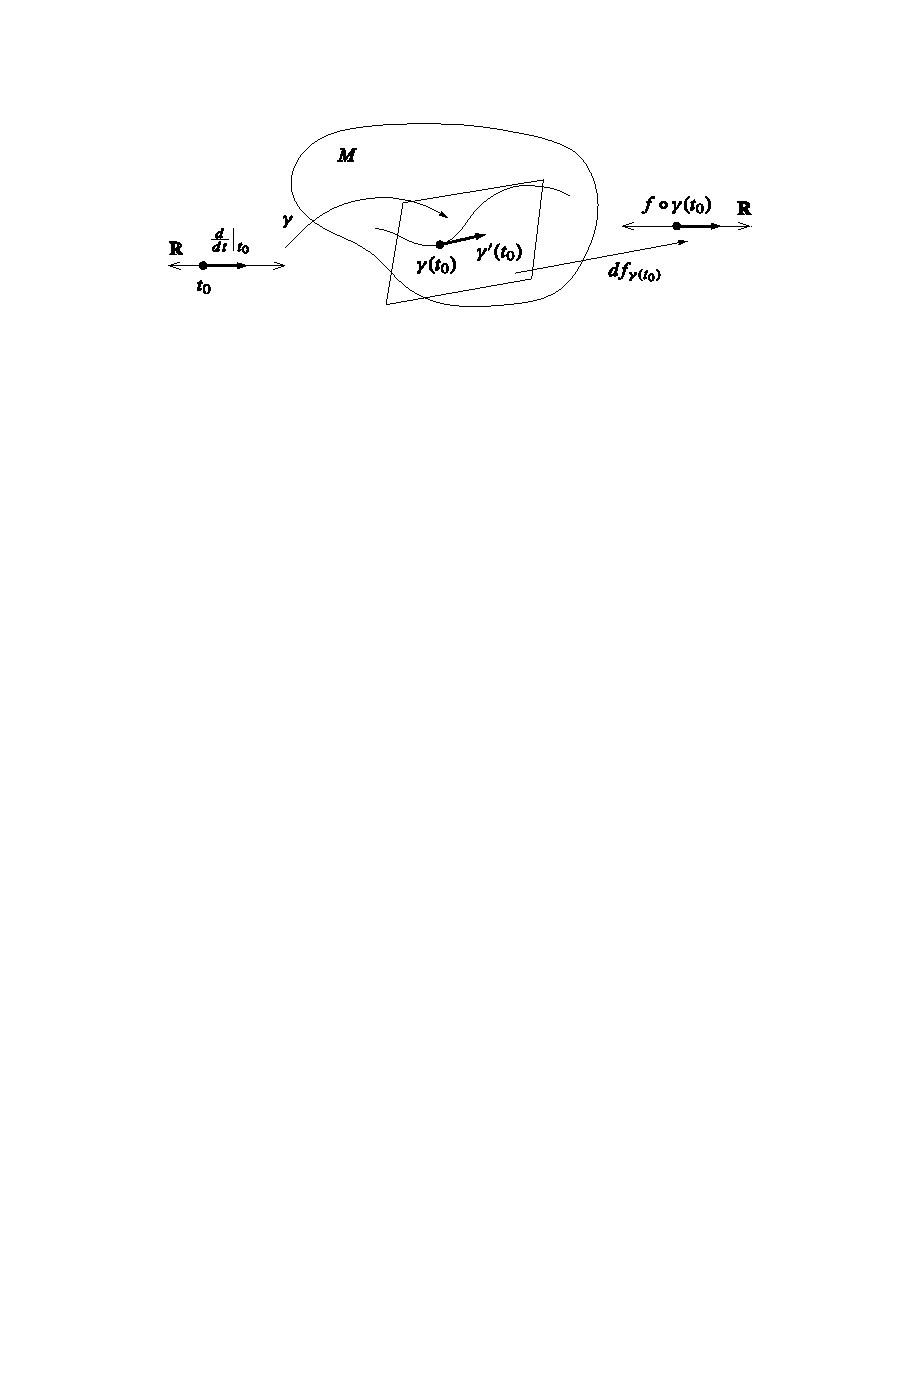
\includegraphics{diff-function}
\caption{Derivative of a function along a curve.}
\end{figure}
\begin{proof}
Directly from the definitions, for any $t_0\in J$,
\begin{align*}
df_{\gamma(t_0)}\big(\gamma'(t_0)\big)&=\gamma'(t_0)f=d\gamma_{t_0}\Big(\frac{d}{dt}\Big|_{t_0}\Big)f=\frac{d}{dt}\Big|_{t_0}(f\circ\gamma)=(f\circ\gamma)'(t_0)
\end{align*}
\end{proof}
You may have noticed that for a smooth real-valued function $f:M\to\R$, we now have two different definitions for the differential of $f$ at a point $p\in M$. In Section~\ref{tangent vector section}, we defined $df_p$ as a linear map from $Tp_M$ to $T_{f(p)}\R$. In this section, we defined $df_p$ as a covector at $p$, which is to say a linear map from $T_pM$ to $\R$. These are really the same object, once we take into account the canonical identification between $\R$ and $T_{f(p)}\R$; one easy way to see this is to note that both are represented in coordinates by the row matrix whose components are the partial derivatives of $f$: If $v=v^i\partial/\partial x^i|_p\in T_pM$, then
\[df_p(v)=df_p\Big(v^i\frac{\partial}{\partial x^i}\Big|_p\Big)=\frac{\partial f}{\partial x^i}(p)\frac{d}{dt}\Big|_{f(p)},\quad vf=v^i\frac{\partial}{\partial x^i}\Big|_pf=v^i\frac{\partial f}{\partial x^i}(p)\]\par
Similarly, if $\gamma$ is a smooth curve in $M$, we have two different meanings for the expression $(f\circ\gamma)'(t)$. On the one hand, $f\circ\gamma$ can be interpreted as a smooth curve in $\R$, and thus $(f\circ\gamma)'(t)$ is its velocity at the point $f\circ\gamma(t)$, which is an element of the tangent space $T_{f(t)}\R$. Proposition~\ref{diff composite curve} shows that this tangent vector is equal to $df_{\gamma(t)}\big(\gamma'(t)\big)$, thought of as an element of $T_{f(\gamma(t))}\R$. On the other hand, $f\circ\gamma$ can
also be considered simply as a real-valued function of one real variable, and then $(f\circ\gamma)'(t)$ is just its ordinary derivative. Proposition~\ref{diff function curve} shows that this derivative is equal to $df_{\gamma(t)}\big(\gamma'(t)\big)$, thought of as a real number. Which of these interpretations we choose depends on the purpose we have in mind.
\subsection{Pullbacks of covector fields}
As we have seen, a smooth map yields a linear map on tangent vectors called the differential. Dualizing this leads to a linear map on covectors going in the opposite
direction.\par
Let $F:M\to N$ be a smooth map between smooth manifolds with or without boundary, and let $p\in M$ be arbitrary. The differential $dF_p:T_pM\to T_{F(p)}N$ yields a dual linear map
\[df^*_p:T^*_{F(p)}N\to T^*_pM\]
called the (pointwise) pullback by $F$ at $p$, or the cotangent map of $F$. Unraveling the definitions, we see that $df^*_p$ is characterized by
\[df^*_p(\omega)(v)=\omega\big(dF_p(v)\big)\for \omega\in T^*_{F(p)}N,v\in T_pM\]
Given a smooth map $F:M\to N$ and a covector field $\omega$ on $N$, define a rough covector field $f^*\omega$ on $M$, called the pullback of $\omega$ by $F$, by
\[(f^*\omega)_p=df^*_p(\omega_{F(p)})\]
It acts on a vector $v\in T_pM$ by
\[(f^*\omega)_p(v)=\omega_{F(p)}\big(dF_p(v)\big)\]
\begin{proposition}\label{pull back functor}
Let $F:M\to N$ and $G:N\to P$ be smooth maps between smooth manifolds, then
\begin{itemize}
\item[(a)] $(G\circ F)^*=f^*\circ G^*$.
\item[(b)] $(\mathrm{id}_M)^*=\mathrm{id}_{T^*M}$.
\end{itemize}
\end{proposition}
\begin{proof}
Choose a point $p\in M$, let $\omega\in T^*_{F(G(p))}$ and $v\in T_pM$. Then 
\begin{align*}
\big((G\circ F)^*\omega\big)(v)&=\omega\big(d(G\circ F)_p(v)\big)=\omega\big(dG_{F(p)}\circ dF_{p}(v)\big)=(G^*\omega)\big(dF_p(v)\big)\\
&=\big(f^*(G^*\omega)\big)(v)=(f^*\circ G^*\omega)(v)
\end{align*}
Thus
\[(G\circ F)^*=f^*\circ G^*.\]
Now the second claim is obvious.
\end{proof}
In contrast to the vector field case, there is no ambiguity here about what point to pull back from: the value of $f^*\omega$ at $p$ is the pullback of $\omega$ at $F(p)$. We will show that $f^*\omega$ is continuous, and is smooth when $\omega$ is smooth. Before we do so, let us prove two important properties of the pullback.
\begin{proposition}\label{pull back prop}
Let $F:M\to N$ be a smooth map between smooth manifolds with or without boundary. Suppose $f$ is a continuous real-valued function on $N$, and $\omega$ is a covector field on $N$. Then
\begin{align}\label{pull back prop-1}
f^*(f\omega)=(f\circ F)f^*\omega
\end{align}
If in addition $f$ is smooth, then
\begin{align}\label{pull back prop-2}
f^*du=d(f\circ F)
\end{align}
\end{proposition}
\begin{proof}
We compute
\begin{align*}
\big(f^*(f\omega)\big)_p=df^*_p\big(f(F(p))\omega_{F(p)}\big)=f(F(p))df^*(\omega_{F(p)})=f\circ F(p)(f^*\omega)_p=\big((f\circ F)f^*\omega\big)_p
\end{align*}
and
\begin{align*}
(f^*df)_p(v)=\big(df^*_p(df_{F(p)})\big)(v)=df_{F(p)}(dF_p(v))=dF_p(v)(f)=v(f\circ F)=d(f\circ F)_p(v)
\end{align*}
\end{proof}
\begin{proposition}
Suppose $F:M\to N$ is a smooth map between smooth manifolds with or without boundary, and let $\omega$ be a covector field on $N$. Then $f^*\omega$ is a
$($continuous$)$ covector field on $M$. If $\omega$ is smooth, then so is $f^*\omega$.
\end{proposition}
\begin{proof}
Let $p\in M$ be arbitrary, and choose smooth coordinates $(y^j)$ for $N$ in a
neighborhood $V$ of $F(p)$. Let $U=F^{-1}(V)$, which is a neighborhood of $p$. Writing $\omega$ in coordinates as $\omega=\omega_jdy^j$ for continuous functions $\omega_j$ on $V$ and using Proposition~\ref{pull back prop} twice (applied to $F|_U$), we have the following computation in $U$:
\begin{align}\label{pull back-1}
f^*\omega=f^*(\omega_jdy^j)=(\omega_j\circ F)f^*dy^j=(\omega_j\circ F)d(y^j\circ F)
\end{align}
This expression is continuous, and is smooth if $\omega$ is smooth.
\end{proof}
Formula $(\ref{pull back-1})$ for the pullback of a covector field can also be written in the following way:
\begin{align}\label{pull back-2}
f^*\omega=(\omega_j\circ F)d(y^j\circ F)=(\omega_j\circ F)dF^j
\end{align}
where $F^j$ is the $j$-th component function of $F$ in these coordinates. Using either of these formulas, the computation of pullbacks in coordinates is exceedingly simple, as the next example shows.
\begin{example}
Let $F:\R^3\to\R^2$ be the map given by
\[(u,v)=F(x,y,z)=(x^2y,y\sin z)\]
and let $\omega\in\X^*(\R^2)$ be the covector field
\[\omega=udv+vdu\]
According to $(\ref{pull back-1})$, the pullback $f^*$ is given by
\begin{align*}
f^*\omega&=(u\circ F)d(v\circ F)+(v\circ F)d(u\circ F)=(x^2y)\,d(y\sin z)+(y\sin z)\,d(x^2y)\\
&=x^2y(\sin z\,dy+y\cos z\,dz)+(y\sin z)(2xy\,dx+x^2\,dy)\\
&=2xy^2\sin z\,dx+2x^2y\sin z\,dy+x^2y^2\cos z\,dz
\end{align*}
\end{example}
In other words, to compute $f^*$, all we need to do is substitute the component
functions of $F$ for the coordinate functions of $N$ everywhere they appear in $\omega$. This also yields an easy way to remember the transformation law for a covector field under a change of coordinates. Again, an example will convey the idea better than a general formula.
\begin{example}
Let $(r,\theta)$ be polar coordinates on, say, the right half-plane $H=\{(x,y):x>0\}$. We can think of the change of coordinates $(x,y)=(r\cos\theta,r\sin\theta)$ as the coordinate expression for the identity map of $H$, but using $(r,\theta)$ as coordinates for the domain and $(x,y)$ for the codomain. Then the pullback formula tells us that we can compute the polar coordinate expression for a covector field simply by substituting $x=r\cos\theta,y=r\sin\theta$ and expanding. For example,
\begin{align*}
x\,dy-y\,dx&=r\cos\theta\,d(r\sin\theta)-r\sin\theta\,d(r\cos\theta)\\
&=r\cos\theta(\sin\theta\,dr+r\cos\theta\,d\theta)-r\sin\theta(\cos\theta\,dr-r\sin\theta\,d\theta)\\
&=r\cos\theta\sin\theta\,dr+r^2\cos\theta^2\,d\theta-r\sin\theta\cos\theta\,dr+r^2\sin\theta^2\,d\theta\\
&=r^2d\theta
\end{align*}
\end{example}
\subsubsection{Restricting covector fields to submanifolds}
In Section~\ref{vector field section}, we considered the conditions under which a vector field restricts to a submanifold. The restriction of covector fields to submanifolds is much simpler.\par
Suppose $M$ is a smooth manifold with or without boundary, $S\sub M$ is an immersed submanifold with or without boundary, and $\iota:S\hookrightarrow M$ is the inclusion map. If $\omega$ is any smooth covector field on $M$, the pullback by $\iota$ yields a smooth covector field $\iota^*\omega$ on $S$. To see what this means, let $v\in T_pS$ be arbitrary, and compute
\[(\iota^*\omega)_p(v)=d\iota^*_p(\omega)(v)=\omega_p\big(d\iota_p(v)\big)=\omega_p(v)\]
since $d\iota_p:T_pS\to T_pM$ is just the inclusion map, under our usual identification of $T_pS$ with a subspace of $T_pM$. Thus, $\iota^*$ is just the restriction of $\omega$ to vectors tangent to $S$. For this reason, $\iota^*\omega$ is often called the \textbf{restriction of $\bm{\iota}$ to $\bm{S}$}. Be warned, however, that $\iota^*\omega$ might equal zero at a given point of $S$, even though considered as a covector field on $M$, $\omega$ might not vanish there. An example will help to clarify this distinction.
\begin{example}
Let $\omega=dy$ on $\R^2$, and let $S$ be the $x$-axis, considered as an embedded submanifold of $\R^2$. As a covector field on $\R^2$, $\omega$ is nonzero everywhere, because one of its component functions is always $1$. However, the restriction $\iota^*\omega$ is identically zero, because $y$ vanishes identically on $S$:
\[\iota^*\omega=d(y\circ\iota)=0\]
\end{example}
To distinguish the two ways in which we might interpret the statement $\iota$ vanishes on $S$, one usually says that \textbf{$\bm{\omega}$ vanishes along $\bm{S}$} or \textbf{vanishes at points of $\bm{S}$} if $\omega_p=0$ for every point $p\in S$. The weaker condition that $\iota^*\omega=0$ is expressed by saying that \textbf{the restriction of $\bm{\omega}$ to $\bm{S}$ vanishes}, or \textbf{the pullback of $\bm{\omega}$ to $\bm{S}$ vanishes}.
\begin{proposition}\label{diff restrict submani}
Suppose $M$ is a smooth manifold with or without boundary and $S\sub M$ is an immersed submanifold with or without boundary. For any $f\in C^\infty(M)$ we have $d(f|_S)=\iota^*(df)$. Thus the pullback of $df$ to $S$ is zero if and only if $f$ is constant on each component of $S$.
\end{proposition}
\begin{proof}
Let $p\in S$ and choose $v\in T_pM$, we compute that
\[\big(\iota^*(df)\big)_p(v)=df\big(d\iota_p(v)\big)=d\iota_p(v)(f)=v(f\circ\iota)=v(f|_S)=d(f|_S)(v)\]
Thus $\iota^*(df)=0$ if and only if $d(f|_S)=0$, and the second claim follows from Proposition~\ref{diff vanish}.
\end{proof}
\subsection{Line integrals}
Another important application of covector fields is to make coordinate-independent sense of the notion of a line integral.\par
We begin with the simplest case: \textit{an interval in the real line}. Suppose $[a,b]\sub\R$ is a compact interval, and $\omega$ is a smooth covector field on $[a,b]$. (This means that the component function of $\omega$ admits a smooth extension to some neighborhood of $[a,b]$) If we let $t$ denote the standard coordinate on $\R$, then $\omega$ can be written $\omega_t=f(t)dt$ for some smooth function $f:[a,b]\to\R$. We define the \textbf{integral of $\bm{\omega}$ over $\bm{[a,b]}$} to be
\[\int_{[a,b]}\omega=\int_{a}^{b}f(t)dt\]
The next proposition should convince you that this is more than just a trick of
notation.
\begin{proposition}[\textbf{Diffeomorphism Invariance of the Integral}]\label{diffeo invariance integral}
Let $\omega$ be a smooth covector field on the compact interval $[a,b]\sub\R$. If $\varphi:[c,d]\to[a,b]$ is an increasing diffeomorphism, then
\[\int_{[c,d]}\varphi^*\omega=\int_{[a,b]}\omega\]
\end{proposition}
\begin{proof}
If we let $s$ denote the standard coordinate on $[c,d]$ and $t$ that on $[a,b]$, then $(\ref{pull back-2})$ shows that the pullback $\varphi^*\omega$ has the coordinate expression 
\[(\varphi^*\omega)_s=f\circ\varphi(s)\,d\varphi(s)=f\circ\varphi(s)\varphi'(s)\,ds.\] 
Inserting this into the definition of the line integral and using the
change of variables formula for ordinary integrals, we obtain
\[\int_{[c,d]}\varphi^*\omega=\int_{c}^{d}f\circ\varphi(s)\varphi'(s)\,ds=\int_{a}^{b}f(t)dt=\int_{[a,b]}\omega\]
\end{proof}
\begin{remark}\label{diffeo invariance remk}
If $\varphi:[c,d]\to[a,b]$ is a decreasing diffeomorphism, then
\[\int_{[c,d]}\varphi^*\omega=-\int_{[a,b]}\omega\]
\end{remark}
Now let $M$ be a smooth manifold with or without boundary. By a \textbf{curve segment} in $M$ we mean a continuous curve $\gamma:[a,b]\to M$ whose domain is a compact interval. It is a smooth curve segment if it is smooth when $[a,b]$ is considered as a manifold with boundary. It is a \textbf{piecewise smooth curve segment} if there exists a finite partition 
\[a=a_0<a_1<\cdots<a_k=b\]
such that $\gamma|_{[a_{i-1},a_i]}$ is smooth for each $i$. Continuity of $\gamma$ means that $\gamma(t)$ approaches the same value as t approaches any of the points $a_i$ (other than $a_0$ or $a_n$) from the left or the right. Smoothness of $\gamma$ on each subinterval means that $\gamma$ has one-sided velocity vectors at each such $a_i$ when approaching from the left or the right, but these one-sided velocities need not be equal.
\begin{proposition}\label{connect by smooth curve}
If $M$ is a connected smooth manifold with or without boundary, any two points of $M$ can be joined by a piecewise smooth curve segment.
\end{proposition}
\begin{proof}
Let $p$ be an arbitrary point of $M$, and define a subset
\[\mathscr{C}=\{q\in M:\text{ there is a piecewise smooth curve segment in $M$ from $p$ to $q$}\}\]
Clearly, $p\in\mathscr{C}$, so $\mathscr{C}$ is nonempty. To show that $\mathscr{C}=M$, we need to show that it is open and closed in $M$.\par
Let $q\in \mathscr{C}$ be arbitrary, which means that there is a piecewise smooth curve segment $\gamma$ going from $p$ to $q$. Let $U$ be a smooth coordinate ball (or half-ball) centered at $q$. If $q'$ is any point in $U$, then it is easy to construct a piecewise smooth curve segment from $p$ to $q'$ by first following $\gamma$ from $p$ to $q$, and then following a straight-line
path in coordinates from $q$ to $q'$. Thus $U\sub\mathscr{C}$, which shows that $\mathscr{C}$ is open in $M$.\par
On the other hand, if $q$ is a limit point of $\mathscr{C}$, let $U$ be a smooth coordinate ball or half-ball around $q$ as above. Then there is some point $q'\in\mathscr{C}\cap U$. In this case, we can construct a piecewise smooth curve from $p$ to $q$ by first following one from $p$ to $q'$ and then following a straight-line path in coordinates from $q'$ to $q$. This shows that $q\in\mathscr{C}$, so $\mathscr{C}$ is also closed.
\end{proof}
If $\gamma:[a,b]\to M$ is a smooth curve segment and $\omega$ is a smooth covector field on $M$, we define the \textbf{line integral of $\bm{\omega}$ over $\bm{\gamma}$} to be the real number
\[\int_{\gamma}\omega=\int_{a}^{b}\gamma^*\omega\]
Because $\gamma^*\omega$ is a smooth covector field on $[a,b]$, this definition makes sense. More generally, if $\gamma$ is piecewise smooth, we define
\[\int_{\gamma}\omega=\sum_{i=1}^{k}\int_{[a_{i-1},a_i]}\gamma^*\omega\]
where $[a_{i-1},a_i],1\leq i\leq k$ are subintervals on which $\gamma$ is smooth.
\begin{proposition}[\textbf{Properties of Line Integrals}]\label{line integral prop}
Let $M$ be a smooth manifold with or without boundary. Suppose $\gamma:[a,b]\to M$ is a piecewise smooth curve segment, and $\omega_1,\omega_2\in\X^*(M)$.
\begin{itemize}
\item[(a)] For any $c_1,c_2\in\R$,
\[\int_{\gamma}(c_1\omega_1+c_2\omega_2)=c_1\int_{\gamma}\omega_1+c_2\int_{\gamma}\omega_2.\]
\item[(b)] If $\gamma$ is a constant map, then $\int_\gamma\omega=0$.
\item[(c)] If $\gamma_1=\gamma|_{[a,c]}$ and $\gamma_1=\gamma|_{[c,b]}$ with $a<c<b$, then
\[\int_{\gamma}\omega=\int_{\gamma_1}\omega+\int_{\gamma_2}\omega.\]
\item[(d)] If $F:M\to N$ is any smooth map and $\eta\in\X^*(N)$, then
\[\int_{\gamma}f^*\eta=\int_{F\circ\gamma}\eta.\]
\end{itemize}
\end{proposition}
\begin{proof}
We only prove the last equality:
\begin{align*}
\int_{\gamma}f^*\eta=\int_{a}^{b}\gamma^*(f^*\eta)=\int_{a}^{b}(F\circ\gamma)^*\eta=\int_{F\circ\gamma}\eta.
\end{align*}
where we use Proposition~\ref{pull back functor}.
\end{proof}
\begin{example}\label{covector closed not exact eg}
Let $M=\R^2-\{0\}$, let $\omega$ be the covector field on $M$ given by
\[\omega=\frac{x\,dy-y\,dx}{x^2+y^2}\]
and let $\gamma:[0,2\pi]\to M$ be the curve segment defined by $\gamma(t)=(\cos t,\sin t)$. Since $\gamma^*\omega$ can be computed by substituting $x=\cos t$ and $y=\sin t$ everywhere in the formula for $\omega$, we find that
\[\int_{\gamma}\omega=\int_{0}^{2\pi}\frac{\cos t\,d\sin t-\sin t\,d\cos t}{\cos^2t+\sin^2t}=\int_{0}^{2\pi}dt=2\pi\]
\end{example}
One of the most significant features of line integrals is that they are independent of parametrization, in a sense we now make precise. If $\gamma:[a,b]\to M$ and $\widetilde{\gamma}:[c,d]\to M$ are piecewise smooth curve segments, we say that $\widetilde{\gamma}$ is a reparametrization of $\gamma$ if $\widetilde{\gamma}=\gamma\circ\varphi$ for some diffeomorphism $\varphi:[c,d]\to[a,b]$. If $\varphi$ is an increasing function, we say that $\widetilde{\gamma}$ is a \textbf{forward reparametrization}, and if $\varphi$
is decreasing, it is a \textbf{backward reparametrization}. (More generally, with obvious modifications one can allow $\varphi$ to be piecewise smooth.)
\begin{proposition}[\textbf{Parameter Independence of Line Integrals}]\label{line integral para independent}
Suppose $M$ is a smooth manifold with or without boundary, $\omega\in\X^*(M)$, and $\gamma$ is a piecewise smooth curve segment in $M$. For any reparametrization $\widetilde{\gamma}$ of $\gamma$, we have
\[\int_{\widetilde{\gamma}}\omega=\begin{cases}
\quad\displaystyle{\int_{\gamma}\omega}&\text{if $\widetilde{\gamma}$ is a forward reparametrization},\\[8pt]
-\displaystyle{\int_{\gamma}\omega}&\text{if $\widetilde{\gamma}$ is a backward reparametrization}.
\end{cases}\]
\end{proposition}
\begin{proof}
First assume that $\gamma:[a,b]\to M$ is smooth, and suppose $\widetilde{\gamma}=\gamma\circ\varphi$, where $\varphi$ is an increasing diffeomorphism. Then Proposition~\ref{diffeo invariance integral} and ~\ref{pull back prop} imply
\[\int_{\widetilde{\gamma}}=\int_{c}^{d}(\gamma\circ\varphi)^*\omega=\int_{c}^{d}\varphi^*\circ\gamma^*\omega=\int_{a}^{b}\gamma^*\omega=\int_{\gamma}\omega\]
When $\varphi$ is decreasing, the analogous result follows from Remark~\ref{diffeo invariance remk}. If $\gamma$ is only piecewise smooth, the result follows simply by applying the preceding argument on each subinterval where $\gamma$ is smooth.
\end{proof}
The next proposition gives a useful alternative expression for a line integral.
\begin{proposition}\label{line integral ordinary form}
If $\gamma:[a,b]\to M$ is a piecewise smooth curve segment, the line integral of $\omega$ over $\gamma$ can also be expressed as the ordinary integral
\[\int_\gamma\omega=\int_{a}^{b}\omega_{\gamma(t)}\big(\gamma'(t)\big)dt\]
\end{proposition}
\begin{proof}
First suppose that $\gamma$ is smooth and that its image is contained in the domain of a single smooth chart. If the coordinate representations of $\gamma$ is $(\gamma^1(t),\dots,\gamma^n(t))$, then
\[\gamma'(t)=\dot{\gamma}^j(t)\frac{\partial}{\partial x^j}\Big|_{\gamma(t)}\] 
If we write $\omega=\omega_idx^i$, then
\[\omega_{\gamma(t)}\big(\gamma'(t)\big)=(\omega_i\circ\gamma)(t)\,dx^i\Big(\dot{\gamma}^j(t)\frac{\partial}{\partial x^j}\Big|_{\gamma(t)}\Big)=(\omega_i\circ\gamma)(t)\dot{\gamma}^i(t).\]
Combining this with the coordinate formula $(\ref{pull back-2})$ for the pullback, we obtain
\begin{align*}
(\gamma^*\omega)_t=(\omega_i\circ\gamma)(t)\,d\gamma^i(t)=(\omega_i\circ\gamma)(t)\dot{\gamma}^i(t)dt=\omega_{\gamma(t)}\big(\gamma'(t)\big)dt.
\end{align*}
Therefore, by the definition of the line integral,
\[\int_{\gamma}\omega=\int_{a}^{b}\gamma^*\omega=\int_{a}^{b}\omega_{\gamma(t)}\big(\gamma'(t)\big)dt.\]
If $\gamma$ is an arbitrary smooth curve segment, by compactness there exists a finite partition 
\[a=a_0<a_1<\cdots<a_k=b\] 
such that $\gamma([a_{i-1},a_i])$ is contained in the domain of a single smooth chart for each $i$, so we can apply the computation above on each such subinterval. Finally, if $\gamma$ is only piecewise smooth, we simply apply the same argument on each subinterval on which $\gamma$ is smooth.
\end{proof}
There is one special case in which a line integral is trivial to compute: the line integral of a differential.
\begin{proposition}[\textbf{Fundamental Theorem for Line Integrals}]\label{line integral fundamental thm}
Let $M$ be a smooth manifold with or without boundary. Suppose $f$ is a smooth real-valued function on $M$ and $\gamma:[a,b]\to M$ is a piecewise smooth curve segment in $M$. Then
\[\int_{\gamma}df=f(\gamma(b))-f(\gamma(a))\]
\end{proposition}
\begin{proof}
Suppose first that $\gamma$ is smooth. By Propositions~\ref{diff function curve} and ~\ref{line integral ordinary form},
\[\int_\gamma df=\int_{a}^{b}df_{\gamma(t)}\big(\gamma'(t)\big)dt=\int_{a}^{b}(f\circ\gamma)'(t)dt=f(\gamma(b))-f(\gamma(a))\]
by the fundamental theorem of calculus.\par
If $\gamma$ is merely piecewise smooth, let 
\[a=a_0<a_1<\cdots<a_k=b\] 
be the endpoints of the subintervals on which $\gamma$ is smooth. Applying the above argument on each subinterval and summing, we find that
\[\int_\gamma df=\sum_{i=1}^{k}\int_{a_{i-1}}^{a_i}\big(f(\gamma(a_{i-1}))-f(\gamma(a_i))\big)=f(\gamma(b))-f(\gamma(a))\]
because the contributions from all the interior points cancel.
\end{proof}
\subsection{Conservative covector fields}
Theorem~\ref{line integral fundamental thm} shows that the line integral of any covector field that can be written as the differential of a smooth function can be computed easily once the smooth function is known. For this reason, there is a special term for covector fields with this property. A smooth covector field $\omega$ on a smooth manifold $M$ with or without boundary is said to be \textbf{exact} (or an \textbf{exact differential}) on $M$ if there is a function $f\in C^\infty(M)$ such that $\omega=df$. In this case, the function $f$ is called a \textbf{potential} for $\omega$.\par
The potential is not uniquely determined, but by Proposition~\ref{diff vanish}, the difference between any two potentials for $\omega$ must be constant on each component of $M$. Because exact differentials are so easy to integrate, it is important to develop criteria for deciding whether a covector field is exact. Theorem~\ref{line integral fundamental thm} provides an important clue. It shows that the line integral of an exact covector field depends only on the endpoints $p=\gamma(a)$ and $q=\gamma(b)$: any other curve segment from $p$ to $q$ would give the same value for the line integral. In particular, if $\gamma$ is a \textbf{closed curve segment}, meaning that $\gamma(a)=\gamma(b)$, then the integral of $df$ over $\gamma$ is zero.\par
We say that a smooth covector field $\omega$ is \textbf{conservative} if the line integral of $\omega$ over every piecewise smooth closed curve segment is zero.\par
Conservative covector fields can also be characterized by path independence.
\begin{proposition}
A smooth covector field $\omega$ is conservative if and only if its line integrals are path-independent, in the sense that $\int_\gamma\omega=\int_{\widetilde{\gamma}}\omega$ whenever $\gamma$ and $\widetilde{\gamma}$ are piecewise smooth curve segments with the same starting and ending points.
\end{proposition}
\begin{proof}
If $\gamma:[a,b]\to M$ and $\widetilde{\gamma}:[c,d]\to M$ are piecewise smooth curve segments with the same starting and ending points, we define $\gamma-\widetilde{\gamma}:[-1,1]$ to be the curve
\[(\gamma-\widetilde{\gamma})(t)=\begin{cases}
\gamma\big(a+(b-a)(t+1)\big)&t\in[-1,0]\\
\widetilde{\gamma}\big(d-(d-c)t\big)&t\in[0,1]
\end{cases}\]
Geomrtrically speaking, $\gamma-\widetilde{\gamma}$ is defined by first travel along $\gamma$ forward, then along $\widetilde{\gamma}$ backward. Then $\gamma-\widetilde{\gamma}$ is piecewise smooth and closed, and we have the observation
\[\int_{\gamma-\widetilde{\gamma}}\omega=\int_{\gamma}\omega-\int_{\widetilde{\gamma}}\omega\]
Now the claim is clear.
\end{proof}
\begin{proposition}\label{covector conservative iff exact}
Let $M$ be a smooth manifold with or without boundary. A smooth covector field on $M$ is conservative if and only if it is exact.
\end{proposition}
\begin{proof}
If $\omega\in\X^*(M)$ is exact, Theorem~\ref{line integral fundamental thm} shows that it is conservative, so we need only prove the converse. Suppose $\omega$ is conservative, and assume for the moment that $M$ is connected. Because the line integrals of $\omega$ are path-independent, we can adopt the following notation: for any points $p,q$ we use the notation $\int_p^q\omega$ to denote the value of any line integral of the form $\int_\gamma\omega$, where $\gamma$ is a piecewise smooth curve segment from $p$ to $q$. Because a backward reparametrization of a path from $p$ to $q$ is a path from $q$ to $p$, Proposition~\ref{line integral para independent} implies $\int_q^p\omega=-\int_p^q\omega$ and for any three points $p_1,p_2,p_3\in M$ Proposition~\ref{line integral prop}(c) implies that
\begin{align}\label{covector conservative-1}
\int_{p_1}^{p_3}\omega=\int_{p_1}^{p_2}\omega+\int_{p_2}^{p_3}\omega
\end{align}
Now choose any base point $p_0\in M$, and define a function $f:M\to\R$ by
\[f(q)=\int_{p_0}^{p}\omega\]
We prove that $f$ is smooth and $df=\omega$.\par 
To accomplish this, let $q_0\in M$ be arbitrary, let $(U,(x^i))$ be a smooth chart centered at $q_0$, and write the coordinate representation of $\omega$ in $U$ as $\omega=\omega_idx^i$. We need to show that
\[\frac{\partial f}{\partial x^j}(q_0)=\omega_j(q_0)\for 1\leq j\leq n\]
First suppose $q_0\in\Int M$. Fix $j$, and let $\gamma:[-\eps,\eps]\to U$ be the smooth curve segment defined in coordinates by $\gamma(t)=(0,\dots,t,\dots,0)$, with $t$ in the $j$-th place, and with $\eps$ chosen small enough that $\gamma([-\eps,\eps])\sub U$. Let $p_1=\gamma(-\eps)$, and define a new function $\widetilde{f}:M\to\R$ by $\widetilde{f}(q)=\int_{p_1}^{q}\omega$. Note that $(\ref{covector conservative-1})$ implies that for all $q\in M$,
\[f(q)-\widetilde{f}(q)=\int_{p_0}^{q}\omega-\int_{p_1}^{q}\omega=\int_{p_0}^{p_1}\omega\]
which does not depend on $q$. Thus $\widetilde{f}$ and $f$ differ by a constant, so it suffices to show that $\partial\widetilde{f}/\partial x^j(q_0)=\omega_j(q_0)$.\par
Now $\gamma'(t)=\partial/\partial x^j|_{\gamma(t)}$ by construction, so 
\[\omega_{\gamma(t)}\big(\gamma'(t)\big)=\omega_{\gamma(t)}\Big(\frac{\partial}{\partial x^j}\Big|_{\gamma(t)}\Big)=\omega_j\big(\gamma(t)\big)\]
Since the restriction of $\gamma$ to $[-\eps,t]$ is a smooth curve from $p_1$ to $\gamma(t)$, we have
\[\widetilde{f}\circ\gamma(t)=\int_{p_1}^{\gamma(t)}\omega=\int_{-\eps}^{t}\omega_{\gamma(t)}\big(\gamma'(t)\big)=\int_{-\eps}^{t}\omega_j\big(\gamma(s)\big)ds\]
Thus, by the fundamental theorem of calculus,
\begin{align*}
\frac{\partial\widetilde{f}}{\partial x^j}(q_0)=\gamma'(0)\widetilde{f}=\frac{d}{dt}\Big|_{t=0}\widetilde{f}\circ\gamma(t)=\frac{d}{dt}\Big|_{t=0}\int_{-\eps}^{t}\omega_j\big(\gamma(s)\big)ds=\omega_j\big(\gamma(0)\big)=\omega_j(q_0)
\end{align*}
This shows that $df_{q_0}=\omega_{q_0}$ when $q_0\in\Int M$.\par
For $q_0\in\partial M$, the chart $(U,(x^i))$ is a boundary chart centered at $q_0$. The proof above shows that $\partial f/\partial x^j(q_0)=\omega_j(q_0)$ except in the case $j=n=\dim M$; but that case requires a special argument because $x^n$ takes on only nonnegative values in a boundary chart. In that case we simply set $p_1=\gamma(0)$ instead of $p_1=\gamma(-\eps)$, and proceed as before. Then the same argument shows that $df_{q_0}=\omega_{q_0}$ in this case as well. This completes the proof that $df=\omega$ when $M$ is connected. Since the component functions of $\omega$ are smooth and equal to the partial derivatives of $f$ in coordinates, this also shows that $f$ is smooth.\par
Finally, if $M$ is not connected, let $\{M_i\}$ be the components of $M$. The argument above shows that for each $i$ there is a function $f^i\in C^\infty(M)$ such that $df_i=\omega$ on $M_i$. Letting $f:M\to\R$ be the function that is equal to $f_i$ on $M_i$ for each $i$, we have $df=\omega$, thus completing the proof.
\end{proof}
\begin{example}
The covector field $\omega$ of Example~\ref{covector closed not exact eg} cannot be exact on $\R^2-\{0\}$, because it is not conservative: the computation in that example showed that $\int_\gamma\omega=2\pi\neq 0$, where $\gamma$ is the unit circle traversed counterclockwise.
\end{example}
To see a sufficient condition for exactness, suppose $\omega\in\X^*(M)$ is exact. Let $f$ be any potential function for $\omega$, and let $(U,(x^i))$ be any smooth chart on $M$. Because $f$ is smooth, it satisfies the following identity on $U$:
\begin{align*}
\frac{\partial^2f}{\partial x^i\partial x^j}=\frac{\partial^2f}{\partial x^j\partial x^i}
\end{align*}
Writing $\omega=\omega_idx^i$ in coordinates, we see that $\omega=df$ is equivalent to $\omega_i=\partial f/\partial x^i$. Substituting this, we find that the component functions of $\omega$ satisfy the following identity for each pair of indices $i$ and $j$:
\begin{align}\label{covector closed-1}
\frac{\partial\omega_i}{\partial x^j}=\frac{\partial\omega_j}{\partial x^i}
\end{align}
We say that a smooth covector field $\omega$ is closed if its components in every smooth chart satisfy $(\ref{covector closed-1})$. The following proposition summarizes the computation above.
\begin{proposition}
Every exact covector field is closed.
\end{proposition}
One technical difficulty in checking directly from the definition that a covector field is closed is that it would require checking that $(\ref{covector closed-1})$ holds in every coordinate chart. The next proposition gives an alternative characterization of closed covector fields that is coordinate independent, and incidentally shows that it suffices to check $(\ref{covector closed-1})$ in some coordinate chart around each point.
\begin{proposition}\label{covector closed iff}
Let $\omega$ be a smooth covector field on a smooth manifold $M$ with or without boundary. The following are equivalent:
\begin{itemize}
\item[(a)] $\omega$ is closed.
\item[(b)] $\omega$ satisfies $(\ref{covector closed-1})$ in some smooth chart around every point.
\item[(c)] For any open subset $U\sub M$ and smooth vector fields $X,Y\in\X(U)$,
\begin{align}\label{covector closed-2}
X(\omega(Y))-Y(\omega(X))=\omega([X,Y])
\end{align}
\end{itemize}
\end{proposition}
\begin{proof}
We will prove that $(a)\Rightarrow(b)\Rightarrow(c)\Rightarrow(a)$. The implication $(a)\Rightarrow(b)$ is immediate from the definition of closed covector fields.\par
To prove $(b)\Rightarrow(c)$, assume (b) holds, and suppose $U\sub M$ and $X,Y\in\X(U)$ as in the statement of (c). It suffices to verify that $(\ref{covector closed-2})$ holds in a neighborhood of each point of $U$. In any coordinate chart $(V,(x^i))$ with $V\sub U$, we can write $\omega=\omega_idx^i$, $X=X^j\partial/\partial x^j$ and $Y=Y^k\partial/\partial x^k$, and compute
\begin{align*}
X(\omega(Y))=X(\omega_iY^i)=Y^iX\omega_i+\omega_iXY^i=Y^iX^j\frac{\partial\omega_i}{\partial x^j}+\omega_iXY^i
\end{align*}
If we repeat the same computation with $X$ and $Y$ reversed and subtract, the terms involving derivatives of $\omega_i$ cancel by virtue of $(\ref{covector closed-1})$. Thus we get
\[X(\omega(Y))-Y(\omega(X))=\omega(XY^i-YX^i)\]
Formula $(\ref{Lie bracket-2})$ shows that this last expression is equal to $\omega([X,Y])$.\par
Finally, if $\omega$ satisfies (c), in any coordinate chart we can apply $(\ref{covector closed-1})$ with $X=\partial/\partial x^i$ and $\partial/\partial x^j$, noting that $[X,Y]=0$ in that case, to obtain $(\ref{covector closed-2})$.
\end{proof}
One consequence of this proposition is that closedness can be easily checked
using criterion (b), so many covector fields can be shown quickly not to be exact because they are not closed. Another is the following corollary.
\begin{corollary}
Suppose $F:M\to N$ is a local diffeomorphism. Then the pullback $f^*:\X^*(N)\to\X^*(M)$ takes closed covector fields to closed covector fields,
and exact ones to exact ones.
\end{corollary}
\begin{proof}
The result for exact covector fields follows immediately from $(\ref{pull back prop-2})$. For closed covector fields, if $(U,\varphi)$ is any smooth chart for $N$, then $\varphi\circ F$ is a smooth chart for $M$ in a neighborhood of each point of $F^{-1}$. In these coordinates, the coordinate representation of $F$ is the identity, so if $\omega$ satisfies $(\ref{covector closed-1})$ in $U$, then $f^*\omega$ satisfies $(\ref{covector closed-1})$ in $F^{-1}(U)$.
\end{proof}
\begin{example}
Consider the following covector field on $\R^2$:
\[\omega=y\cos xy\,dx+x\cos yx\,dy\]
It is easy to check that
\[\frac{\partial(y\cos xy)}{\partial y}=\frac{\partial(x\cos xy)}{\partial x}=\cos xy-xy\sin xy\]
so $\omega$ is closed. In fact, $\omega=d(\sin xy)$.\par
On the other hand, the covector field
\[\eta=x\cos xy\,dx+y\cos xy\,dy\]
is not closed, because
\[\frac{\partial(x\cos xy)}{\partial y}=-x^2\sin xy,\quad \frac{\partial(y\cos xy)}{\partial x}=-y^2\sin xy.\]
Thus $\eta$ is not exact.
\end{example}
However, not every closed covector field is exact. It turns out that this question depends in a subtle way on the shape of the domain, as the next example illustrates.
\begin{example}
Look once again at the covector field $\omega$ of Example~\ref{covector closed not exact eg}. A straightforward computation shows that $\omega$ is closed; but as we observed above, it is not exact on $\R^2-\{0\}$. On the other hand, if we restrict the domain to the right half-plane $U=\{(x,y):x>0\}$, a computation shows that $\omega=d\arctan(y/x)$ there. This can be seen more clearly in polar coordinates, where $\omega=d\theta$. The problem, of course, is that there is no smooth $($or even continuous$)$ angle function on all of $\R^2-\{0\}$, which is a consequence of the hole in the center.
\end{example}
This last example illustrates a key principle: the question of whether a particular closed covector field is exact is a global one, depending on the shape of the domain in question. This observation is the starting point for de Rham cohomology, which expresses a deep relationship between smooth structures and topology.\par
If $V$ is a finite-dimensional vector space, a subset $U\sub V$ is said to be star-shaped if there is a point $c\in U$ such that for every $x\in U$, the line segment from $c$ to $x$ is entirely contained in $U$. For example, every convex subset is star-shaped.
\begin{theorem}[\textbf{Poincar\'e Lemma for Covector Fields}]\label{Poincare lemma}
If $U$ is a star-shaped open subset of $\R^n$ or $\H^n$, then every closed covector field on $U$ is exact.
\end{theorem}
\begin{proof}
Suppose $U$ is star-shaped with respect to $c\in U$, and let $\omega=\omega_idx^i$ be a closed covector field on $U$. As in the proof of Theorem~\ref{covector conservative iff exact}, we will construct a potential function for $\omega$ by integrating along smooth curve segments from $c$. However, in this case we do not know a priori that the line integrals are path-independent, so we must integrate along specific paths.\par
Because diffeomorphisms take closed forms to closed forms and exact ones to
exact ones, we can apply a translation to $U$ to arrange that $c=0$. For any point $x\in U$, let $\gamma_x:[0,1]\to U$ denote the line segment from $0$ to $x$, parametrized as $\gamma_x(t)=tx$. The hypothesis guarantees that the image of $\gamma_x$ lies entirely in $U$ for each $x\in U$. Define a function $f:U\to\R$ by
\[f(x)=\int_{\gamma_x}\omega\]
We need to show that $\partial/\partial x^j$ for $1\leq j\leq n$. To begin, we compute
\begin{align}\label{Poincare lemma construction}
f(x)=\int_{0}^{1}\omega_{\gamma_x(t)}\big(\gamma_x'(t)\big)dt=\int_{0}^{1}\omega_i(tx)x^idt.
\end{align}
To compute the partial derivatives of $f$, we note that the integrand is smooth in all variables, so it is permissible to differentiate under the integral sign to obtain
\[\frac{\partial f}{\partial x^j}(x)=\int_{0}^{1}\Big(t\frac{\partial\omega_i}{\partial x^j}(tx)x^i+\omega_j(tx)\Big)dt\]
Because $\omega$ is closed, this reduces to
\begin{align*}
\frac{\partial f}{\partial x^j}(x)&=\int_{0}^{1}\Big(t\frac{\partial\omega_i}{\partial x^j}(tx)x^i+\omega_j(tx)\Big)dt=\int_{0}^{1}\Big(t\frac{\partial\omega_j}{\partial x^i}(tx)x^i+\omega_j(tx)\Big)dt\\
&=\int_{0}^{1}\frac{d}{dt}\big(t\omega_j(tx)\big)dt=\Big[t\omega_j(tx)\Big]_{t=0}^{t=1}=\omega_j(x)
\end{align*}
\end{proof}
\begin{corollary}[\textbf{Local Exactness of Closed Covector Fields}]
Let $\omega$ be a closed covector field on a smooth manifold $M$ with or without boundary. Then every point of $M$ has a neighborhood on which $\omega$ is exact.
\end{corollary}
\begin{proof}
Let $p\in M$ be arbitrary. The hypothesis implies that $\omega$ satisfies $(\ref{covector closed-1})$ in some smooth coordinate ball or half-ball $(U,\varphi)$ containing $p$. Because balls and half-balls are convex, we can apply Theorem~\ref{Poincare lemma} to the coordinate representation of $\omega$ and conclude that there is a function $f\in C^\infty(U)$ such that $\omega|_U=df$.
\end{proof}
\subsection{Exercise}
\begin{exercise}
Let $M$ be a smooth manifold with or without boundary and $p$ be a point of $M$. Let $\mathfrak{I}_p$ denote the subspace of $C^\infty(M)$ consisting of smooth functions that vanish at $p$, and let $\mathfrak{I}^2_p$ be the subspace of $\mathfrak{I}_p$ spanned by functions of the form $fg$ for some $f,g\in\mathfrak{I}_p$.
\begin{itemize}
\item[(a)] Show that $f\in\mathfrak{I}^2_p$ if and only if in any smooth local coordinates, its first-order Taylor polynomial at $p$ is zero.
\item[(b)] Define a map $\varPhi:\mathfrak{I}_p\to T^*_pM$ by setting $\varPhi(f)=df_p$. Show that the restriction of $\varPhi$ to $\mathfrak{I}^2_p$ is zero, and that $\varPhi$ descends to a vector space
isomorphism from $\mathfrak{I}_p/\mathfrak{I}^2_p$ to $T^*_pM$.
\end{itemize}
\end{exercise}
\begin{exercise}
For any smooth manifold $M$, show that $T^*M$ is a trivial vector bundle if
and only if $TM$ is trivial.
\end{exercise}
\begin{proof}
Use Lemma~\ref{dual frame smooth iff}.
\end{proof}
\begin{exercise}
Suppose $M$ is a smooth $n$-manifold, $p\in M$, and $y^1,\dots,y^k$ are smooth
real-valued functions defined on a neighborhood of $p$ in $M$. Prove the following statements.
\begin{itemize}
\item[(a)] If $k=n$ and $(dy^1|_p,\dots,dy^n|_p)$ is a basis for $T^*_pM$ then $(y^1,\dots,y^n)$ are smooth coordinates for $M$ in some neighborhood of $p$.
\item[(b)] If $(dy^1|_p,\dots,dy^k|_p)$ is a linearly independent $k$-tuple of covectors and $k<n$, then there are smooth functions $(y^{k+1},\dots,y^n)$ such that $(y^1,\dots,y^n)$ are smooth coordinates for $M$ in a neighborhood of $p$.
\item[(c)] If $(dy^1|_p,\dots,dy^k|_p)$ span $T^*_pM$, there are indices $i_1,\dots,i_n$ such that $(y^{i_1},\dots,y^{i_n})$ are smooth coordinates for $M$ in a neighborhood of $p$.
\end{itemize}
\end{exercise}
\begin{exercise}
Let $M$ be a smooth manifold, and $S\sub M$ be an embedded submanifold. Let $f\in C^\infty(M)$, and suppose $p\in S$ is a point at which $f$ attains a local maximum or minimum value among points in $S$. Given a smooth local defining function $\varPhi:U\to\R^k$ for $S$ on a neighborhood $U$ of $p$ in $M$, show that there are real numbers $\lambda_1,\dots,\lambda_k$ $($called \textbf{Lagrange multipliers}$)$ such that
\[df_p=\lambda_1d\varPhi^1_p+\cdots+\lambda_kd\varPhi^k_p\]
\end{exercise}
\begin{remark}
If $p$ is a local maximum on $S$, then $d(f|_S)_p=\iota^*(df_p)=0$. Since $T_pS$ is identified with the image of $d\iota$, it is intuitive to guess 
\[T_pS=\ker d\varPhi_p\sub\ker df_p\]
In the Euclidean case, the row space of $d\varPhi_p$ is tangent to $T_pS$, thus this is equivalent to say 
\[df_p\sub\mathrm{span}(d\varPhi^1,\dots,d\varPhi^k)\]
\end{remark}
\begin{proof}
Without loss of genrality, we prove for the case $U\sub\R^n$. Since $\varPhi$ is a defining function from $U$ to $\R^k$, we can assume that the last $k$ columns of $\partial\varPhi_p$ are linearly independent. If we denote the points in $\R^n$ by $(x,y)\in\R^{n-k}\times\R^k$, then by the implicit function theorem there exists an open set $V\sub\R^{n-k}$ and a smooth function $g:V\to\R^k$ such that
\[M\cap U=\{(x,g(x)):x\in V\}\]
(We may need to appropritely shrink the domain $U$.) Now we write $p=(a,b)$ and observe that if $(a,b)$ is a constrained local extremum of $f$ given $\varPhi(x,g(x))=0$, then $a$ must be an unconstrained local extremum of the function
\[H(x):=(x,g(x))\]
and hence $\partial H(a)=0$. To simplify the notation, we use $D_x$ and $D_y$ to denote the submatrix of the total derivative. Then
\begin{align}\label{covector exercise}
0=\partial H(a)=\begin{pmatrix}
D_xf(p)&D_yf(p)
\end{pmatrix}\begin{pmatrix}
I\\
\partial g(a)
\end{pmatrix}=D_xf(p)+D_yf(p)\partial g(a)
\end{align}
Recall that how the derivative of $g$ is computed:  by differentiating $\varPhi(x,g(x))=0$ implicitly, we get
\[0=\begin{pmatrix}
D_x\varPhi(x)&D_y\varPhi(g(x))
\end{pmatrix}\begin{pmatrix}
I\\
\partial g(x)
\end{pmatrix}=D_x\varPhi(x)+D_y\varPhi(g(x))\partial g(x)\]
which implies
\[\partial g(x)=-[D_y\varPhi(g(x))]^{-1}D_x\varPhi(x)\]
Now substitude this into $(\ref{covector exercise})$, we obtain
\[D_xf(p)=D_yf(p)[D_y\varPhi(b)]^{-1}D_x\varPhi(a)=\Lambda D_x\varPhi(a)\]
where
\[\Lambda:=D_yf(p)[D_y\varPhi(b)]^{-1}=(\lambda_1,\dots,\lambda_k)\]
is a $1\times k$ matrix. Also note
\[D_yf(p)=D_yf(p)[D_y\varPhi(b)]^{-1}D_y\varPhi(b)=\Lambda D_y\varPhi(b)\]
Thus we conclude
\[\partial f(p)=\Lambda\partial\varPhi(p)\]
\end{proof}
\begin{exercise}
The length of a smooth curve segment $\gamma:[a,b]\to\R^n$ is defined to be the
value of the integral
\[L(\gamma)=\int_{a}^{b}|\gamma'(t)|dt\]
Show that there is no smooth covector field $\omega\in\X^*(\R^n)$ with the property that $\int_\gamma\omega=L(\gamma)$ for every smooth curve $\gamma$.
\end{exercise}
\begin{exercise}[\textbf{Line Integrals Of Vector Fields}]
Let $X$ be a smooth vector field on an open subset $U\sub\R^n$. Given a piecewise smooth curve segment $\gamma:[a,b]\to U$, define the line integral of $X$ over $\omega$, denoted by $\int_\gamma X\cdots ds$, as
\[\int_\gamma X\cdot ds=\int_{a}^{n}X_{\gamma(t)}\cdot\gamma'(t)dt\]
where the dot on the right-hand side denotes the Euclidean dot product between
tangent vectors at $\gamma(t)$, identified with elements of $\R^n$. A \textbf{conservative vector field} is one whose line integral around every piecewise smooth closed curve is zero.
\begin{itemize}
\item[(a)]Show that $X$ is conservative if and only if there exists a smooth function $f\in C^\infty(M)$ such that $X=\grad f$.
\item[(b)]Suppose $n=3$. Show that if $X$ is conservative, then $\curl X=0$, where
\[\curl X=\begin{pmatrix}
\dfrac{\partial}{\partial x}&\dfrac{\partial}{\partial y}&\dfrac{\partial}{\partial z}\\
X^1&X^2&X^3\\
\dfrac{\partial}{\partial x}&\dfrac{\partial}{\partial y}&\dfrac{\partial}{\partial z}
\end{pmatrix}\]
\item[(c)]Show that if $U\sub\R^3$ is star-shaped, then $X$ is conservative on $U$ if and only if $\curl X=0$.
\end{itemize}
\end{exercise}
\begin{proof}
We define a covector $X^*$ from $X=X^i\partial/\partial x^i$ as
\[X^*=X^idx^i\]
Then let $\gamma(t)=\big(\gamma^1(t),\dots,\gamma^n(t)\big)$, and
\begin{align*}
X_{\gamma(t)}\cdot\gamma'(t)=(X^i\circ\gamma)(t)\dot{\gamma}^i(t)=X^*_{\gamma(t)}\big(\gamma'(t)\big)
\end{align*}
now the claim is obvious.
\end{proof}
\begin{exercise}
Let $M$ be a compact manifold of positive dimension. Show that every exact covector field on $M$ vanishes at least at two points in each component
of $M$.
\end{exercise}
\begin{exercise}
Let $T^n$ denote the $n$-torus. For each $1\leq j\leq n$, let $\gamma_j:[0,1]\to T^n$ be the curve segment
\[\gamma_i(t)=(1,\dots,e^{2\pi it},\dots,1)\]
Show that a closed covector field $\omega$ on $T^n$ is exact if and only if $\int_{\gamma_j}\omega=0$ for all $j$.
\end{exercise}
